\chapter{Evaluation of 3D feature detectors}
\label{chap/eval}

\section{Introduction}

\begin{figure}[t]
	\centering 
	\begin{subfigure}[t]{0.30\linewidth} 
		\centering 
		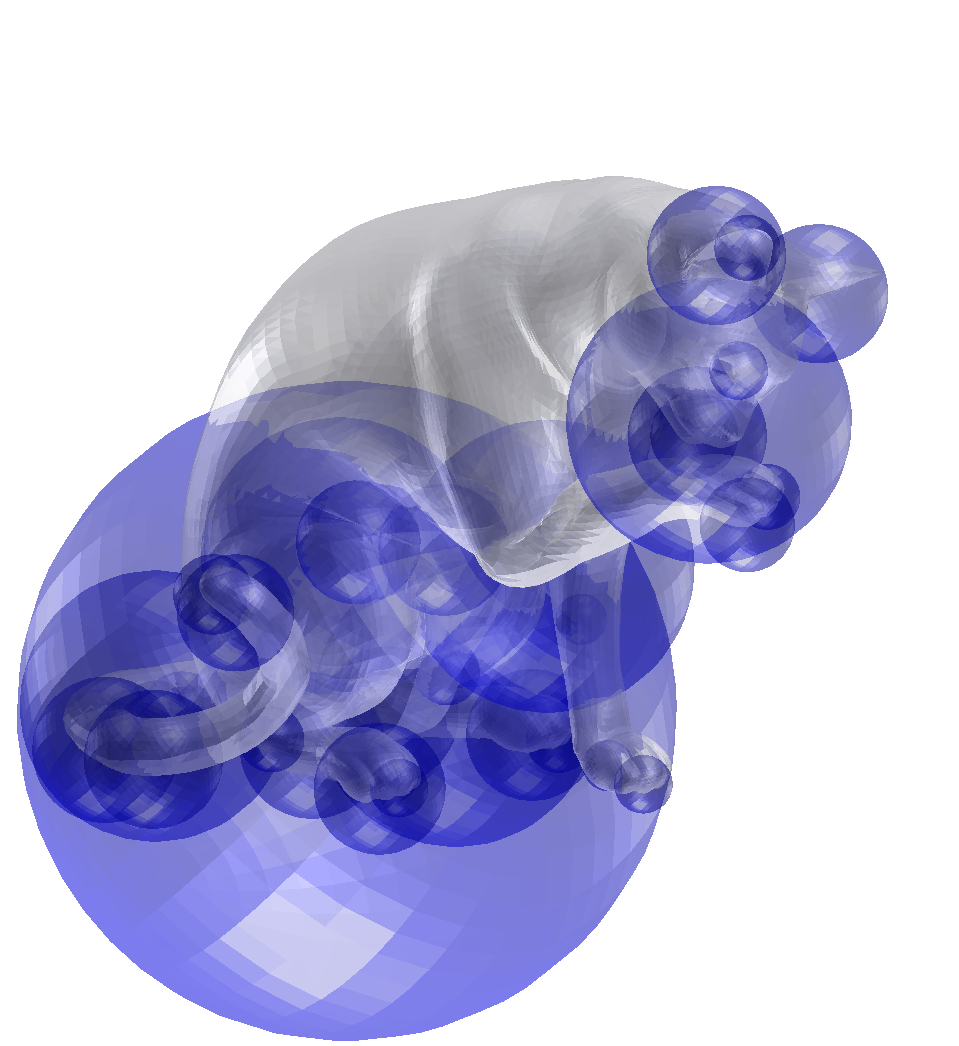
\includegraphics[width=1\linewidth]{./fig/eval/cat_dog.png} 
		\subcaption{DoG}
		\label{fig/eval/testshapes/dog}
	\end{subfigure}
	\begin{subfigure}[t]{0.30\linewidth} 
		\centering 
		\raisebox{-7mm}{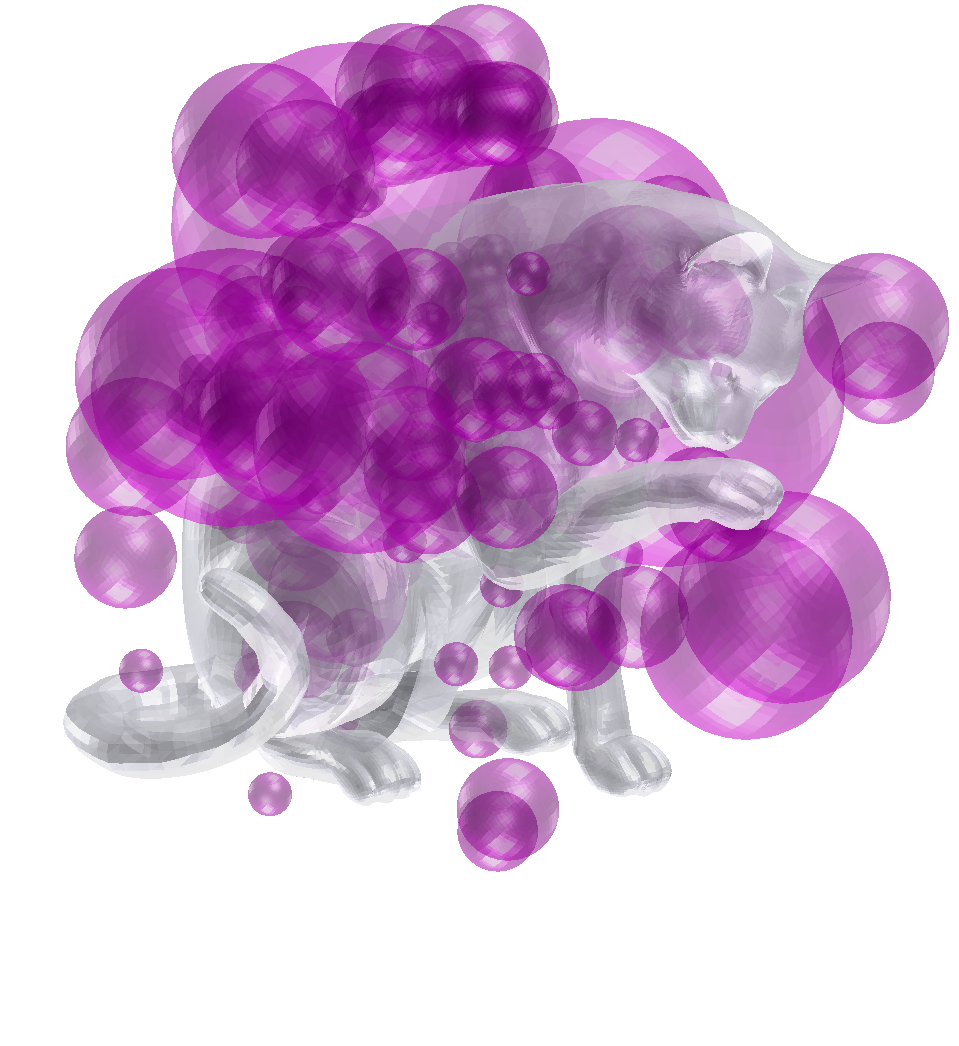
\includegraphics[width=1\linewidth]{./fig/eval/cat_surf.png}}
		\vspace{-7mm}
		\subcaption{SURF}
		\label{fig/eval/testshapes/surf}
	\end{subfigure}
	\begin{subfigure}[t]{0.30\linewidth} 
		\centering 
		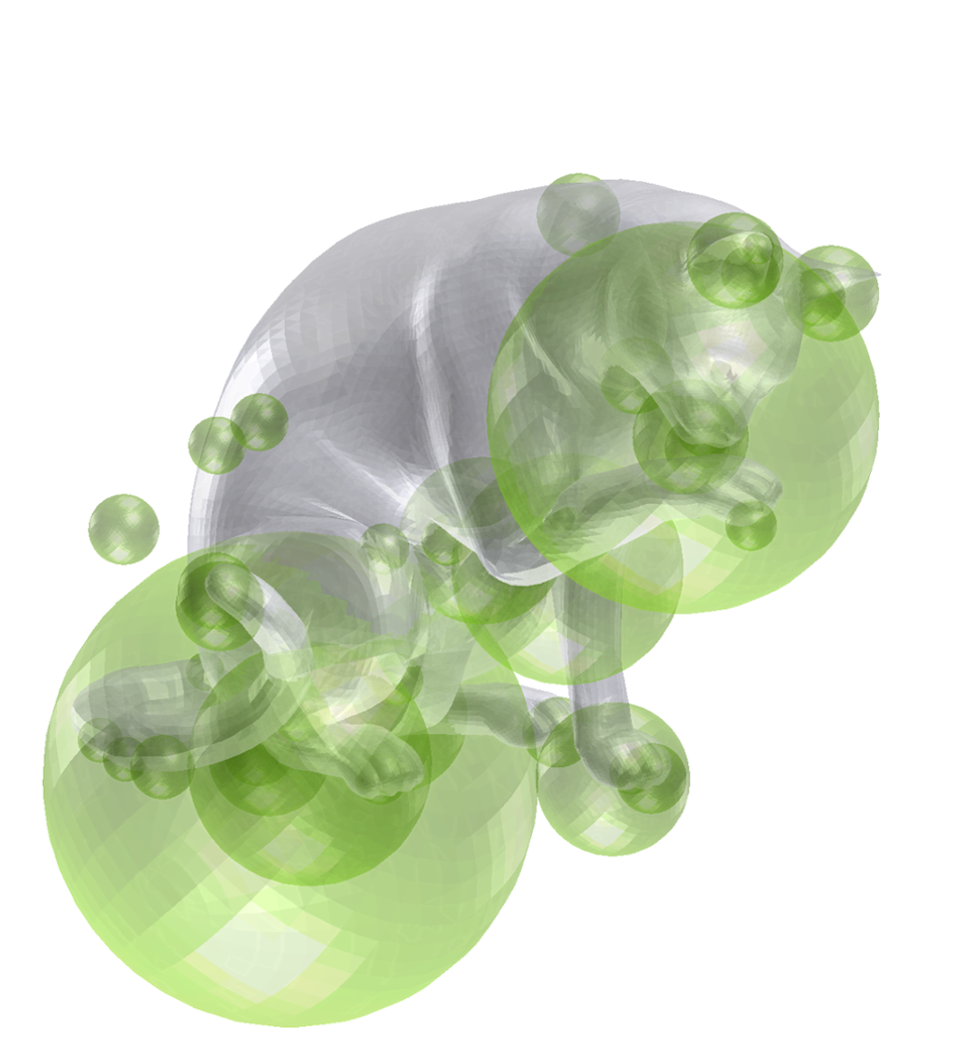
\includegraphics[width=1\linewidth]{./fig/eval/cat_harris.png} 
		\subcaption{Harris}
		\label{fig/eval/testshapes/harris}
	\end{subfigure} \\ 
	\begin{subfigure}[t]{0.30\linewidth} 
		\centering 
		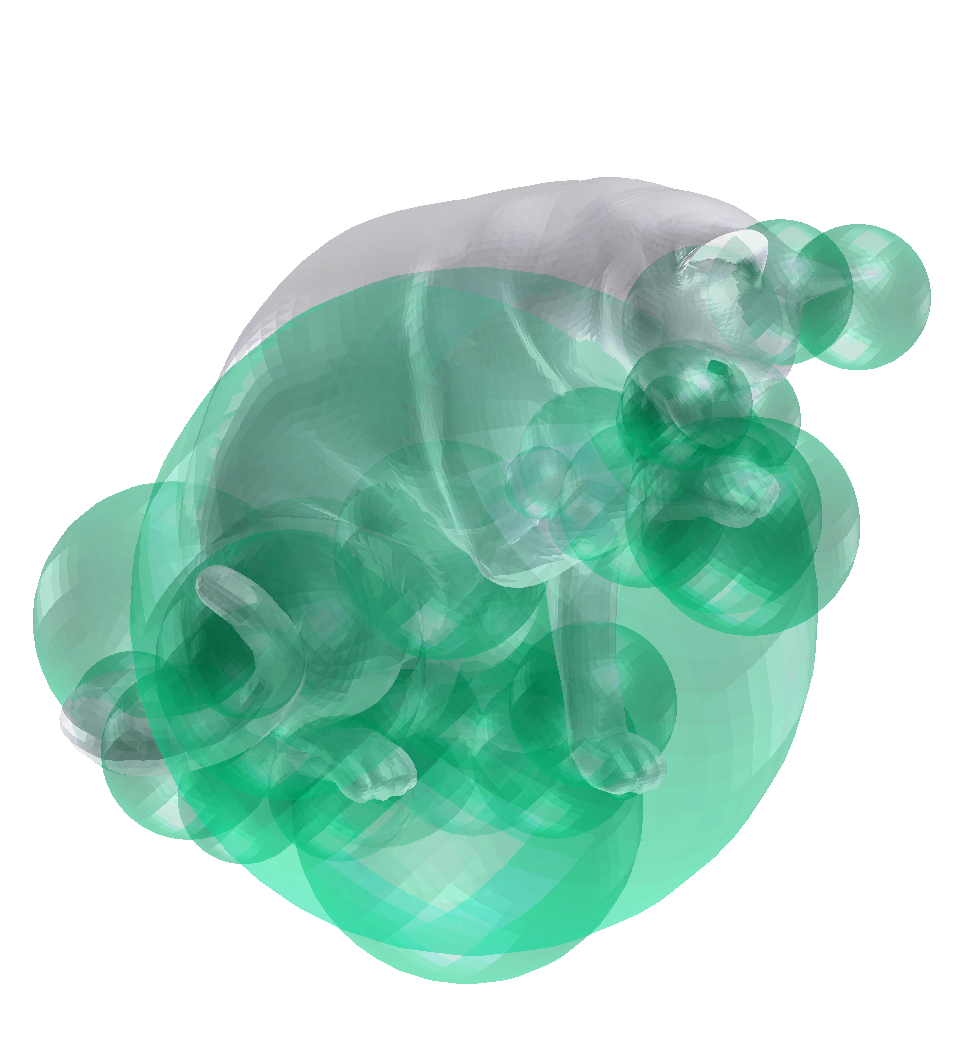
\includegraphics[width=1\linewidth]{./fig/eval/cat_hessian.png} 
		\subcaption{Hessian}
		\label{fig/eval/testshapes/hessian}
	\end{subfigure}
	\begin{subfigure}[t]{0.30\linewidth} 
		\centering 
		\raisebox{-5mm}{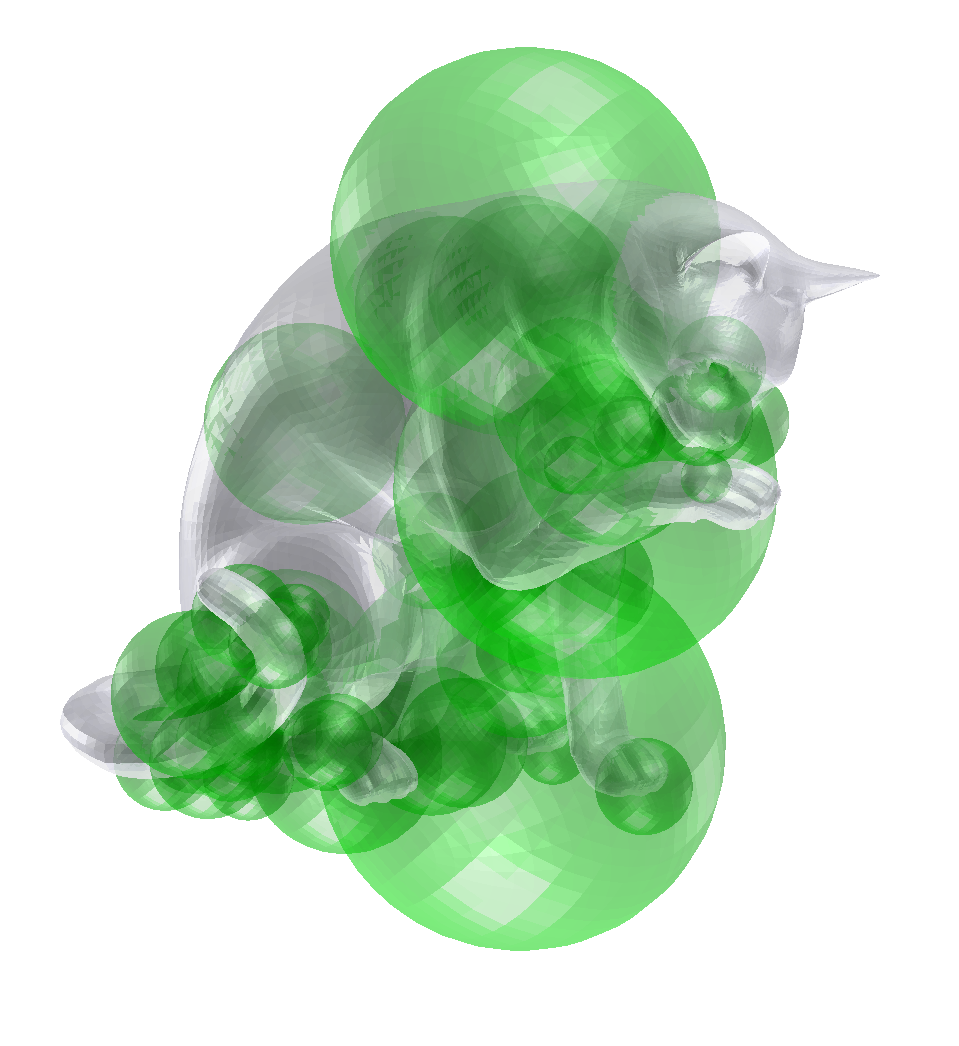
\includegraphics[width=1\linewidth]{./fig/eval/cat_fast.png}}
		\vspace{-5mm} 
		\subcaption{VFAST}
		\label{fig/eval/testshapes/fast}
	\end{subfigure}
	\begin{subfigure}[t]{0.30\linewidth} 
		\centering 
		\raisebox{-3mm}{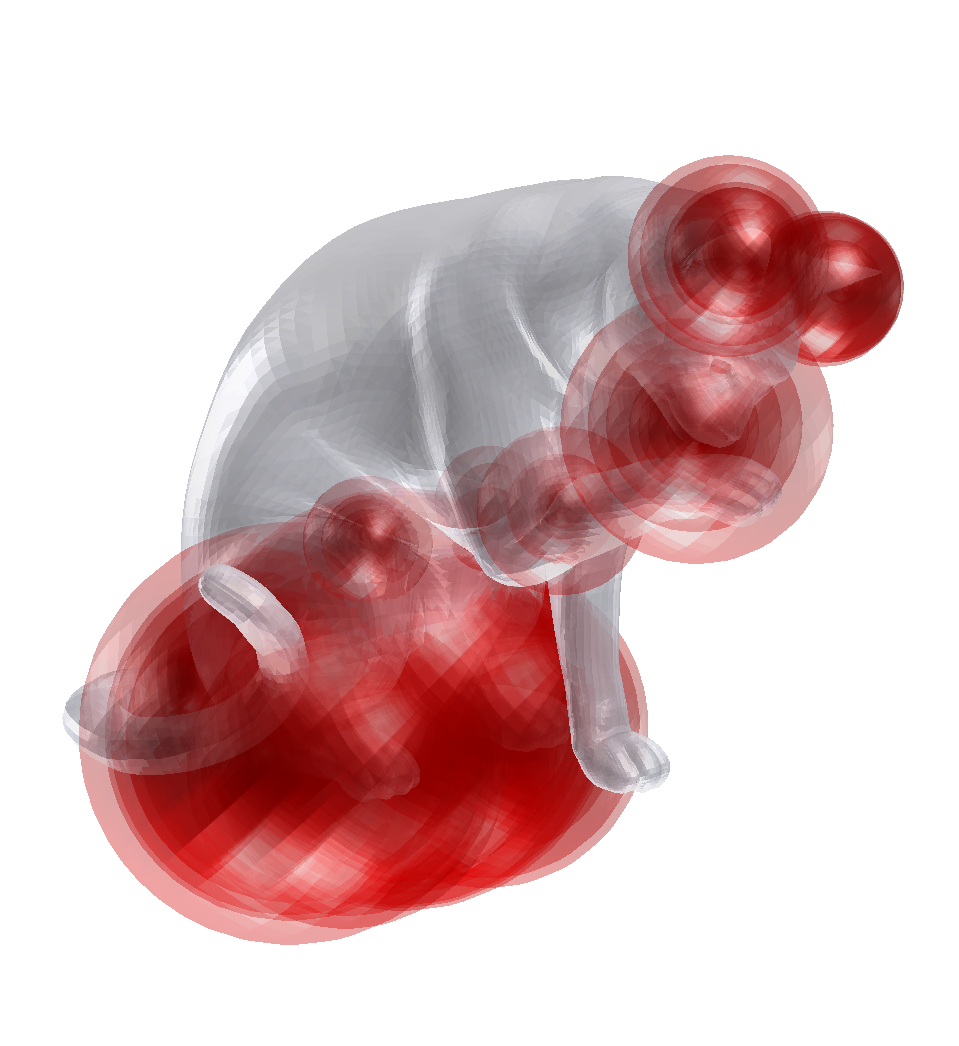
\includegraphics[width=1\linewidth]{./fig/eval/cat_mser.png}}
		\vspace{-5mm}	
		\subcaption{MSER}
		\label{fig/eval/testshapes/mser}
	\end{subfigure}
	\caption{\label{fig/eval/testshapes} \textbf{Volumetric interest points detected on a test 3D shape.}}
\end{figure}

% This paragraph move to introduction! 
\iffalse 
The applications of object detection, recognition and registration are of great importance in computer vision. 
However, advancing geometry capture techniques, in the form of stereo, structured light, structure-from-motion and sensor technologies such as laser scanners, time-of-flight cameras, MRIs and CAT scans, pave the way for the use of shape in these tasks, either on its own or complementing appearance. Whilst an object's appearance is a function not only of its texture, but also its pose and lighting, an object's 3D shape is invariant to all these factors, providing robustness as well as additional discriminative power.
\fi  

% done 
Recognition of 3D data is not a new topic in computer vision \cite{Fisher1987, Nevatia1977, Marr1978, Bolles1983}, though such applications have seen a recent resurgence. Approaches to 3D object recognition range from the local to the global. 

% done 
At the global end are those which form a descriptor from an entire object. Such methods generally offer excellent discrimination plus robustness to shape variation. However, they do not cope well with clutter or occlusion, as they require a complete and segmented object for feature extraction. Also, albeit suitable for recognition, many of the matching algorithms do not consider object pose for registration. 

% done 
At the other end of the spectrum are highly local features, such as points. Being completely non-discriminant, such features are usually embedded in a framework that finds geometrical consistency of features across shapes, \eg iterative closest point (ICP) \cite{Besl1992} and RANSAC \cite{Brown2005, Papazov2011}. 
These geometrical consistency frameworks make matching among 3D instances costly, but they also provide pose for object registration, and the local nature of features provides robustness to clutter and partial occlusion. 

%Between these two extremes are those methods that describe local features of limited but sufficiently distinctive scope, 
However, most existing methods are positioned between the two extremes, where local features describe a limited but sufficiently distinctive scope, thereby leveraging the discriminability of global methods and the robustness of local methods. 
Such features can be used for effective object detection, recognition and registration. The nature of these hybrid methods is reminiscent of the image descriptors of appearance-based methods, not least in the need for shape features to be chosen at points that are repeatably locatable in different datasets, and whose localities are distinctive. 
A common and crucial stage of such approaches is therefore the detection of interest points to be described.  

% done 
This chapter presents a performance evaluation of interest point detectors on scalar volumetric data, as shown in figure \ref{fig/eval/testshapes}.   
As discussed in chapter \ref{chap/intro}, different from other data-specific 3D interest point detectors for meshes \cite{Sipiran2011,Glomb2009,Zaharescu2009} or point-clouds \cite{Aanaes2012,Unnikrishnan2008}, feature detection from scalar volumetric data is versatile. Such data not only comes directly from volumetric sensors, such as MRIs, but can also be generated or converted from other three dimensional data representations, such as point clouds, meshes or depth images, making the proposed evaluation experiments widely applicable to various 3D object recognition systems.
In addition, visual saliency of volumetric interest points is defined in a scalar volume but not on a local surface patch. This full three-dimensional representation implies that interest points can be located off an object's surface, \eg inside a cavity or voxels with varying intensities. 
Furthermore, voxels, which is the 3D equivalent of pixels, make repurposing the many 2D interest point detectors for 3D straightforward. 

% done 
The primary quantitative evaluation criterion used in this work is a novel measure combining both repeatability, based on the number of corresponding points found across two volumes, and the spatial accuracy of correspondences. Detected interest points have a sub-voxel location and a scale, and distances are computed in this space. The qualitative characteristics of the candidate 3D interest point detectors are also presented. 

% no need 
\iffalse 
The following section reviews previous work relevant to interest point detectors and our evaluation framework. Section \ref{sec/eval/detectors} introduces the interest point detectors used in the evaluation experiments, while section \ref{sec/eval/methodology} explains the proposed evaluation methodology.   
Section \ref{sec/eval/experiments} presents the evaluation experiments and their corresponding quantitative and qualitative analyses, before we conclude in section \ref{sec/eval/conclusion}.
\fi 

%-------------------------------------------------------------------------
\section{Related work}
\label{sec/eval/relatedwork}

\subsection{Interest point detectors}

%  done 
The process of interest point detection is the first stage of many object recognition tasks, including object classification and pose estimation. An interest point detector localises salient features from input visual data for further processing. The detected interest points are typically used to match corresponding points across two or more similar sets of data. 
Most early studies focus on detecting features on 2D images. Consequently, the paradigm of 2D interest point detection has already been well studied, for instance Tuytelaars and Mikolajczyk \cite{Tuytelaars2008} performed an extensive survey on locally-invariant feature detectors.  

% done 
Recent advancements in data acquisition techniques have greatly improved the availability of 3D shape data. Large scale synthetic and realistic 3D repositories, such as Google Warehouse \cite{Lai2010} and the B3DO dataset \cite{Janoch2011}, have attracted much interest in shape-based 3D object recognition systems. Consequently, various 3D interest point detection techniques have been proposed alongside with this emerging field of computer vision research. 

% done 
Existing techniques for 3D interest point detection are categorised as volume-based or geometry-based detectors, according to the representation of input data. Volume-based detectors operate directly on the pixel/voxel values of volumetric scalar data. This type of data includes CT scan volumes \cite{Flitton2010}, time-varying video data \cite{Koelstra2009, Laptev2005, Willems2008, Yu2010}, and binary volumes generated from depth images or 3D meshes \cite{Viksten2008, Knopp2010}.  
Geometry-based interest point detectors locate features by extracting geometric information, such as contours, surface normals and surface patches. 
Common data representations of geometry-based techniques include synthetic meshes \cite{Glomb2009,Sipiran2011,Zaharescu2009} or point clouds \cite{Unnikrishnan2008,Aanaes2012}. 
Literature reviews of geometry-based interest point detectors were reported by Salti \etal \cite{Salti2011} and Dutagaci \etal \cite{Dutagaci2011}.  
Nevertheless, unlike 2D interest points, performance evaluation of 3D interest points remains an unexplored topic. 
Hence, this chapter performs the quantitative and qualitative evaluation of volumetric interest point detectors, whose high versatility with respect to original data representation enable a wider coverage of potential applications.

% The remainder of this section will review the interest point detectors used in our evaluation, which we divide into two classes based on their definitions of local features.

% done 
\subsubsection{Corner detection}
The first class of interest point detectors aim to find corners from the input data.
The Harris interest point detector \cite{Harris1988} is a classic image-based corner detection algorithm, which finds points of large gradient changes in orthogonal directions. It detects interest points by analysing the eigenvalues of the second moment matrix (first order derivative). Its 3D adaptations have been applied to registration of volumetric CT scans \cite{Ruiz-Alzola2001, Dalvi2010}.  
Building on the success of Harris corner detector, Mikolajczyk \cite{Mikolajczyk2004} developed the scale-covariant Harris-Laplace detector by finding Harris corners in the spatial domain which are maxima of the Laplacian in the scale domain. 
This approach was extended to space-time interest points for video classification by Laptev \cite{Laptev2005}. 

Instead of detecting corners by image gradients, corner detectors that operate directly on image pixels were also proposed. 
Smith and Brady \cite{Smith1997} presented SUSAN corner detector. It leveraged the proportion of pixels in a neighbourhood, which were dissimilar to the central pixel value.
The FAST corner detector by Rosten \etal \cite{Rosten2010} used the accelerated segment test (AST), a relaxed version of SUSAN, to locate stable corners in an image.  
FAST measures the largest number of contiguous pixels on a circle which are significantly darker, or brighter, than the centre pixel. Without computing the derivative at each pixel, the speed of FAST can also be further improved by learning a decision tree classifier for feature detection. Due to its efficient run-time performance, volumetric feature detectors have been applied to video classification based on FAST interest points \cite{Koelstra2009,Yu2010}. 

\subsubsection{Blob detection}

% done 
Lindeberg \cite{Lindeberg1998} studied scale-covariant interest points using the Laplacian-of-Gaussian kernel, which is mathematically equivalent to the trace of the Hessian, as well as the determinant of the Hessian (DoH). Lowe \cite{Lowe2004} approximated the above LoG kernel by a Difference-of-Gaussians (DoG) operator for better computational performance. Recently, the DoG approach was applied to 3D object detection and recognition of synthetic meshes \cite{Wessel2006}, volumetric scans \cite{Flitton2010} and multi-view stereo data \cite{Pham2011}.

% done 
The Hessian-Laplace detector, by Mikolajczyk and Cordelia \cite{Mikolajczyk2004}, is similar to Harris-Laplace detector. Interest points are detected by evaluating the Hessian matrix of an input image. Similarly, Bay \etal \cite{Bay2008} proposed the speeded-up robust feature (SURF), which accelerated the computation time of determinant-of-Hessian operator using integral images and box filters. Since then SURF has been applied to spatiotemporal data (videos) \cite{Willems2008} and volumetric data generated from synthetic 3D mesh models \cite{Knopp2010}.

% done 
Region-based detector relies on finding salient regions instead of interest points, an example is maximally stable extremal region (MSER) proposed by Matas \etal \cite{Matas2004}. 
While both DoG and SURF are grounded on the approximation of the Laplacian-of-Gaussian kernel, MSER finds thresholded regions whose areas are maximally stable as the threshold changes. 
It is inherently multi-scale, as well as invariant to affine intensity variations and covariant with affine transformations. Three dimensional MSER has already been applied to volumetric data, firstly in the context of segmentation of MRIs \cite{Donoser2006}, and then on video data \cite{Riemenschneider2009}.

\subsubsection{Covariant characteristics}

% done
A feature characteristic is considered covariant when it undergoes the same transformation as the data. 
Image-based detectors have been made affine-covariant, in order to approximate the perspective distortion caused by projection of 3D world onto the 2D image plane \cite{Mikolajczyk2002}. 
Such covariance is not necessary with 3D shapes because most shape acquisition techniques do not have the 3D-2D projection process, thus invariant to view point changes. 
However, objects might have varying poses during data acquisition, such as translation, rotation and scaling for rigid shapes. Rotation and scale covariance are therefore still essential requirements for processing 3D shape data. 
In addition, 3D shape data are generally not affected by illumination and lighting conditions, except for texture-mapped meshes \cite{Zaharescu2009}, the quality of shape data is instead determined by the amount of noise and sampling artefacts, \eg holes and occlusions, from the reconstruction process. 

\subsection{Methodologies}

% done 
Empirical performance evaluation is a popular topic in computer vision, and the evaluation of interest point detectors is no exception. Different approaches of performance evaluations can be categorised according to the evaluation criteria and the source of ground truth interest point locations. 

\subsubsection{Evaluation criteria}

Some methods evaluate performance in the context of a particular task, \eg object recognition \cite{Shin1999, Dutagaci2011}. Such evaluations can be carried out conveniently with a target detector and a ground truth dataset, but they also lack generality to other applications. 

Most evaluation frameworks investigate one or more interest point characteristics. 
One such characteristic, important for registration applications, \eg camera calibration, scene reconstruction and object registration, is the accuracy of interest point localisation. 
Coelho \etal \cite{Coelho1992} measured localisation accuracy by computing projective invariants and comparing these with the actual values measured from the scene. 
Brand and Mohr \cite{Brand1994} introduced three further measures, including 2D Euclidean distance from detected points to ground truth corner locations, given by line fitting to a grid. This approach was extended to using the distance to the nearest point detected in, and transformed from, another image by Schmid \etal \cite{Schmid2000}. 
Laptev \cite{Laptev2003} matched interest points found over location and scale, 
Furthermore, Mikolajczyk \etal \cite{Mikolajczyk2004} used affine transformations to evaluate interest point pairs. 

% done 
For object recognition, two other important characteristics of interest points are their repeatability and distinctiveness. 
Repeatability considers the geometrical stability of the corresponding interest points among multiple input data taken under varying conditions. 
It was proposed and defined by Schmid \etal \cite{Schmid2000} as the ratio of repeated points to detected points. They also introduced entropy, or information content, as a quantitative measure of distinctiveness.
In order to compensate for the effect of the detectors' sensitivity, Rosten \etal \cite{Rosten2010} used the area under the repeatability curve as a function of number of interest points, varied using a threshold on the detector response, in their evaluation. 
When ground truth locations of interest points are given, \eg a pair of hand-labelled images, an alternative measure is the ROC curve, suggested by Bowyer \etal \cite{Bowyer1999}, who considered interest point matching as a binary classification process. Alternatively, qualitative visual comparisons are also used alongside quantitative analyses, on test datasets containing a variety of different interest points \cite{Lindeberg1998, Laptev2005}. Data for qualitative evaluation are often selected to investigate the characteristics of interest points under certain challenging conditions, such as changing camera pose, sampling noise and compression artefacts. 

% done 
In the context of image-based interest points, performance of detectors are often measured over variations in image rotation, scale, viewpoint angle, illumination and noise level \cite{Schmid2000}, as well as corner properties \cite{Rajan1989}. Efficiency is also a further consideration for applications, of which run-time performance is a major concern \cite{Rosten2010}, such as object recognition systems on mobile devices. Nevertheless, evaluations of 3D interest points not only vary on the above-mentioned criteria, but also on the type of data, such as meshes, space-time volumes, point clouds and volumetric scans.

% done 
% It is also worth noting that the distinction between interest point detectors and descriptors. The latter topic, also well evaluated in 2D, \eg \cite{Mikolajczyk2005}, has a concept of both correct and incorrect matches, allowing the use of recall-precision as an evaluation criterion.

% done 
\subsubsection{Ground truth data} 

%With both localisation accuracy and repeatability criteria, the ground truth location of interest points in the scene must be known. The ground truth data can be computed in a variety of ways. 
In order to compute any of the aforementioned interest point characteristics, the ground truth locations of interest points, or the ground truth homography between two evaluation instances, must be known. Ground truth information can be obtained in a variety of ways.  
Several approaches specify the location of interest points in an image, either known by design \cite{Rajan1989}, or hand-labelled by multiple people \cite{Heath1997}. 
Other methods find corresponding pairs of point across two or more images. For example, matching is achieved using planar scenes and computing homographies between images \cite{Schmid2000}, scenes of known geometry manually registered in each image \cite{Rosten2010}, scene geometry captured using structured light \cite{Aanaes2012} and synthetic data \cite{Laptev2005}. 
In addition, ground truth data for 3D interest point evaluations are likewise obtained from manual annotation \cite{Dutagaci2011}, known projection homography of stereo point clouds \cite{Aanaes2012} and synthetic shape data \cite{Salti2011}. 

% done 
\section{Detectors}
\label{sec/eval/detectors}

Generally every new volumetric interest point was proposed with an application in mind, such as shape retrieval and classification \cite{Riemenschneider2009,Flitton2010,Knopp2010,Prasad2011}, medical imaging \cite{Criminisi2011,Ni2008,Donner2011} and video classification \cite{Willems2009,Laptev2005,Yu2010}. 
Whilst interest point detectors for images have already been studied extensively \cite{Mikolajczyk2005, Tuytelaars2008}, evaluation of 3D interest points is still an unexplored area. 

This section describes the principles and formulations of the 3D interest points evaluated in the experiments. These include DoG \cite{Flitton2010, Pham2011}, DoH and Harris-based interest points \cite{Laptev2005}, SURF \cite{Willems2008, Knopp2010}, VFAST \cite{Yu2010} and MSER \cite{Donoser2006, Riemenschneider2009}. 

\subsection{Scale-space and sub-voxel refinement}
\label{sec/eval/subvoxel}

% done 
Scale covariance of interest points is achieved by creating a scale-space of the input volumetric data. An octave of linear scale-space is created by convolving the input volume with a Gaussian smoothing kernel. Such smoothing kernel is applied on the volume recursively to suppress fine-scale structures. Afterwards a new octave is created by down-sampling the input volumes from the previous octave. As a result, a series of volumes, with multiple levels of details, is created. The implementation of scale-space, with respect to interest point detection, has been detailed by Lindeberg \cite{Lindeberg1998}. 

% done 
However, scale-space representation is not computed for MSER because it detects salient regions in different scales. MSER locates interest points by fitting an ellipsoid to the detected salient region \cite{Matas2004}. For other interest point detectors, saliency responses are computed in all volumes within the scale-space. In addition, the subpixel refinement process in SIFT \cite{Lowe2004} is applied on these detectors. Interest points are localised at the sub-voxel level by fitting 4D quadratic functions around the local scale-space maxima, and selecting the maxima of those functions instead. 

% done 
\subsection{Difference-of-Gaussians (DoG)}
The DoG operator is a blob detection technique for feature localisation popularised by the SIFT algorithm \cite{Lowe2004}. DoG approximates the Laplacian-of-Gaussian filter, which detects features of a particular size. 
The saliency response of DoG detector $S_{\textrm{DoG}}$ is computed by subtracting two Gaussian smoothed volumes, usually adjacent scale-space representations, of the same input data and taking the absolute values of the difference.
Interest points are detected at the 4D local maxima, \ie 3D space plus scale, with respect to the saliency response $S_{\textrm{DoG}}$ within each octave of $\mathbf{v}(\mathbf{x},\sigma_s)$: 
\begin{equation}
	\label{eqn/eval/dog} 
	% S_{\textrm{DoG}}(x,y,z;\sigma_s) = \bigg|V(x,y,z;\sigma_s) - V(x,y,z;\sigma_{s-1})\bigg|.
	S_{\textrm{DoG}}(\mathbf{x};\sigma_s) = \bigg|\mathbf{v}(\mathbf{x};\sigma_s) - \mathbf{v}(\mathbf{x};\sigma_{s-1})\bigg|.
\end{equation}
Volume $V(x,y,z;\sigma_s)$ denotes the scale-space representation of the input volumetric data at scale $\sigma_s$.

\subsection{Harris}
Harris corner detector examines image gradients by shifting in a local window, interest points are detected at positions where large changes are observed in all directions \cite{Harris1988}. While the first 3D extension of the original Harris corner detector uses separate scale parameters for the heterogeneous space and time axes \cite{Laptev2005}, in this work only one scale $\sigma_s$ is shared among three homogeneous spatial axes for simplicity.  
The second-moment matrix $\mathbf{M}$ is computed by smoothing the first derivatives of the volume in scale-space $\mathbf{v}(\mathbf{x};\sigma_s)$ by a spherical Gaussian kernel $g(\cdot;\sigma_\textrm{Harris})$: 
\begin{equation}
	\begin{aligned}
		\mathbf{v}_x(\mathbf{x};\sigma^2_s) & = \displaystyle\frac{\partial \mathbf{v}(\mathbf{x};\sigma^2_s)}{\partial x}, \\
		\mathbf{v}_y(\mathbf{x};\sigma^2_s) & = \displaystyle\frac{\partial \mathbf{v}(\mathbf{x};\sigma^2_s)}{\partial y}, \\
		\mathbf{v}_z(\mathbf{x};\sigma^2_s) & = \displaystyle\frac{\partial \mathbf{v}(\mathbf{x};\sigma^2_s)}{\partial z}, \\ 
		\mathbf{M}(\cdot, \sigma_\textrm{Harris}, \sigma_s) & = g(\cdot;\sigma_\textrm{Harris}) \ast \left[
			\begin{array}{ccc}
				\mathbf{v}^2_x & \mathbf{v}_x\mathbf{v}_y & \mathbf{v}_x\mathbf{v}_z \\
				\mathbf{v}_x\mathbf{v}_y & \mathbf{v}_y^2 & \mathbf{v}_y\mathbf{v}_z \\
				\mathbf{v}_x\mathbf{v}_z & \mathbf{v}_y\mathbf{v}_z & \mathbf{v}^2_z \\
			\end{array}
		\right],
	\end{aligned}
	\label{eqn/eval/harris_2ndmoment}
\end{equation}
where $\mathbf{v}_x$,$\mathbf{v}_y$,$\mathbf{v}_z$ denote the partial derivatives of the volume in scale-space $\mathbf{v}(\mathbf{x};\sigma_s)$ along $x$, $y$ and $z$ axes respectively. The second moment matrix $\mathbf{M}$ describes the auto-correlation along different directions in a local neighbourhood of size $\sigma_s$. 

Candidate interest points are located at coordinates $(x,y,z)$ where the second-moment matrix $\mathbf{M}(x,y,z; \sigma_\textrm{Harris}, \sigma_s)$ has large eigenvalues. Interest point are selected at the 4D local maxima in the scale-space of $S_{\textrm{Harris}}$. Locations of interest points are refined using the sub-voxel refinement method described in section \ref{sec/eval/subvoxel}. The window size $\sigma_\textrm{Harris}$ is proportional to expected feature scales $\sigma_s$ by a factor of $0.7$ as suggested by Mikolajczyk and Cordelia \cite{Mikolajczyk2004}. 

The saliency response of Harris corner, $S_\textrm{Harris}$, is computed from the determinant and trace of the second-moment matrix $\mathbf{M}$: 
\begin{equation}
	S_\textrm{Harris} = \sigma_{s}^3 \:\det(\mathbf{M}) - \kappa\:\mathrm{Tr(\mathbf{M})}^3,
	\label{eqn/eval/harriscorner}
\end{equation}
where $\kappa$ is a tunable sensitivity parameter that controls the reject of edge points.  
Saliency response $S_\textrm{Harris}$ is normalised by its scale $\sigma_s$ in equation \ref{eqn/eval/harriscorner}.

% done 
\subsection{Determinant-of-Hessian (DoH)}
\label{sec/eval/doh}
The DoH interest point is similar to the Harris detector with respect to formulation \cite{Lindeberg1998}. Instead of second-moment matrix, a Hessian matrix $\mathbf{H}$ is computed from $\mathbf{v}$: 
\begin{equation}
	\mathbf{H} = 
	\left[
		\begin{array}{ccc}
			\mathbf{v}_{xx} & \mathbf{v}_{xy} & \mathbf{v}_{xz} \\
			\mathbf{v}_{yx} & \mathbf{v}_{yy} & \mathbf{v}_{yz} \\
			\mathbf{v}_{zx} & \mathbf{v}_{zy} & \mathbf{v}_{zz} 
		\end{array}
	\right],
	\label{eqn/eval/hessianmatrix}
\end{equation}
where $\mathbf{v}_{xy}$ denotes the second derivative of the volume at scale $\sigma_s$, along $x$ and $y$ axes, such that
\begin{equation}
	\mathbf{v}_{xy} = \displaystyle\frac{\partial \mathbf{v}(\mathbf{x};\sigma_s)}{\partial x \partial y}.
	\label{eqn/eval/hessiandiverative}
\end{equation}
The saliency response is the scale-normalised determinant of Hessian matrix $\mathbf{H}$:
\begin{equation}
	S_{\textrm{Hessian}} = \sigma^3_s \:\mathrm{det}(\mathbf{H}).
	\label{eqn/eval/hessiansaliency}
\end{equation}
Subsequently, interest points are located at the 4D scale-space local maxima of $S_\textrm{Hessian}$.

% done 
\subsection{SURF}
Speeded up robust features (SURF) is a feature extraction algorithm optimised for efficiency \cite{Bay2008}. The 3D, volumetric version of SURF was first introduced by Willems \etal \cite{Willems2008} for video classification. Recently, it was used in a 3D shape object recognition task \cite{Knopp2010}.

SURF is an efficient approximation of the DoH detector. Second-order derivatives of Gaussians in the DoH detector are approximated by six Haar wavelets, \ie box filters. Convolutions of the Haar wavelets can be greatly accelerated using integral videos/volumes. The saliency response of 3D SURF is similar to the aforementioned DoH detector. 

% done 
\subsection{VFAST}
\label{sec/eval/vfast}

Building on the success of the FAST corner detector \cite{Rosten2010}, VFAST \cite{Yu2010} and FAST-3D \cite{Koelstra2009} have been introduced to video-based object classification. 
The VFAST interest points are detected by directly comparing intensities in the video sequences. Similar to FAST, the VFAST detector can be further accelerated by learning a decision tree-based corner detector from training videos \cite{Rosten2010}. 

The VFAST algorithm performs accelerated segment tests (AST) on three orthogonal planes, $XY$, $XZ$ and $YZ$. The saliency score is computed by maximising the differences $\{ t_{XY}, t_{XZ}, t_{YZ} \}$ that makes at least $n$ contiguous voxels brighter or darker than the nucleus voxel $\vxpatch(x,y,z)$ by a threshold $\delta_{V}$. Consider the voxels values $\becire_{XY}$ on the $XY$ Bresenham circle $\becir_{XY}$, $AST(x,y,z)$ is computed:  
\begin{align}
	t_{XY} & = \max\left(| \vxpatch(x,y,z) > \becire_{XY}|,\;\forall \becire_{XY} \in \becir_{XY} \right)\\ 
AST_{XY}(x,y,z) & = \left\{
\begin{array}{lr}
	t_{XY} & \mbox{if $> n$ contiguous } |\vxpatch(x,y,z) - \becire_{XY}| > \delta_{V} \\
	0 & \mbox{ otherwise }
\end{array}
\right..
\label{eqn/eval/fastast}
\end{align}
Subsequently, the combined saliency response $S_{\textrm{vfast}}$ is the Euclidean norm of saliency scores on the three planes: 
\begin{equation}
S_\textrm{vfast} = \sqrt{ \left(AST_{XY}(x,y,t)\right)^2+ \left(AST_{XZ}(x,y,t)\right)^2+ \left(AST_{YZ}(x,y,t)\right)^2}.
\label{eqn/eval/fastverall}
\end{equation}
Interest points are detected at the local maxima in $S_{\textrm{vfast}}$ over both translation and scale, with at least two non-zero responses in $AST_{XY}(n,t)$, $AST_{XZ}(n,t)$ and $AST_{YZ}(n,t)$. The steps of computing VFAST interest points are described in algorithm \ref{algo/eval/vfast}. 

\begin{algorithm}
\caption{\textbf{VFAST interest point detector}}
\label{algo/eval/vfast}
\begin{algorithmic}
	\REQUIRE $[x,y,z] = $ voxel coordinates
	\REQUIRE $r_{XY},r_{XZ},r_{YZ} = $ radii of Bresenham circles
	\REQUIRE $n = $ contiguous threshold
	\REQUIRE $\delta_{V} = $ intensity threshold
	\STATE $\becir_{XY},\becir_{XT},\becir_{YT}$ = Pixels of Bresenham circles
	\STATE $t_{XY} = \max\left(| \vxpatch(x,y,z) > \becire_{XY}|; \forall \becire_{XY} \in \becir_{XY} \right)$
	\STATE Compute $AST_{XY}(x,y,z)$ by equation \ref{eqn/eval/fastast}
	\STATE Compute $AST_{XZ}(x,y,z)$ accordingly 
	\STATE Compute $AST_{YZ}(x,y,z)$ accordingly 
	\STATE Compute $S_\textrm{vfast}$ by equation \ref{eqn/eval/fastverall}
	\STATE Discard pixels that has only one non-zero $AST(\cdot)$ function 
	\STATE Detect interest points at the 4D local maxima 
\end{algorithmic}
\end{algorithm}

% done 
\subsection{MSER}
The maximally stable extremal regions (MSER) detector is a region-based blob detection technique proposed by Matas \etal \cite{Matas2004}. Extremal regions are the connected components of a thresholded input data, which can be an image or a volume. Maximally stable regions are selected from a set of nested extremal regions obtained using different thresholds. The extremal regions of an input volume can be enumerated efficiently using the union-find algorithm which has a worst case of $O(N\log(\log(N)))$ \cite{Matas2004}, where $N$ is the number of pixels/voxels. 
Being essentially robust to rotation and scale changes, MSER has been applied to detection of volumetric regions \cite{Donoser2006,Riemenschneider2009}.

Normally an ellipsoid is fitted to each maximally stable region from the input data \cite{Matas2004}, the position and scale of MSER interest points being represented by the centres and radii of such ellipsoids respectively. In this work a sphere is fitted to the stable regions instead, making the interest points compatible with the proposed evaluation framework.

% done 
\section{Methodology}
\label{sec/eval/methodology}

The traditional repeatability ratio measures the repeatability of interest point detectors at a single, predefined accuracy \cite{Schmid2000}; it is not only sensitive to the choice of matching distance threshold, but also gives little indication of the actual localisation accuracy, \ie the closeness of corresponding interest points, for correspondences, other than that they fall within the threshold. Hence, a single repeatability ratio is insufficient to describe the performance of interest point detectors for various applications with different accuracy requirements. 

On the other hand, real matching accuracy, \eg ROC curves \cite{Bowyer1999}, requires hand crafted point-to-point ground truth correspondences. This approach is difficult to generalise to large, realistic evaluation datasets such as point clouds from multi-view stereo systems.     

Whilst existing evaluations focused on either localisation accuracy or repeatability, a new performance is used in this work, by combining the two qualities. The proposed combined score is computed based on \emph{repeatability ratio} with respect to \emph{varying accuracy} requirements. This section explains the combined score used in the experiments. 

% done 
\subsection{Localisation accuracy}
An interest point is considered as a sphere at coordinates $\{\pointx, \pointy, \pointz\}$ in a voxelised 3D space, with radius $\pointscale$ given by its scale. A vector $\onepoint$ is used to describe this interest point by concatenating its spatial location and scale: 
\begin{equation}
	\onepoint = \big[ \pointx,\;\pointy,\;\pointz,\;\scalefactor\log(\pointscale) \big]^\mathsf{T}.
\label{eqn/eval/loc_vec}
\end{equation}
The logarithm of scale is used to remove multiplicative bias across detectors, and since spatial location and scale are not fully commensurate, a tunable parameter $\scalefactor$ is introduced to weight the importance of scale to the distance function.

A key component of the proposed evaluation score is the distance metric for measuring the closeness of two corresponding interest points with respect to their locations and scales. In this work, the Euclidean norm is used:
\begin{equation}
	D(\onepoint, \anotherpoint') = \big|\big|\onepoint - \anotherpoint'\big|\big|_{2},
	\label{eqn/eval/matchdistance}
\end{equation}
% A key component of the proposed evaluation score is the distance metric for measuring the closeness of two corresponding interest points with respect to their locations and scales. 
%An interest point $\onepoint$ is represented by a sphere at coordinates $[\pointx, \pointy, \pointz]$ with radius $\pointscale$ given by scale.   
%\begin{equation}
%D(\onepoint, \anotherpoint') = ||\onepoint - \anotherpoint'||_2
%\label{eqn/eval/matchdistance}
%\end{equation}
%A key component of the proposed evaluation score is the distance metric used to measure the closeness of two corresponding interest points with respect to their locations and scales:
%\begin{equation}
%\onepoint = [\pointx,~\pointy,~\pointz,~f\log \pointscale]^\mathrm{T}
%\label{eqn/eval/loc_vec}
%\end{equation}
%The log of scale is used to remove multiplicative bias across detectors, and since spatial location and scale are not fully commensurable, a parameter $f$ is introduced to balance the importance of scale to the distance function. 
where $\onepoint$ is the coordinate of an interest point found in the volume, $\volumep$, and $\anotherpoint'$ is the point $\anotherpoint$ found in another volume $\volumeq$, transformed into the coordinate frame of $\volumep$ using a known ground truth homography. The evaluation score is the distance of an interest point to the nearest transformed interest point:
\begin{equation}
D(\onepoint, \anotherpointset') = \min_{\anotherpoint'_j \in \anotherpointset'}D(\onepoint, \anotherpoint'_j),
\label{eqn/eval/metricNN}
\end{equation}
where $\anotherpointset'$ denotes the set of all $q$ transformed interest points $\{\anotherpoint'_j\}_{j=1}^{q}$ detected in $\volumeq$.

% done
\subsection{Repeatability}
Schmid \etal \cite{Schmid2000} defined repeatability as the ratio of correspondences to points:
\begin{equation}
R_\textrm{ratio}(\onepointset, \anotherpointset', \disp) = \frac{\displaystyle\sum_{i=1}^p H\left(D(\onepoint_i, \anotherpointset') - \disp\right)}{\min(p, q)},
\label{eqn/eval/repeatratio}
\end{equation}
where $\onepointset = \{\onepoint_i\}_{i=1}^{p}$, the set of $p$ interest points found in $\volumep$, and $\disp$ is a user provided distance threshold. 
The Heaviside step function $H(\cdot)$ returns $1$ when the input is positive, $0$ otherwise.
This repeatability measure favours dense interest points over accurate but sparse interest points \cite{Willis2009}. 
However, it does not affect the fairness of this evaluation framework because fully-overlapped object pairs are used.
%In addition, the symmetry of the combined $\areascore$ score \ref{eqn/eval/rptarea} cancels out the effect of differences in interest points' density.

% done
\subsection{Combined score}
Rosten \etal \cite{Rosten2010} computed the area under $R_\textrm{ratio}$ as a function of the number of interest points. 
The same principle is applied in the proposed evaluation metric, but it is computed using the repeatability ratio $R_\textrm{ratio}$ under varying distance threshold, $\disp$.  
The proposed score therefore increases both if a higher proportion of points are matched, and also if matches are more accurate. 

Such combined score is not symmetric with respect to testing instances $\volumep$ and $\volumeq$, symmetry of evaluation score is enforced by computing the average score across two matching directions, using $\volumep$ and $\volumeq$ as the reference frames respectively, in order to compensate for the effect of different interest point densities among the testing instances. Finally, the evaluation score is given as the area under the $\disp$ \textit{versus} $R_\textrm{ratio}$ curve within a maximum matching distance $D$, such that  
\begin{equation}
\areascore=\frac{1}{2D}\int_{0}^{D}R_\textrm{ratio}(\onepointset, \anotherpointset', \disp) + R_\textrm{ratio}(\anotherpointset, \onepointset', \disp) ~ \textrm{d}\disp.
\label{eqn/eval/rptarea}
\end{equation}
The $\areascore$ score is advantageous over the original repeatability ratio, as it reflects both repeatability and accuracy of interest points in one measurement. 

% done 
\section{Experiments}
\label{sec/eval/experiments}

This section describes a comprehensive evaluation of the candidate 3D interest point detectors, investigating their performances under different variations of input data, \eg rotation or sampling noise. Quantitative evaluations were performed by computing the proposed combined repeatability scores $\areascore$ for each candidate detector, using a synthetic dataset with pre-computed ground truth homographies. Interest point detectors were then analysed qualitatively using real-life shape data, namely MRIs and multi-view stereo data. 

\subsection{Datasets}
\label{sec/eval/testdata}

\begin{figure}[ht]
	\centering
	\begin{subfigure}[t]{0.31\linewidth} \centering 
		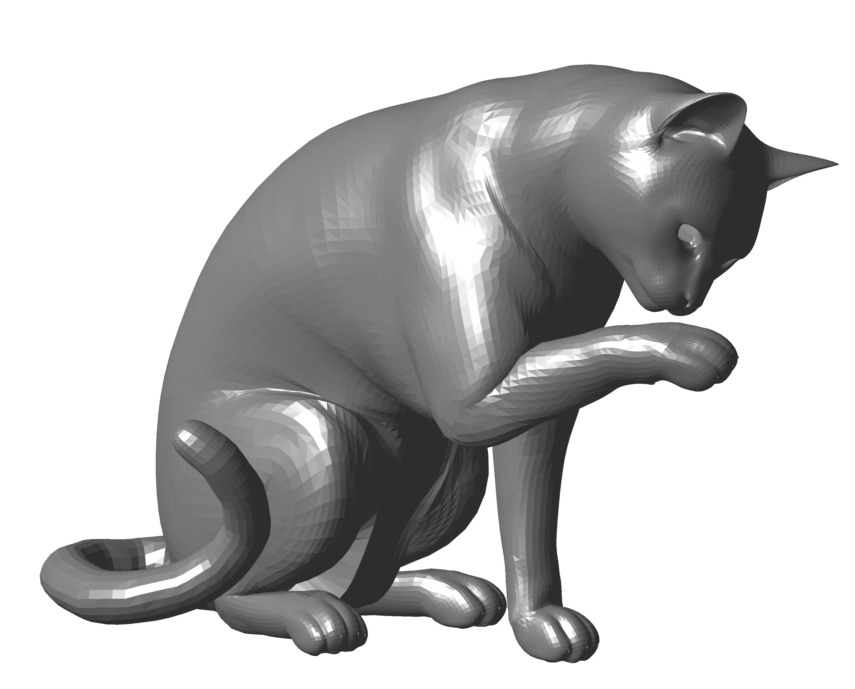
\includegraphics[height=0.85\linewidth]{./fig/eval/cat_mesh.png} 
		\subcaption{Mesh} 
	\end{subfigure}
	\begin{subfigure}[t]{0.31\linewidth} \centering
		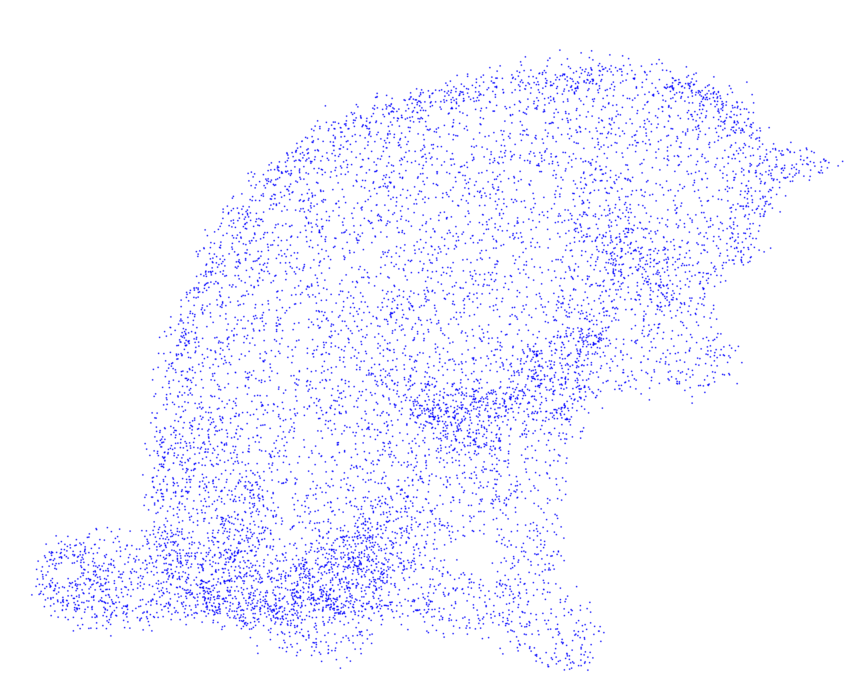
\includegraphics[height=0.85\linewidth]{./fig/eval/cat_points.png}
		\subcaption{Point cloud} 
	\end{subfigure}
	\begin{subfigure}[t]{0.31\linewidth} \centering 
		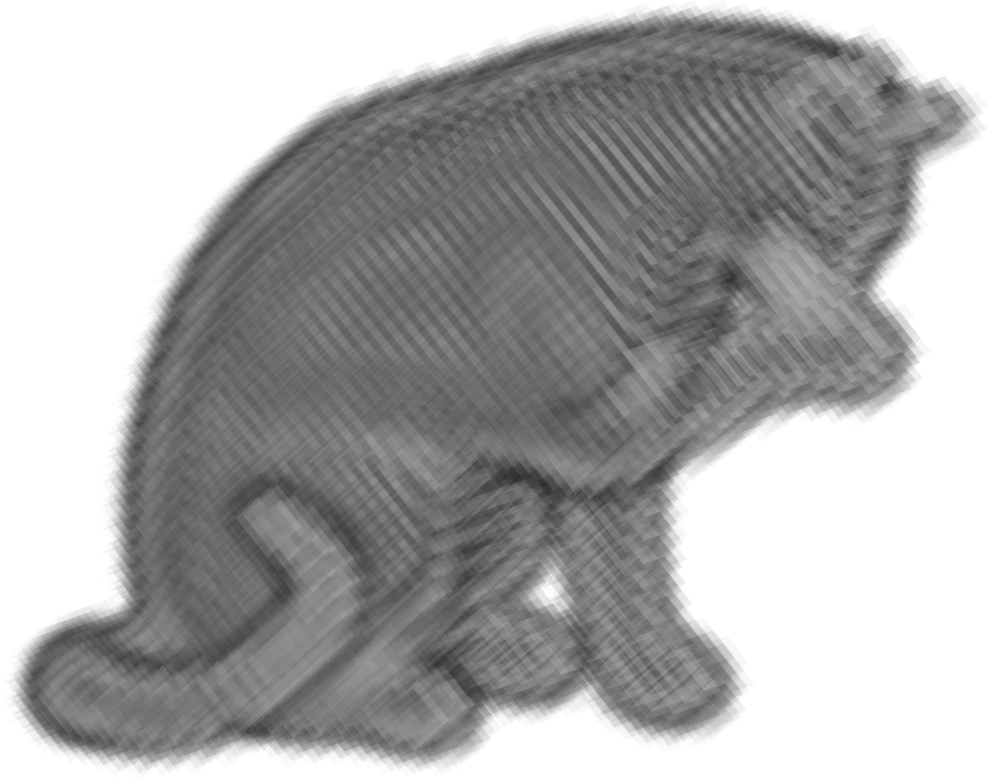
\includegraphics[height=0.85\linewidth]{./fig/eval/cat_volume.png}
		\subcaption{Voxel array} 
	\end{subfigure}
	\caption{\textbf{Mesh to volume conversion.} Left to right: mesh, point cloud and voxel array.} 
	\label{fig/eval/vol_conversion}
\end{figure}

% done 
Three different datasets were used in the evaluation experiments. Two of them are synthetic, as large sets of real, registered, 3D data with known ground truths were not commonly available. Synthetic data were used because new test data can be generated and modified easily, \eg controllable noise levels, transformations and sampling densities. Accurate ground truths were generated with the synthetic test data for evaluation.  
From the graphs in figure \ref{fig/eval/graph2}, synthetic and real testing data produce comparable results in the evaluation experiments. 

% done 
The first set, the \meshset dataset, contains $25$ shapes (surface meshes) chosen from the Princeton Shape Benchmark \cite{Shilane2004} and the TOSCA \cite{Bronstein2008} dataset. 
This dataset includes a wide range of geometric features, ranging from coarse structures to fine details, as illustrated in figure \ref{fig/eval/sampleshapes}. In the experiment, point clouds were created by sampling 3D points, with a uniform distribution, over the surfaces of the meshes. Gaussian white noise was added to the points to simulate measurement errors introduced during 3D shape acquisition. 
The point clouds were subsequently voxelised using kernel density estimation with a Gaussian kernel $g(\cdot,\sigma_{KDE})$ as shown in figure \ref{fig/eval/vol_conversion}.
%This conversion process allows sampling density and noise to be varied when generating the volumes.
Finally, a linear scale-space $\mathbf{v}(\mathbf{x};\sigma_s)$ was created from each volume, in order to detect shape features at different scales, \cf \ref{sec/eval/subvoxel}. All shapes in the dataset underwent this conversion process. 

% done 
The \mriset dataset consists of two synthetic MRI scans of a human brain, generated from BrainWeb simulated brain database \cite{Cocosco1997}. The ground truth homographies ($20^{\circ}$ rotation and $20$ voxel translation) between the two MRI scans are given for performance evaluation. Since MRI scans are inherently volumetric, voxelisation is not necessary. 

% done 
The third \stereoset dataset contains a series of $16$ point clouds of $8$ objects from the Toshiba CAD model point clouds dataset \cite{Pham2011}, which were captured using a photometric, multi-view stereo system \cite{Vogiatzis2011}. Relative transformations were computed by aligning each point cloud with a reference model using the ICP algorithm \cite{Besl1992} and then refining the registration manually. The same voxelisation technique was used to convert stereo point clouds to volumetric data.

% done 
In the \meshset and the \stereoset datasets, high-intensity voxels are located at the object surface, leaving the interior of the shapes hollow as low-intensity voxels. In contrast, the interior of the \mriset data is filled with voxels of different intensities. The experimental results in the next section have demonstrated different behaviours of the detectors in these two voxelisation scenarios.

% done 
While the synthetic shape instances of the same object completely overlap one another, avoiding bias to the repeatability score mentioned in Willis and Sui \cite{Willis2009}, the real stereo data contain occlusions. While the underside of each object, which varied across instances, was not captured, the shapes in \stereoset were captured with uneven sampling density and generally more sampling noise. The feasibility of performance evaluation using synthetic data is therefore verified by comparing the results on the \meshset dataset with those on the \stereoset dataset. 

%\begin{figure}[ht]
%\centering
%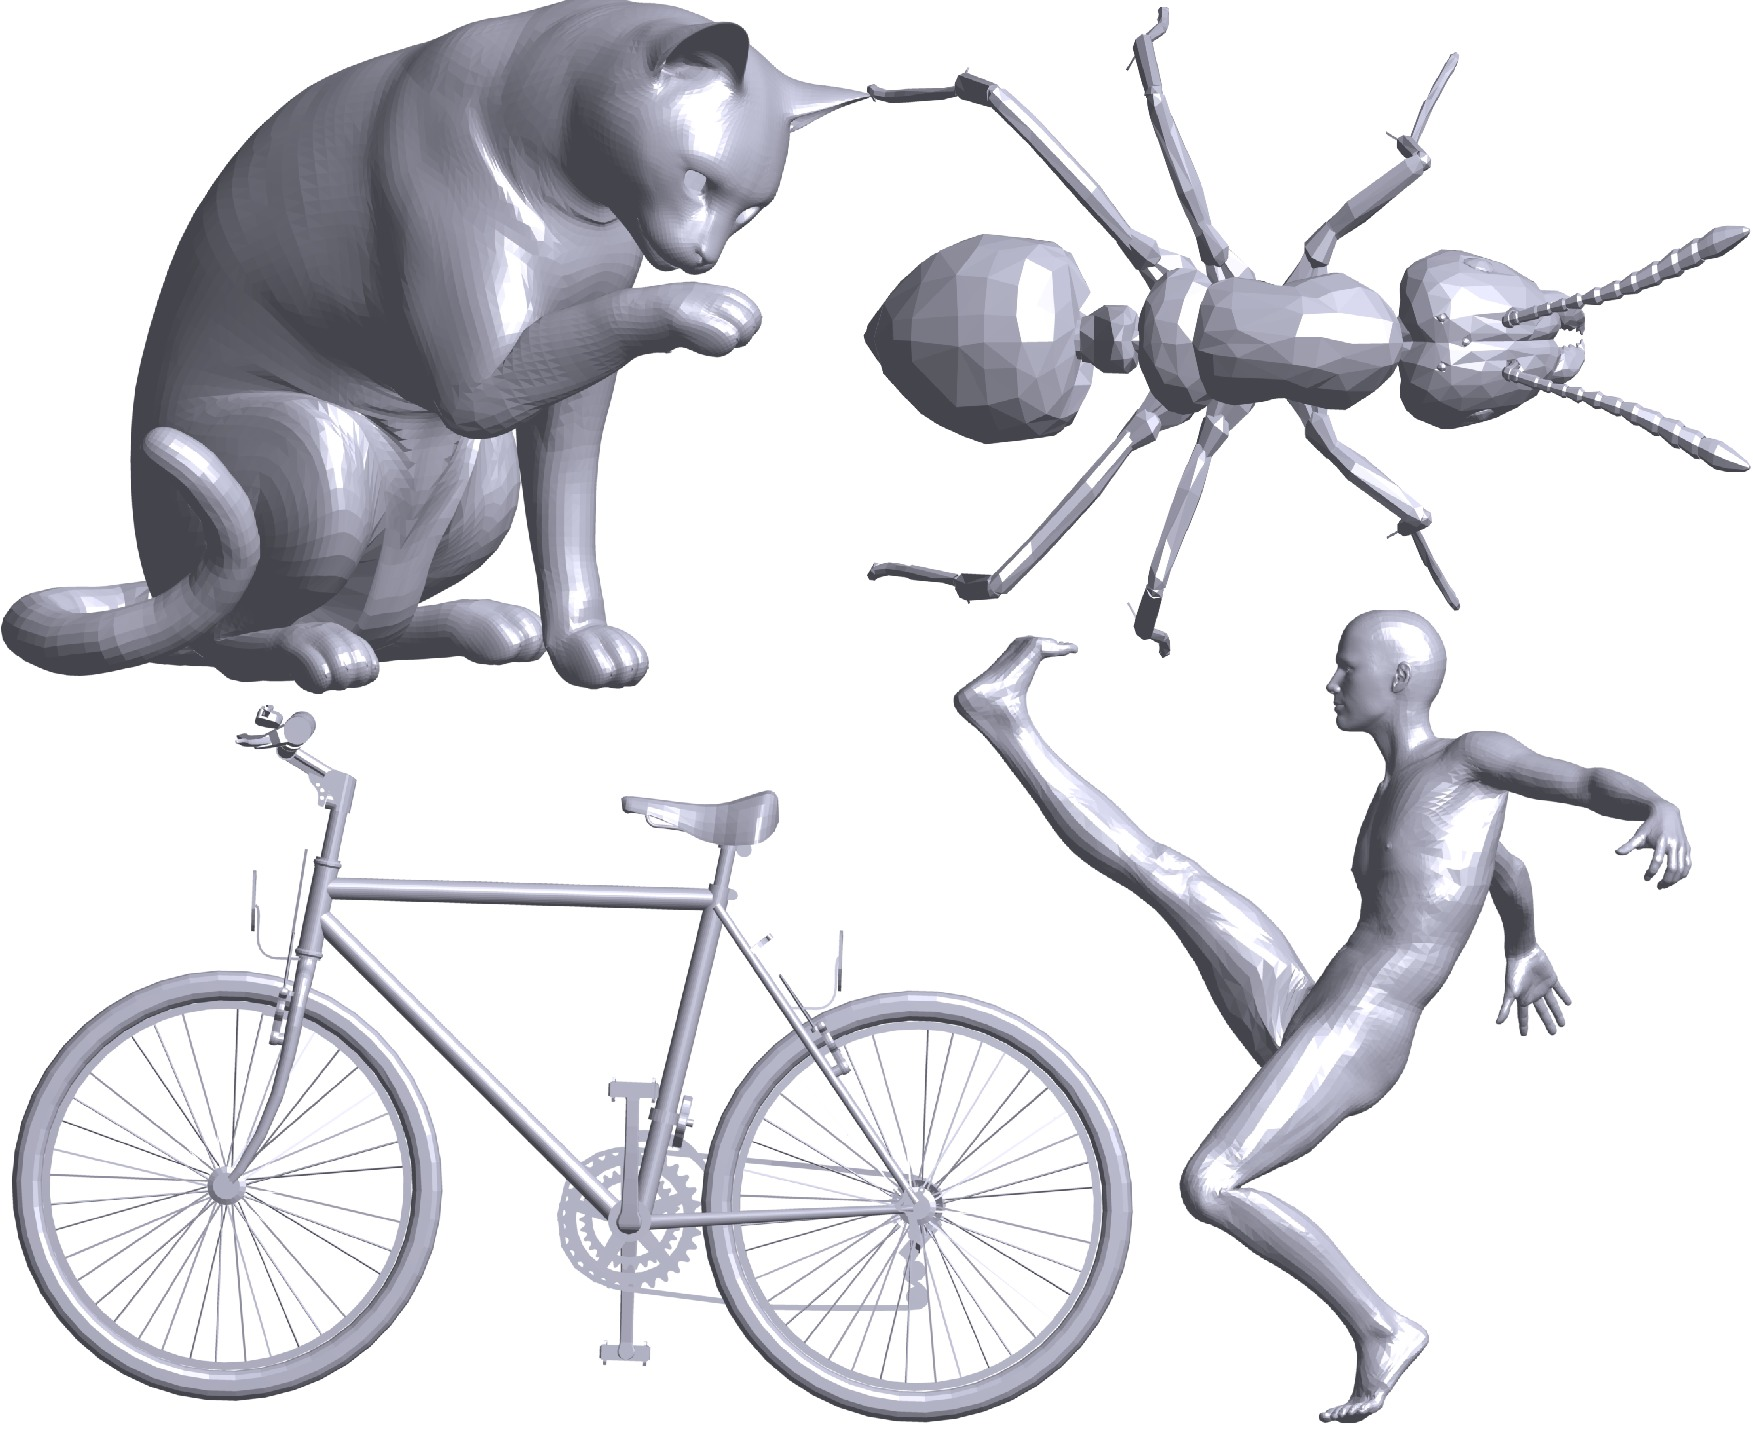
\includegraphics[width=0.75\linewidth]{./fig/eval/sampleshape.pdf}
%\caption{Example shapes taken from the \meshset dataset.} 
%\label{fig/eval/sampleshapes}
%\end{figure}

\begin{figure}
	\begin{subfigure}[t]{0.19\linewidth} \centering
		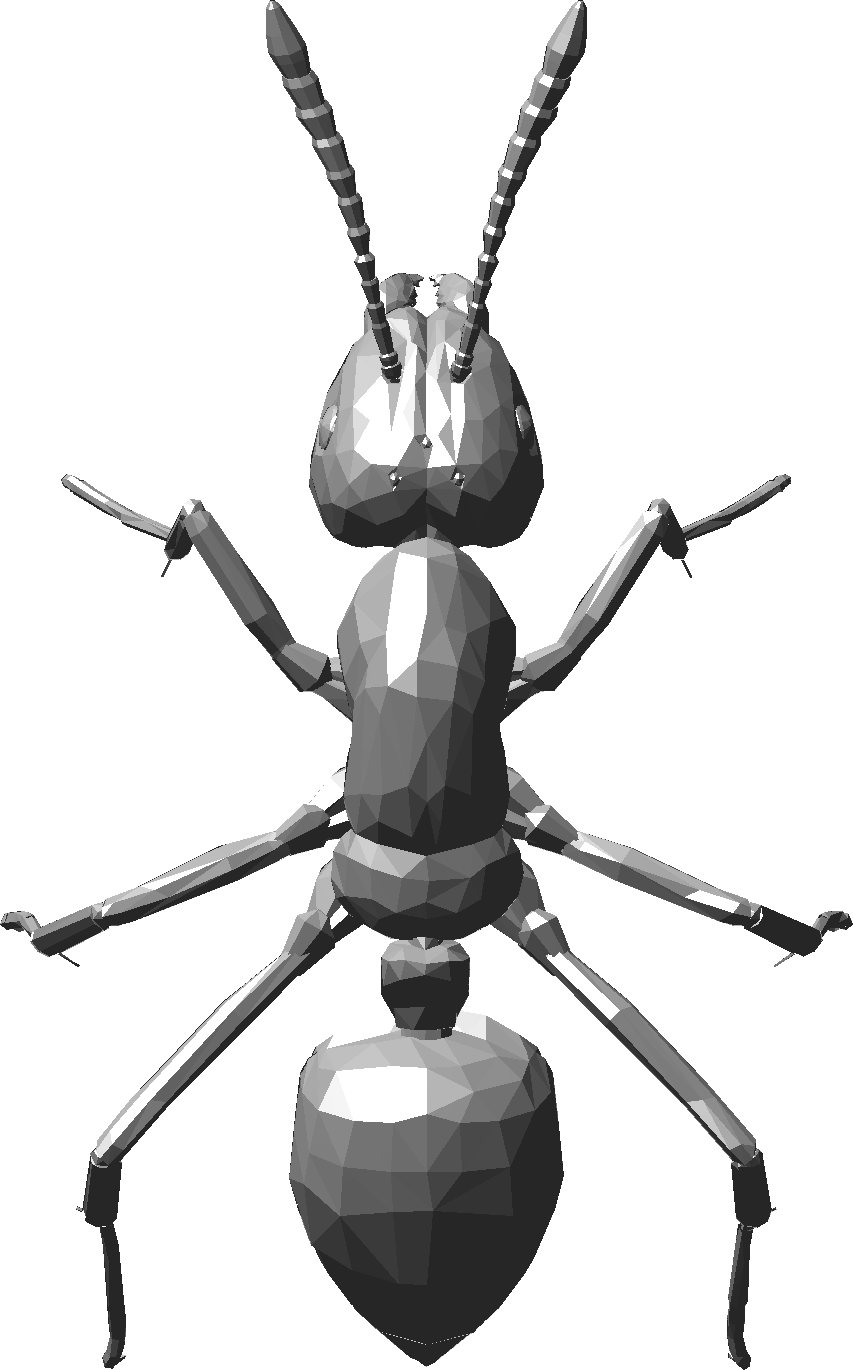
\includegraphics[width=0.7\linewidth]{./fig/eval/01ant.png}  
		\caption{Ant} 	
	\end{subfigure}
	\begin{subfigure}[t]{0.19\linewidth} \centering
		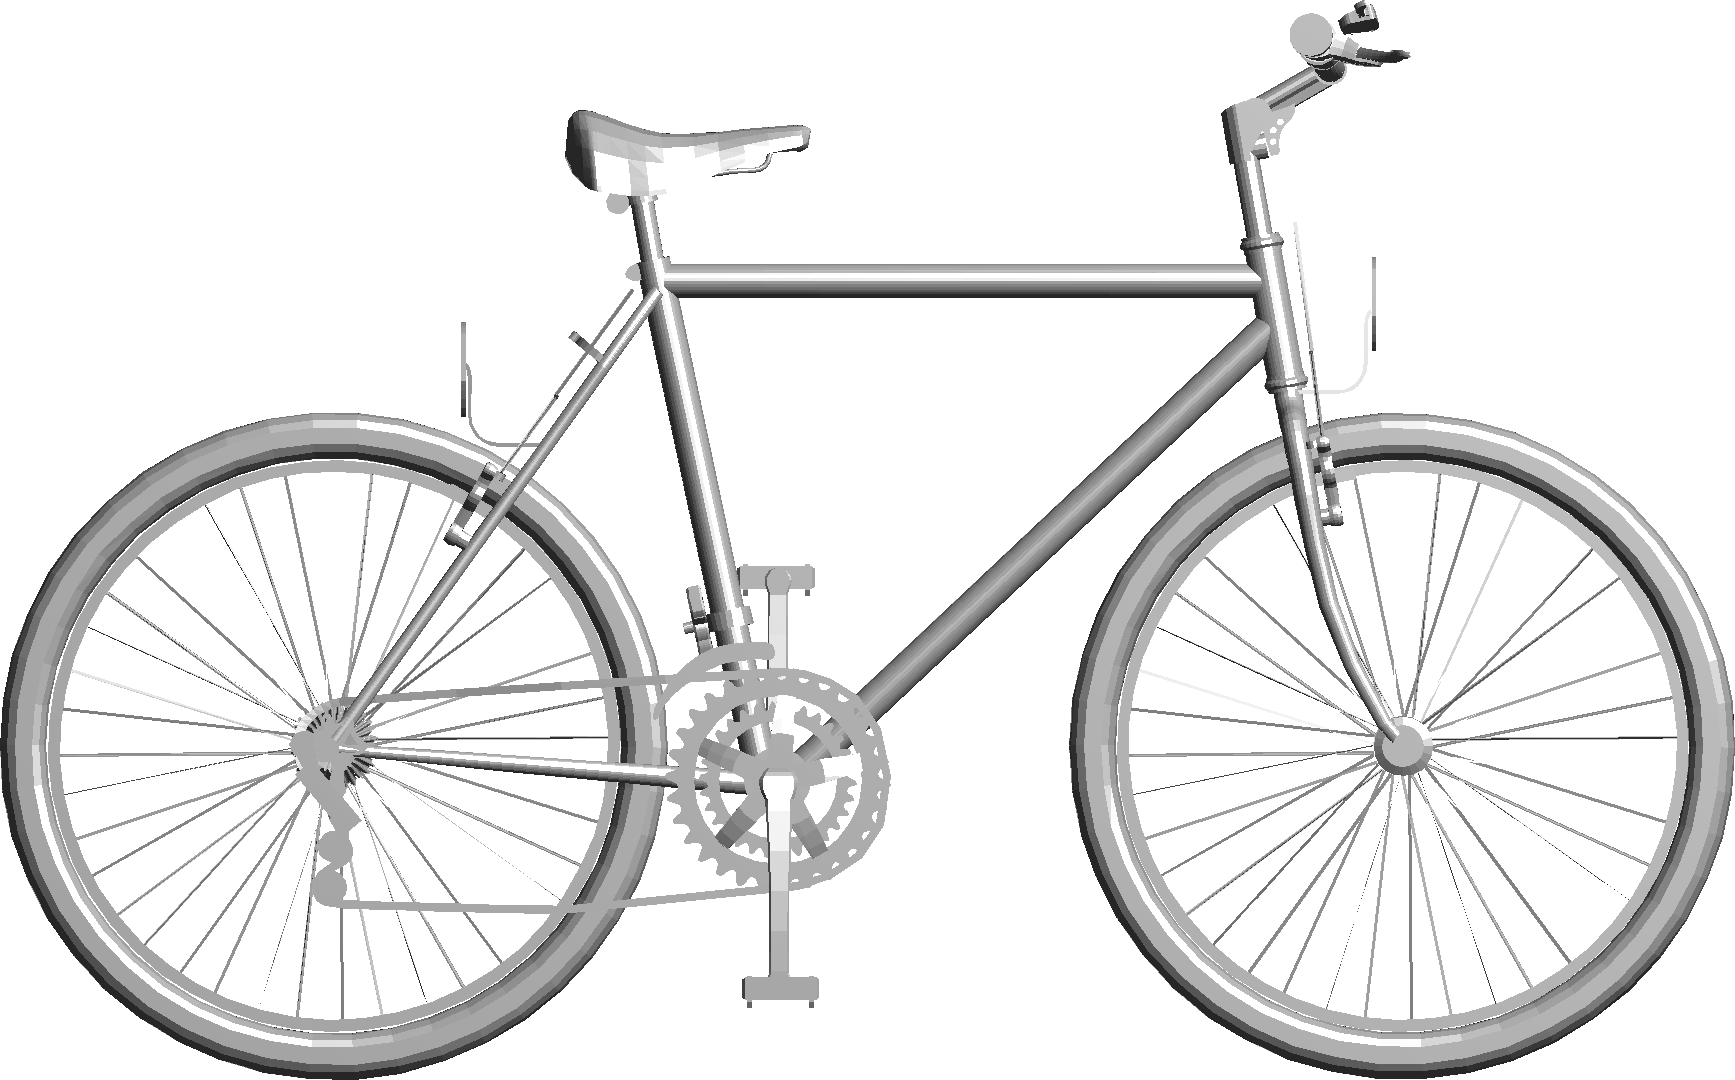
\includegraphics[width=1\linewidth]{./fig/eval/02bicycle.png}  
		\caption{Bicycle} 	
	\end{subfigure}
	\begin{subfigure}[t]{0.19\linewidth} \centering
		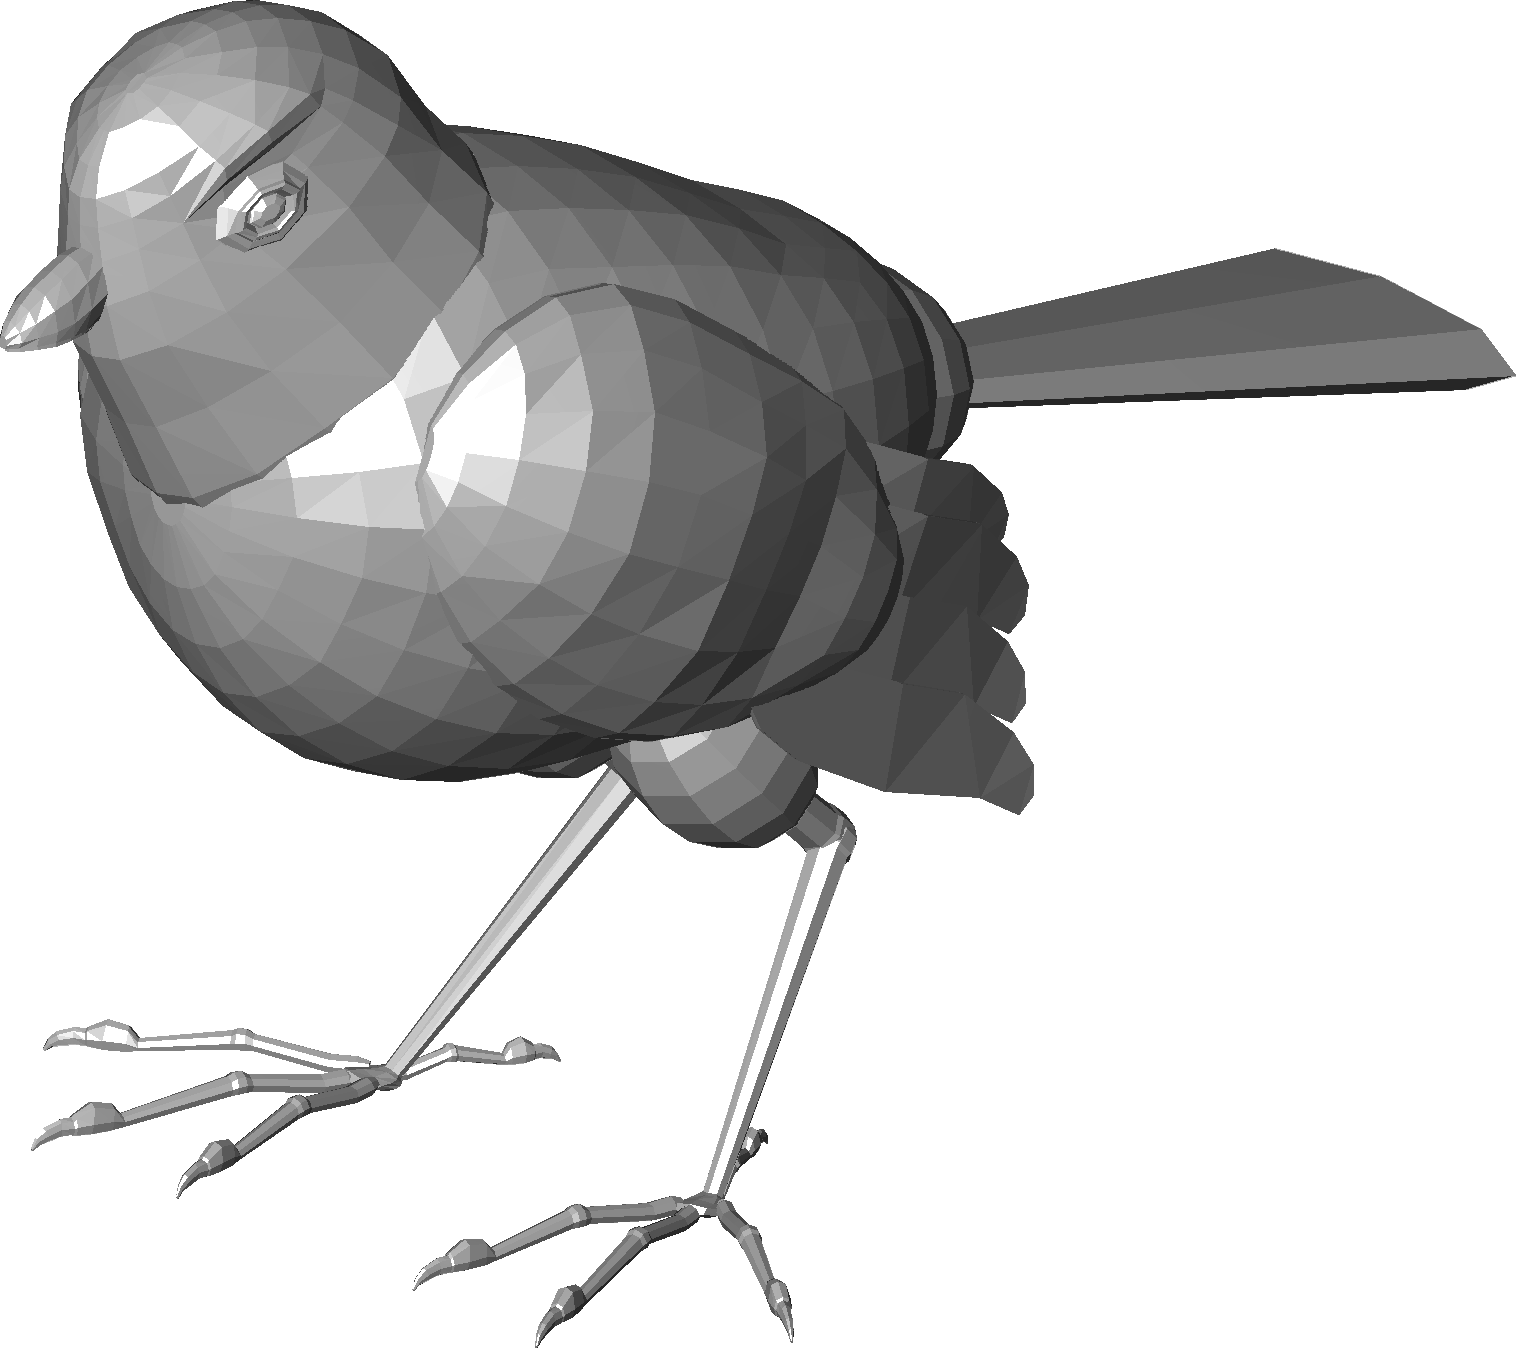
\includegraphics[width=1\linewidth]{./fig/eval/03bird.png}  
		\caption{Bird} 	
	\end{subfigure}
	\begin{subfigure}[t]{0.19\linewidth} \centering
		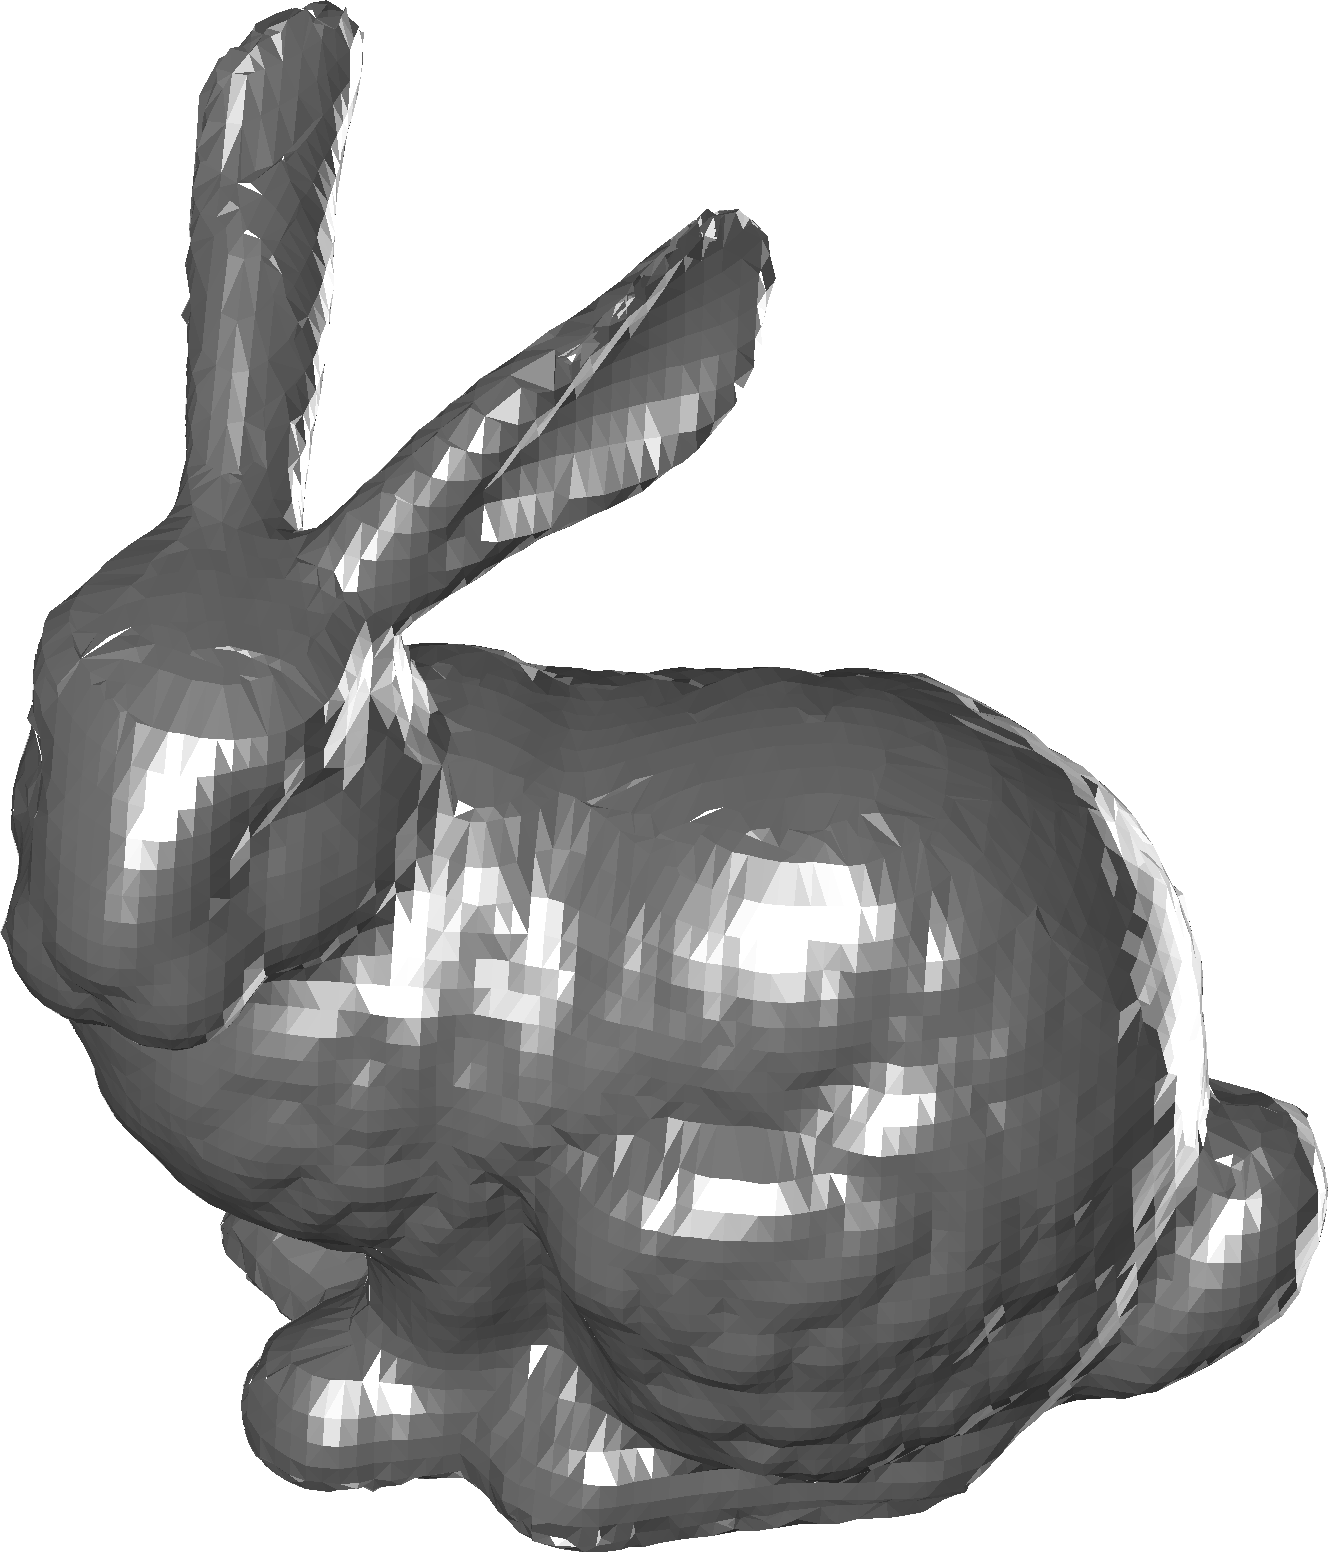
\includegraphics[width=0.9\linewidth]{./fig/eval/04bunny.png}  
		\caption{Bunny} 	
	\end{subfigure} 
	\begin{subfigure}[t]{0.19\linewidth} \centering
		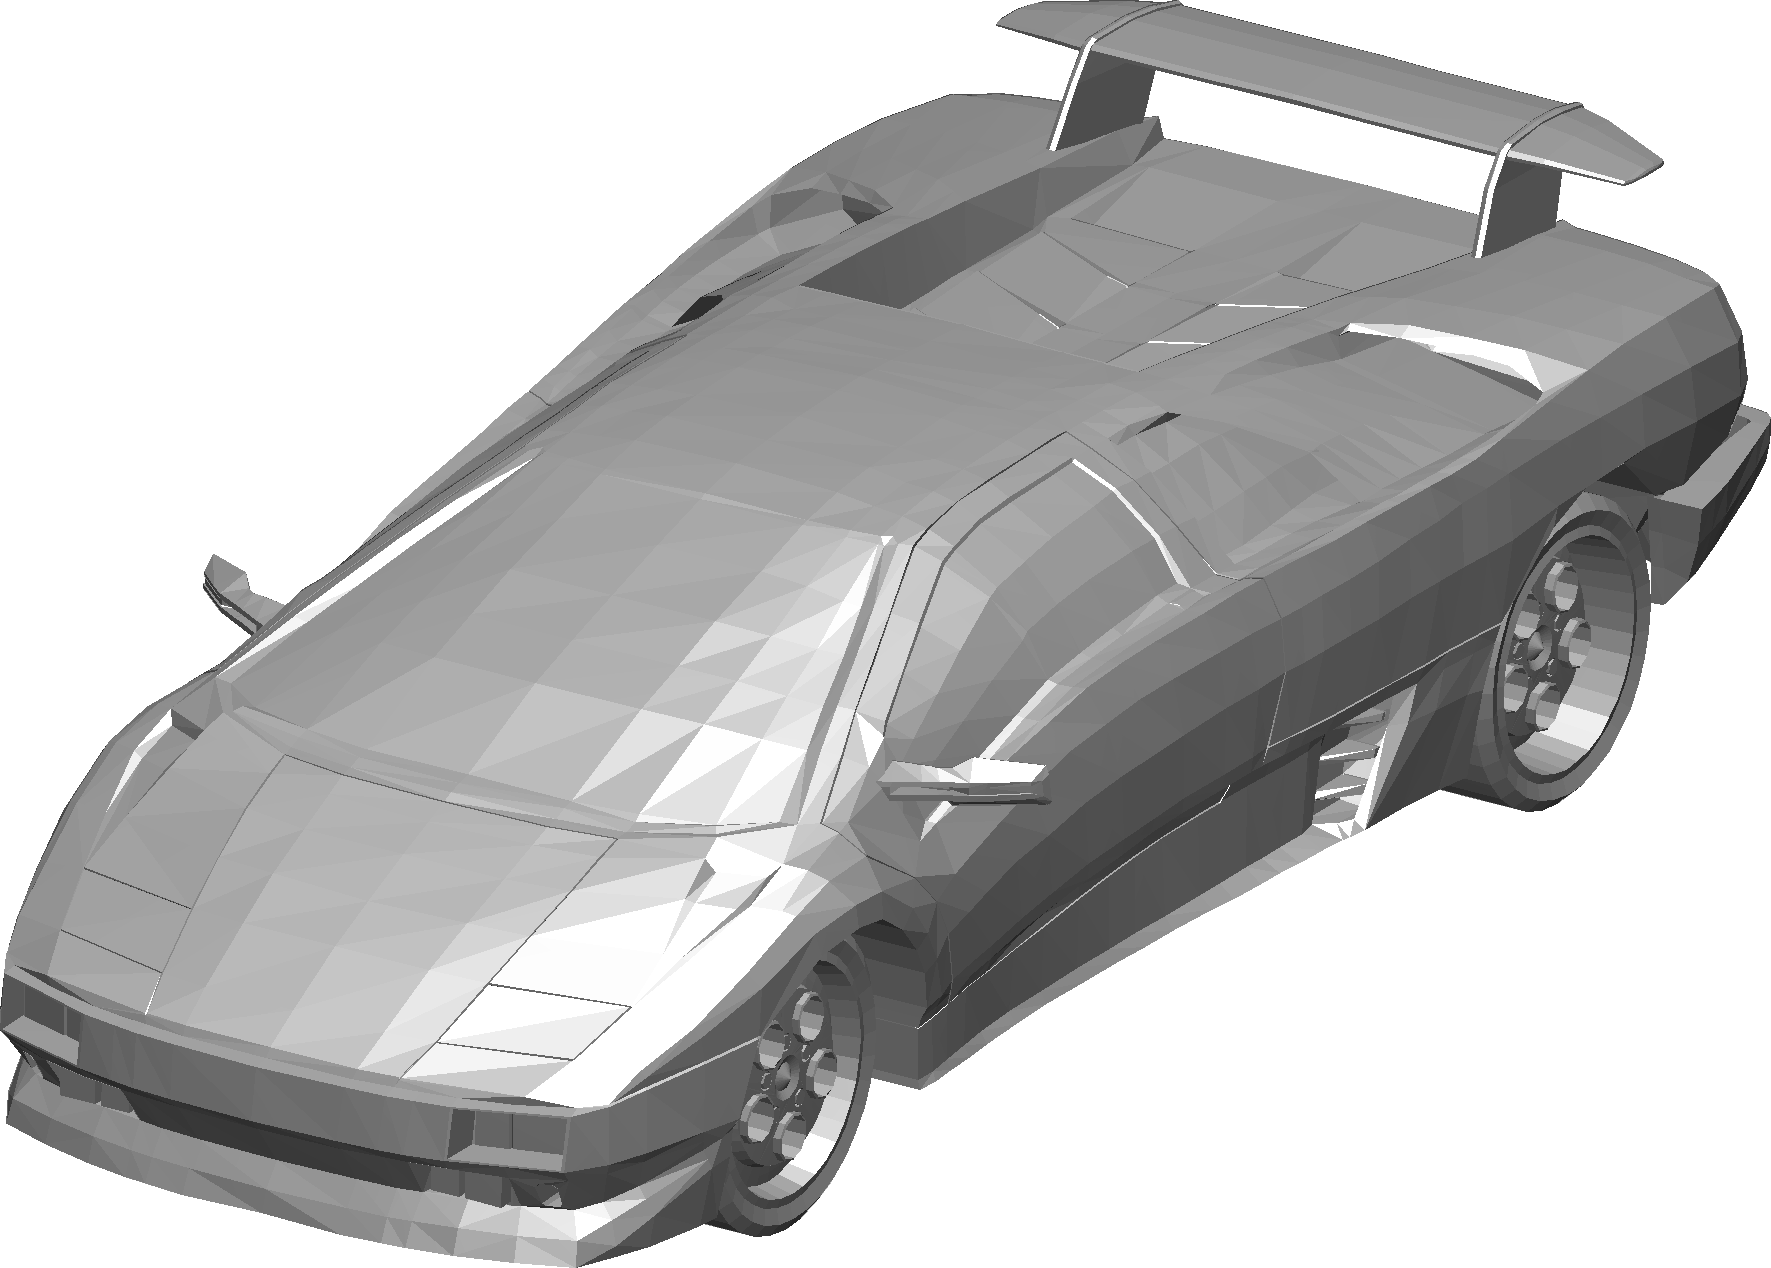
\includegraphics[width=1\linewidth]{./fig/eval/05car.png}  
		\caption{Car} 	
	\end{subfigure} \\ 
	\begin{subfigure}[t]{0.19\linewidth} \centering
		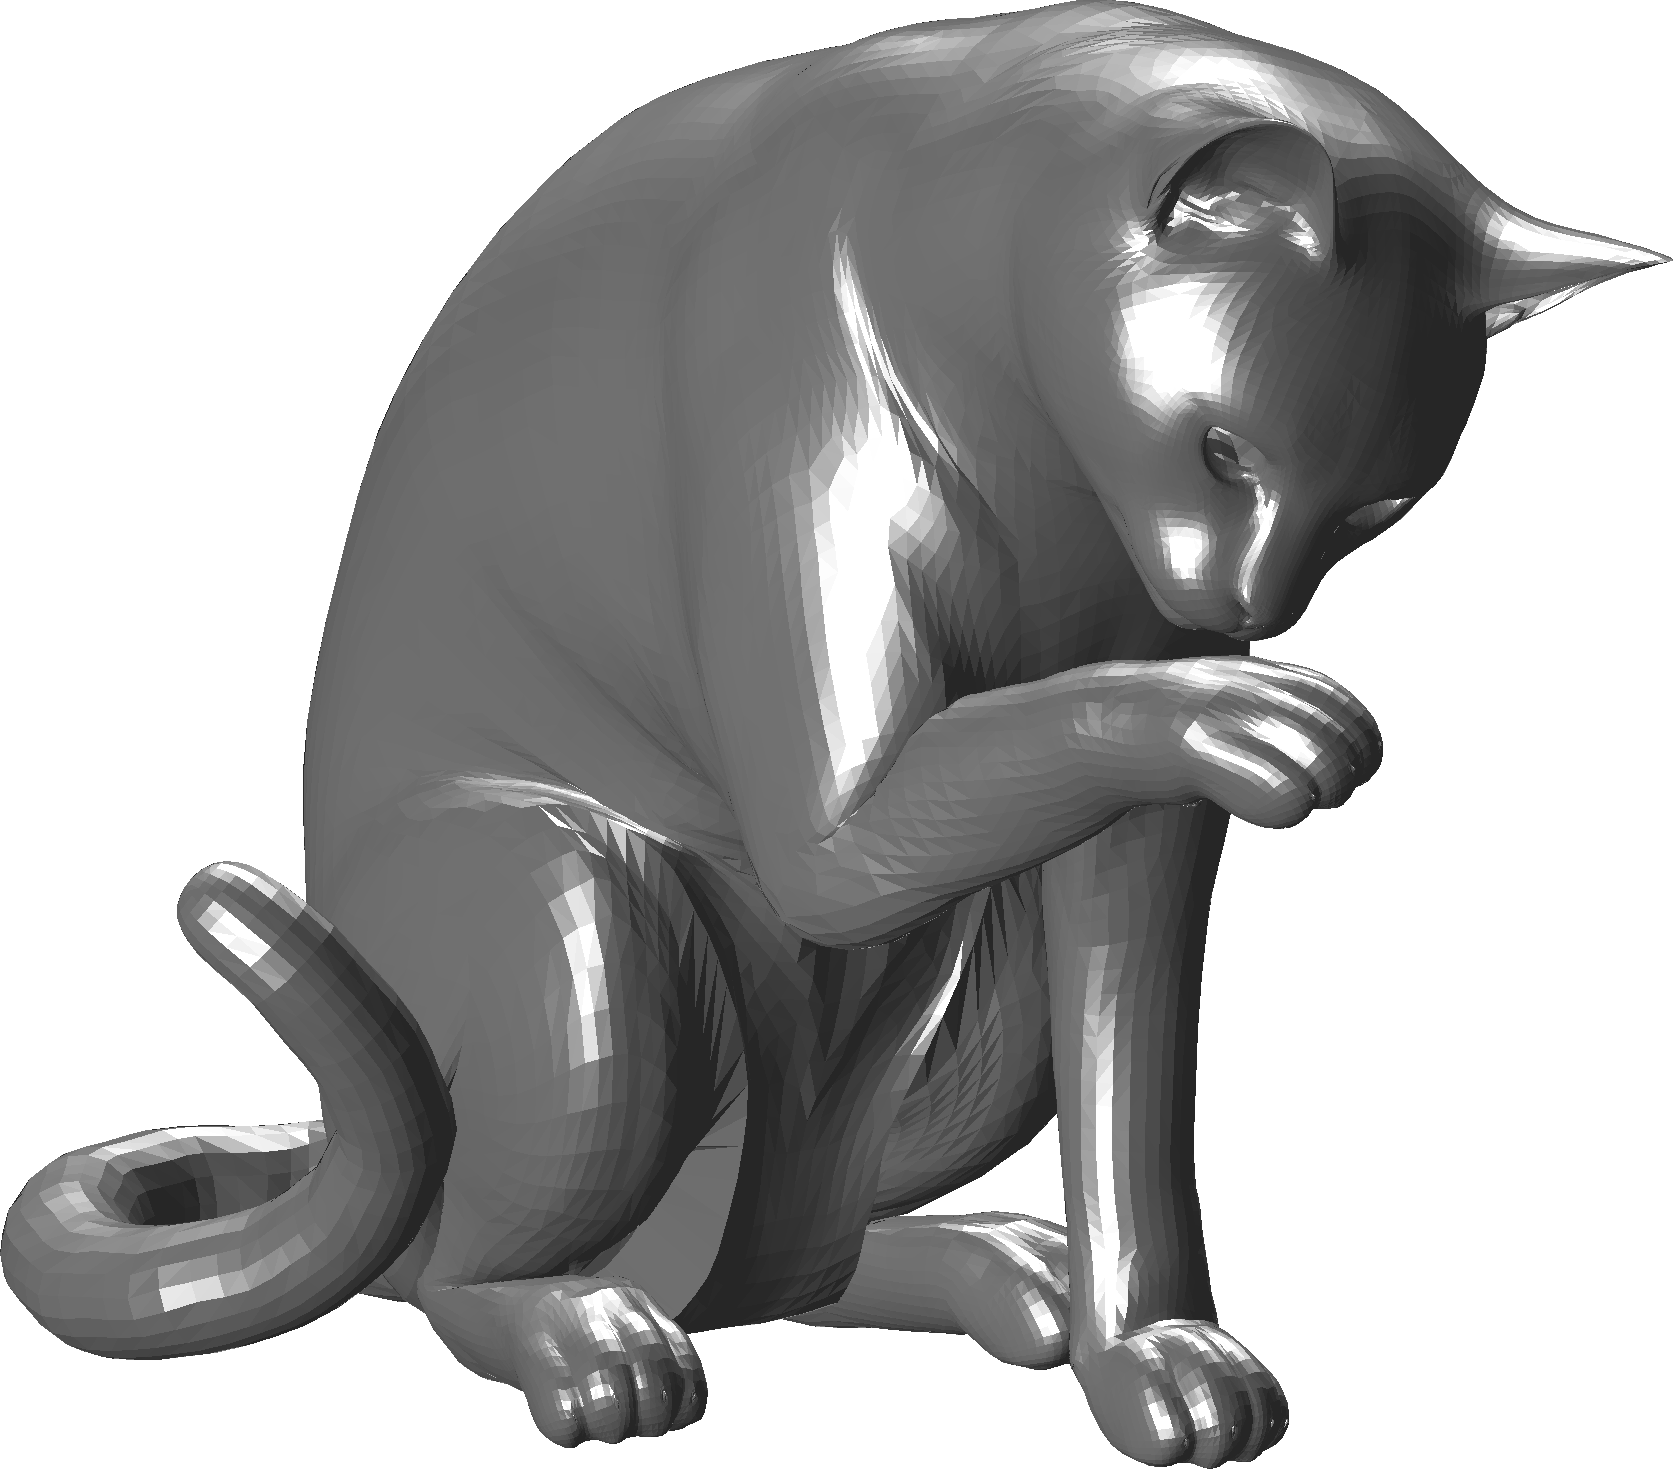
\includegraphics[width=1\linewidth]{./fig/eval/06cat.png}  
		\caption{Cat} 	
	\end{subfigure}
	\begin{subfigure}[t]{0.19\linewidth} \centering
		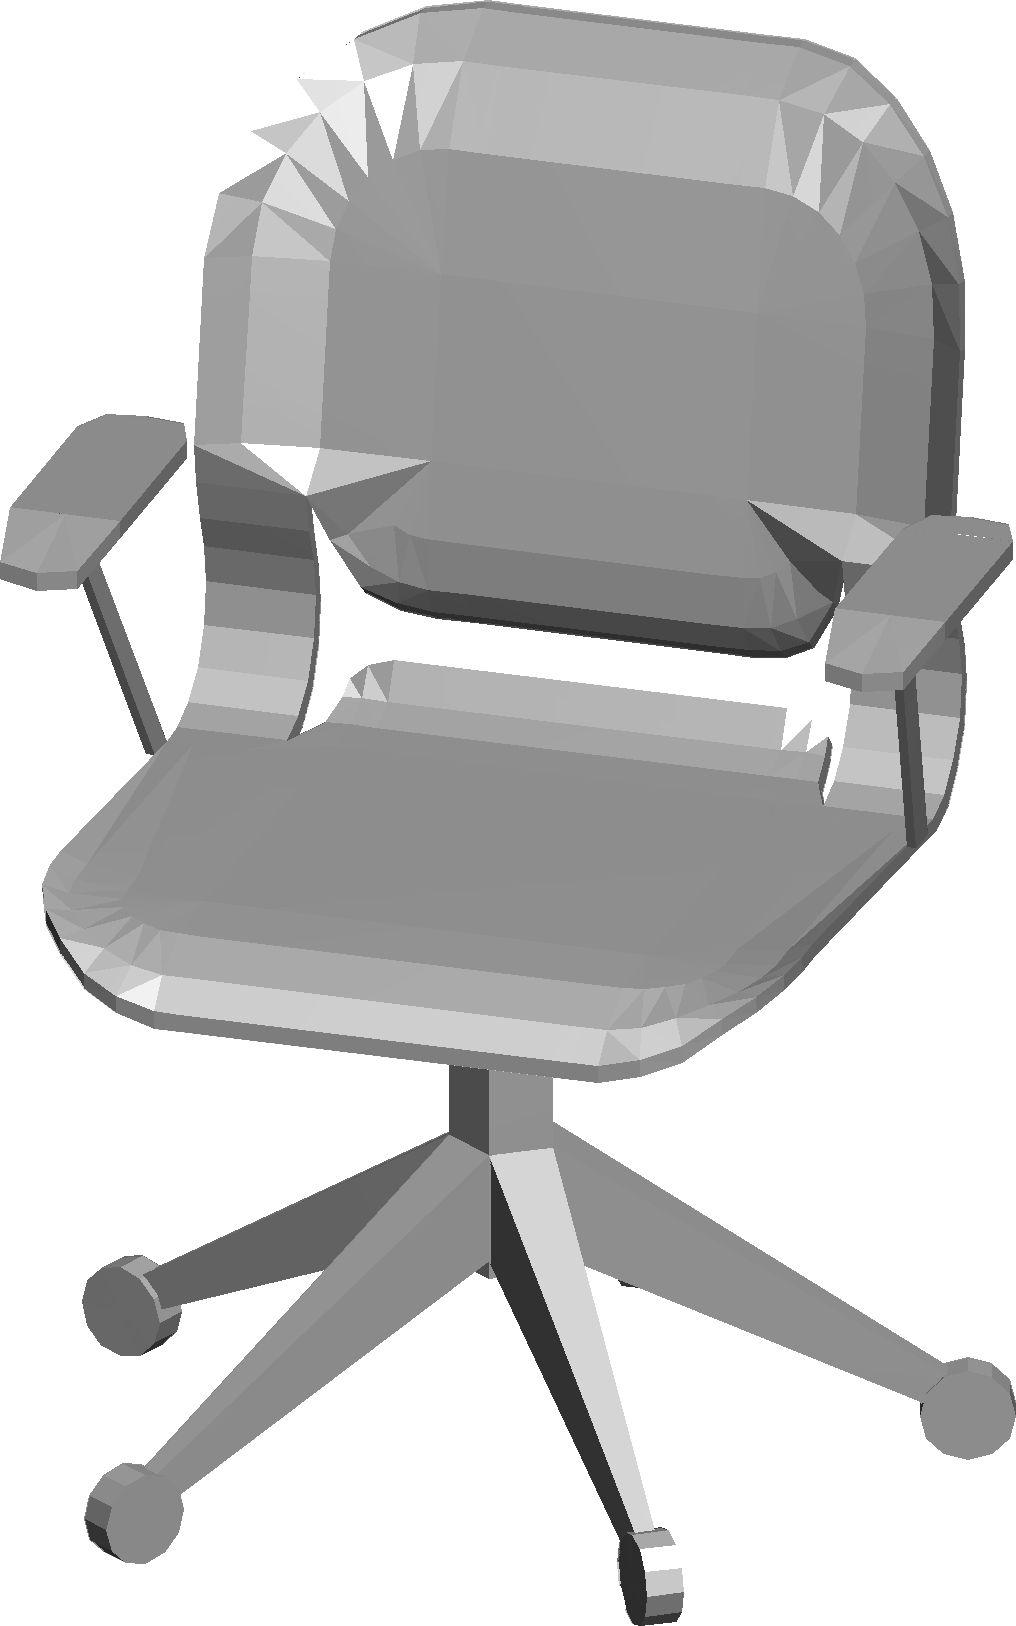
\includegraphics[width=0.7\linewidth]{./fig/eval/07chair.png}  
		\caption{Chair} 	
	\end{subfigure}
	\begin{subfigure}[t]{0.19\linewidth} \centering
		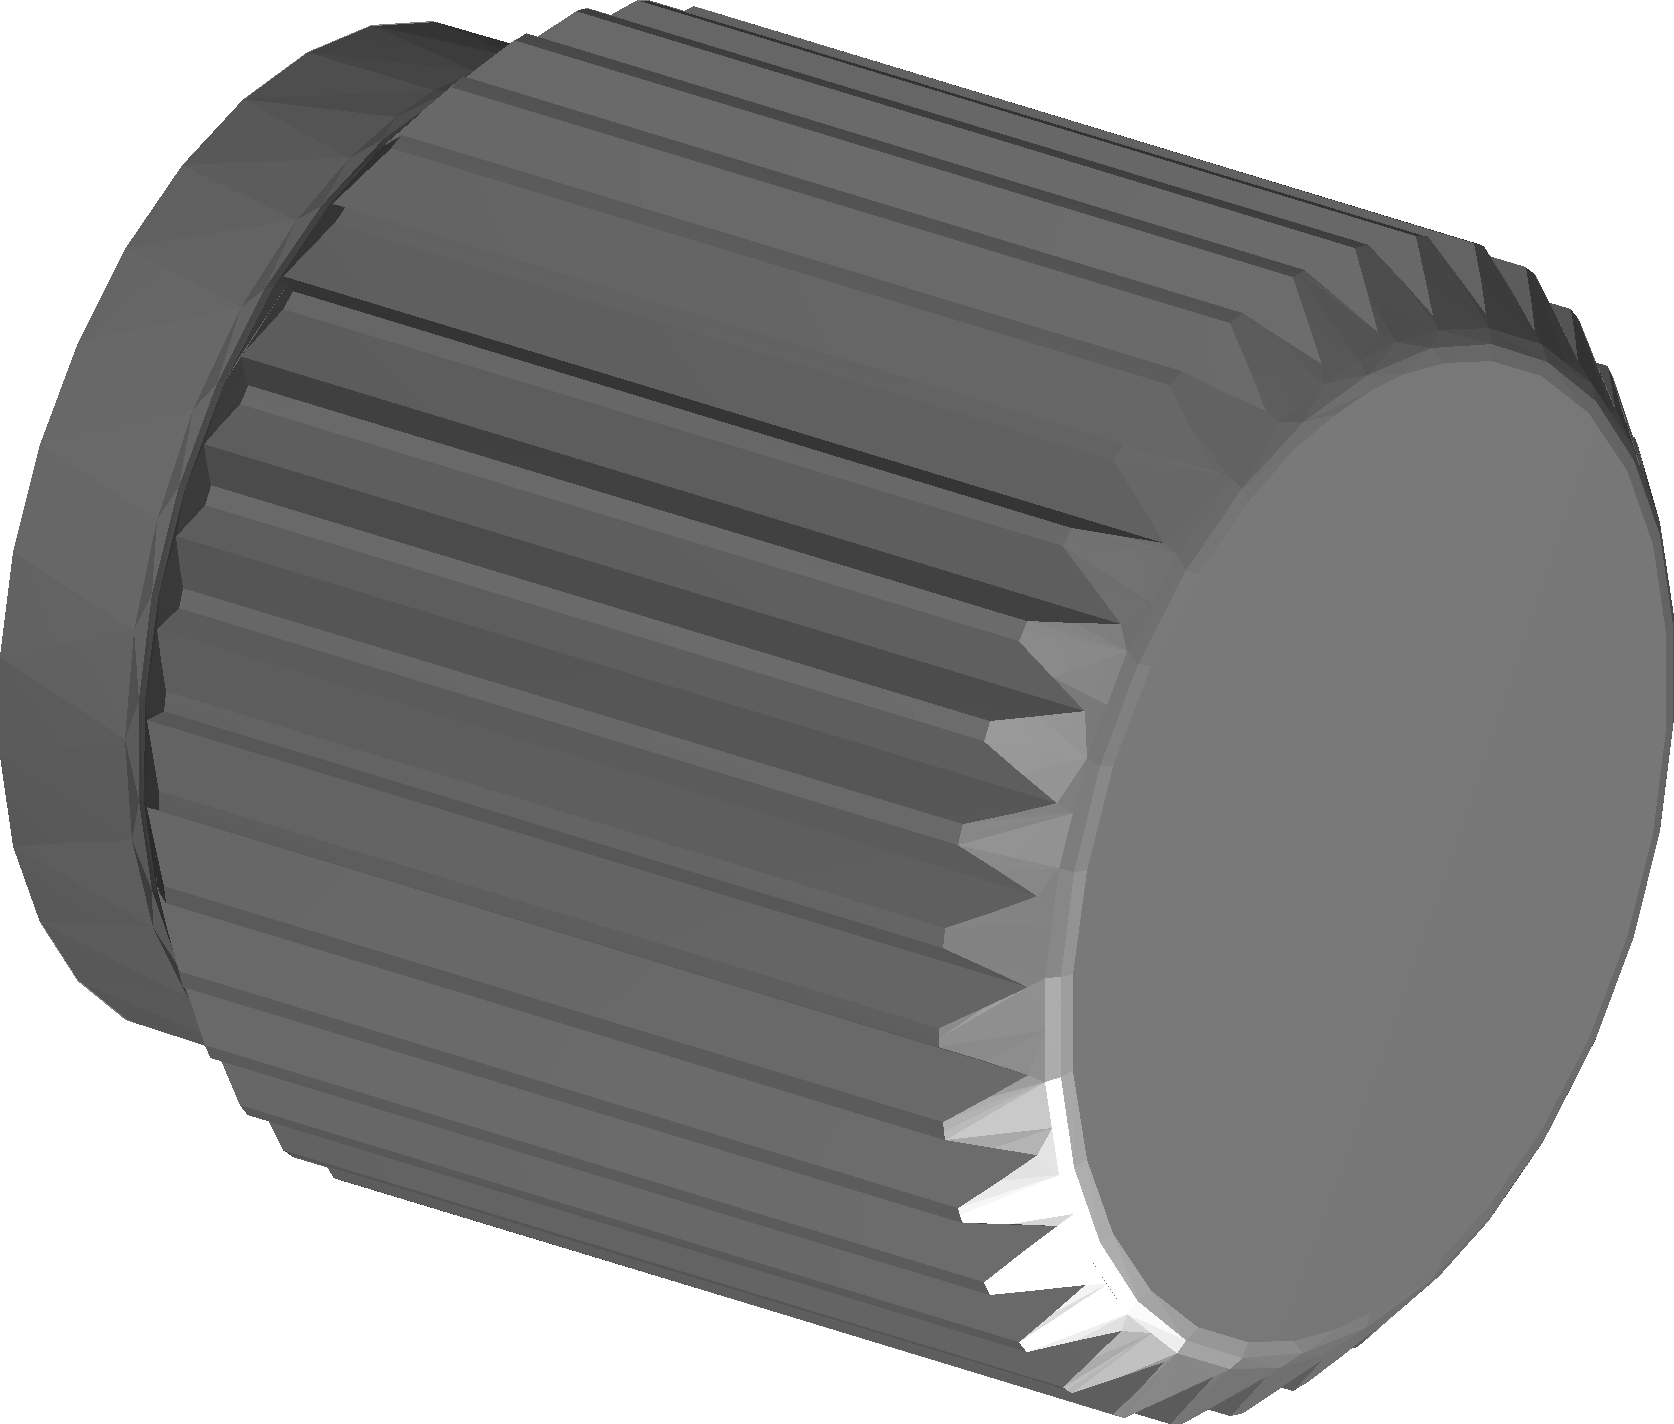
\includegraphics[width=1\linewidth]{./fig/eval/08cog.png}  
		\caption{Cog} 	
	\end{subfigure}
	\begin{subfigure}[t]{0.19\linewidth} \centering
		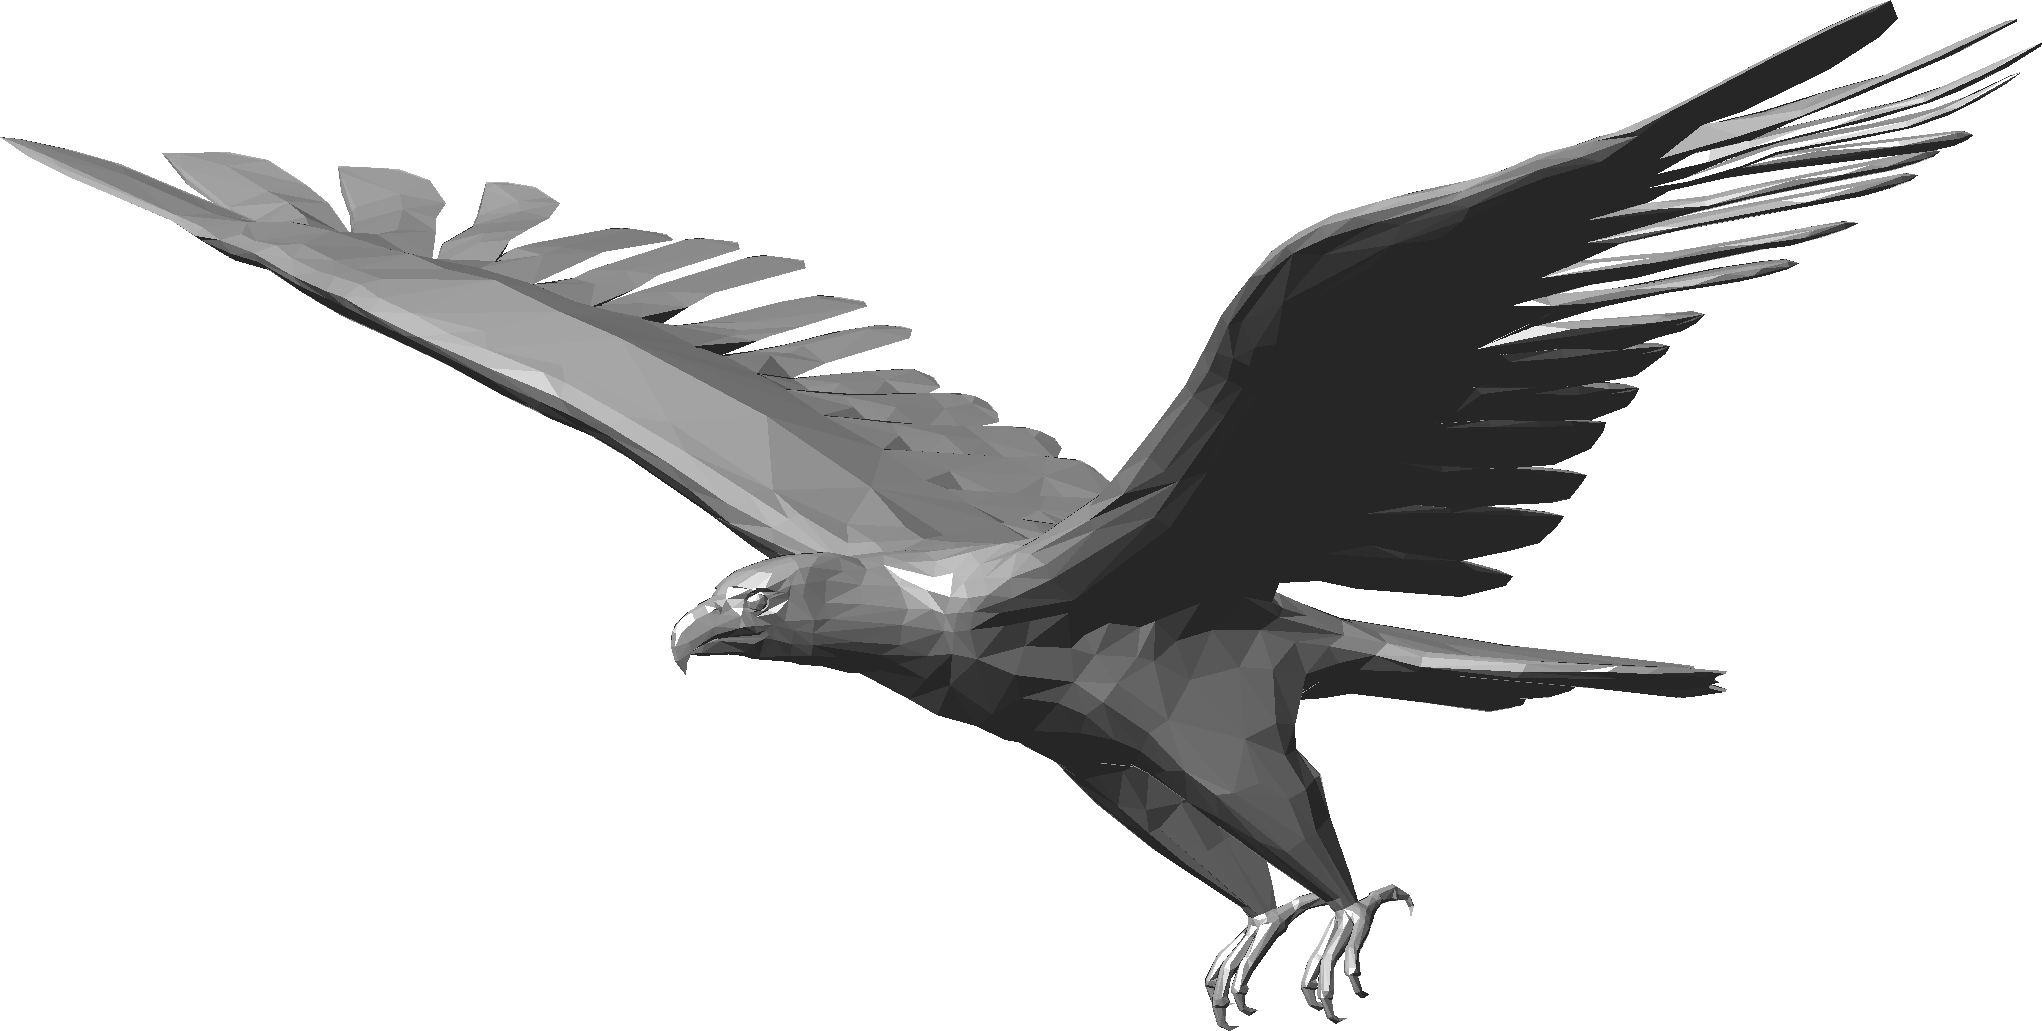
\includegraphics[width=1\linewidth]{./fig/eval/09eagle.png}  
		\caption{Eagle} 	
	\end{subfigure} 
	\begin{subfigure}[t]{0.19\linewidth} \centering
		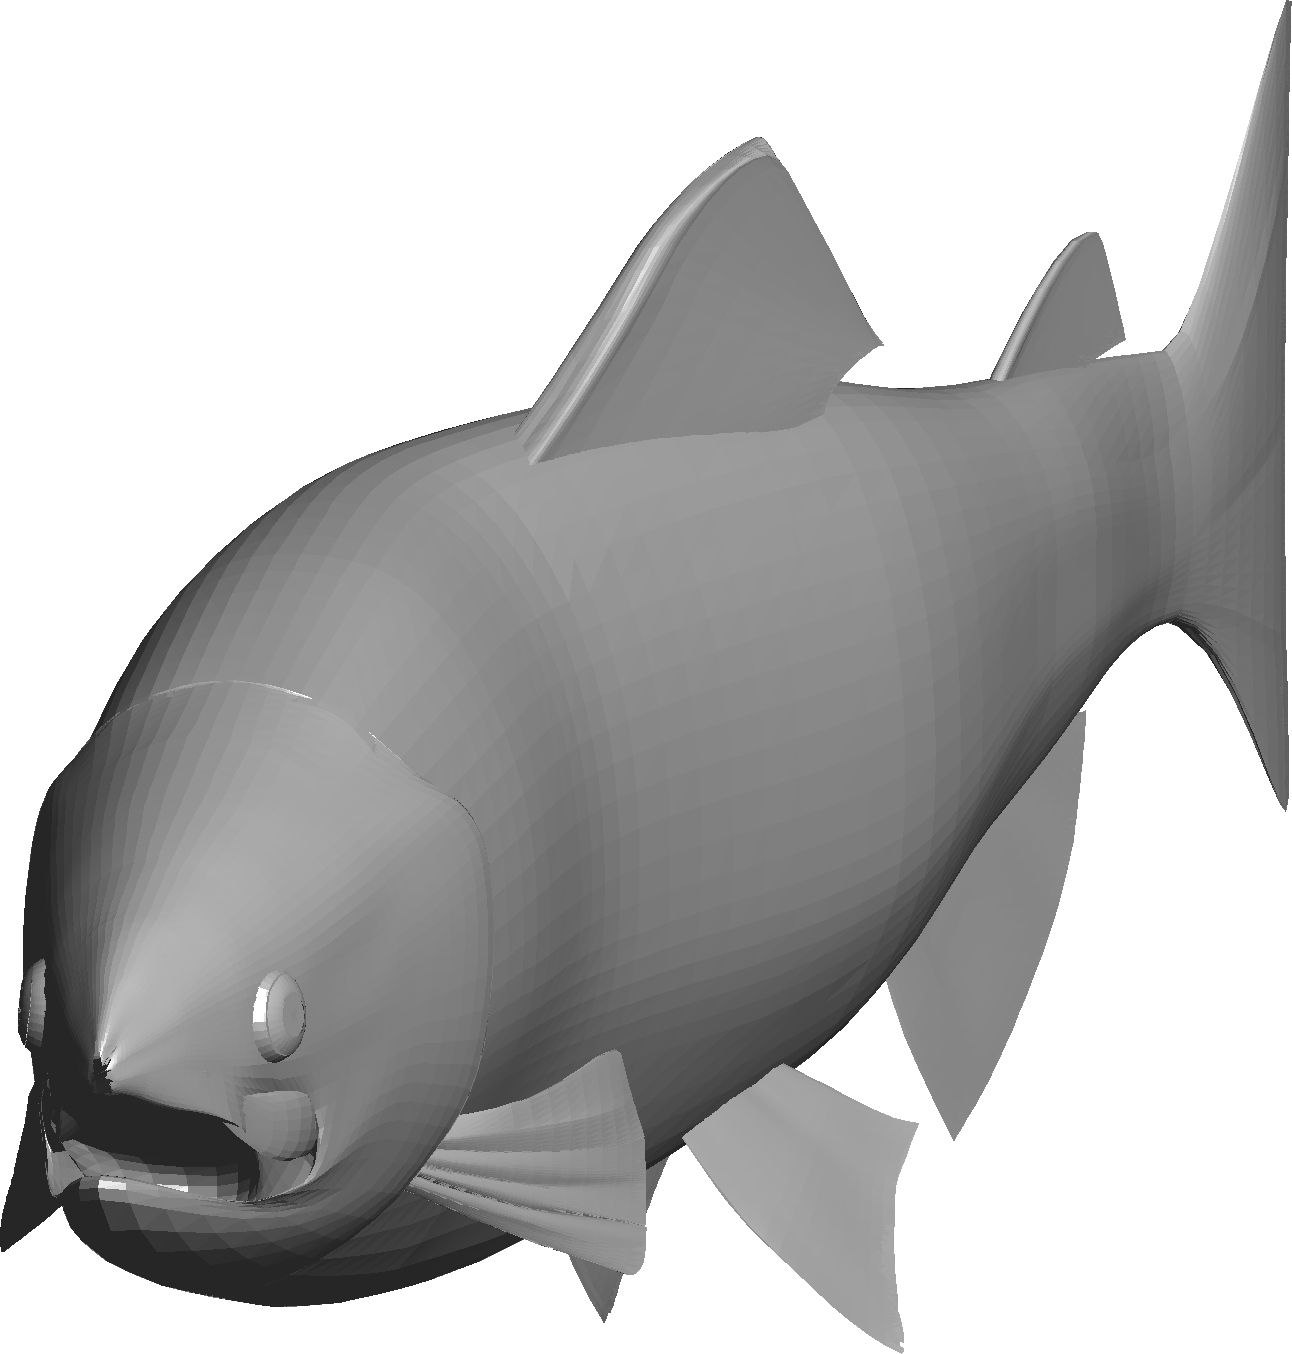
\includegraphics[width=1\linewidth]{./fig/eval/10fish.png}  
		\caption{Fish} 	
	\end{subfigure} \\ 
	\begin{subfigure}[t]{0.19\linewidth} \centering
		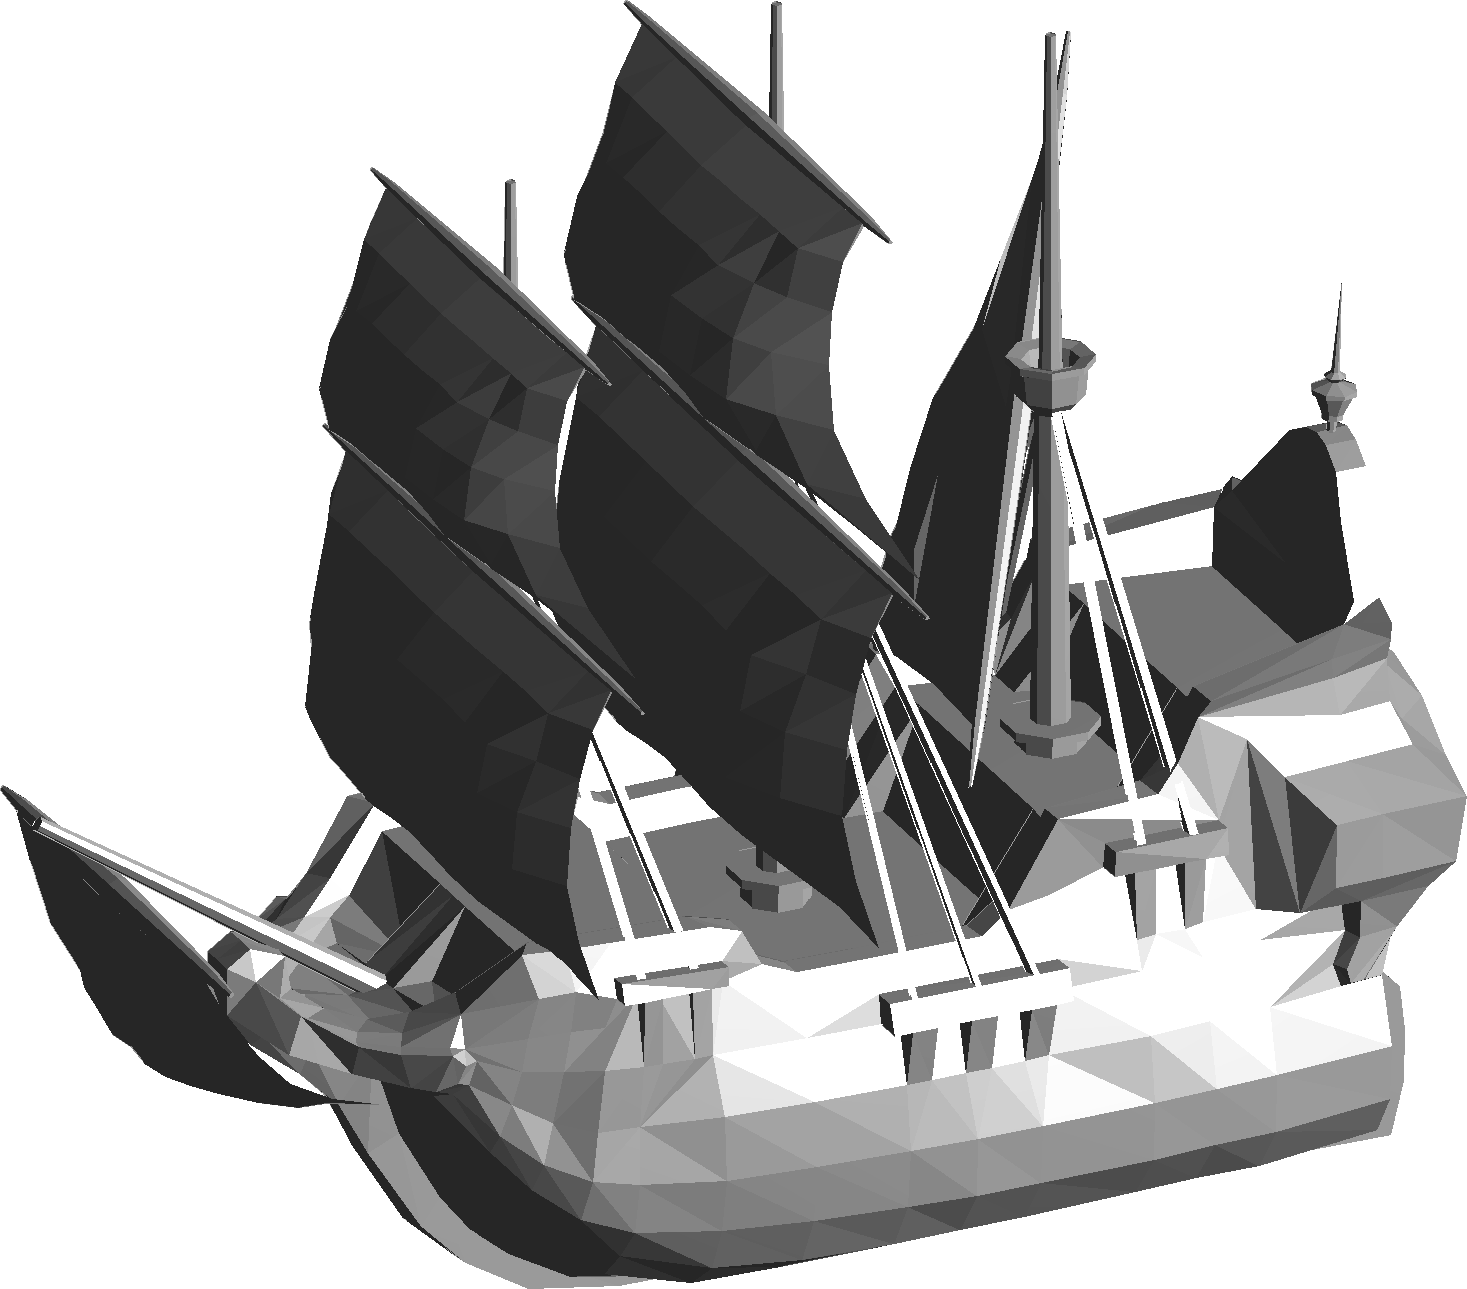
\includegraphics[width=1\linewidth]{./fig/eval/11galleon.png}  
		\caption{Galleon} 	
	\end{subfigure}
	\begin{subfigure}[t]{0.19\linewidth} \centering
		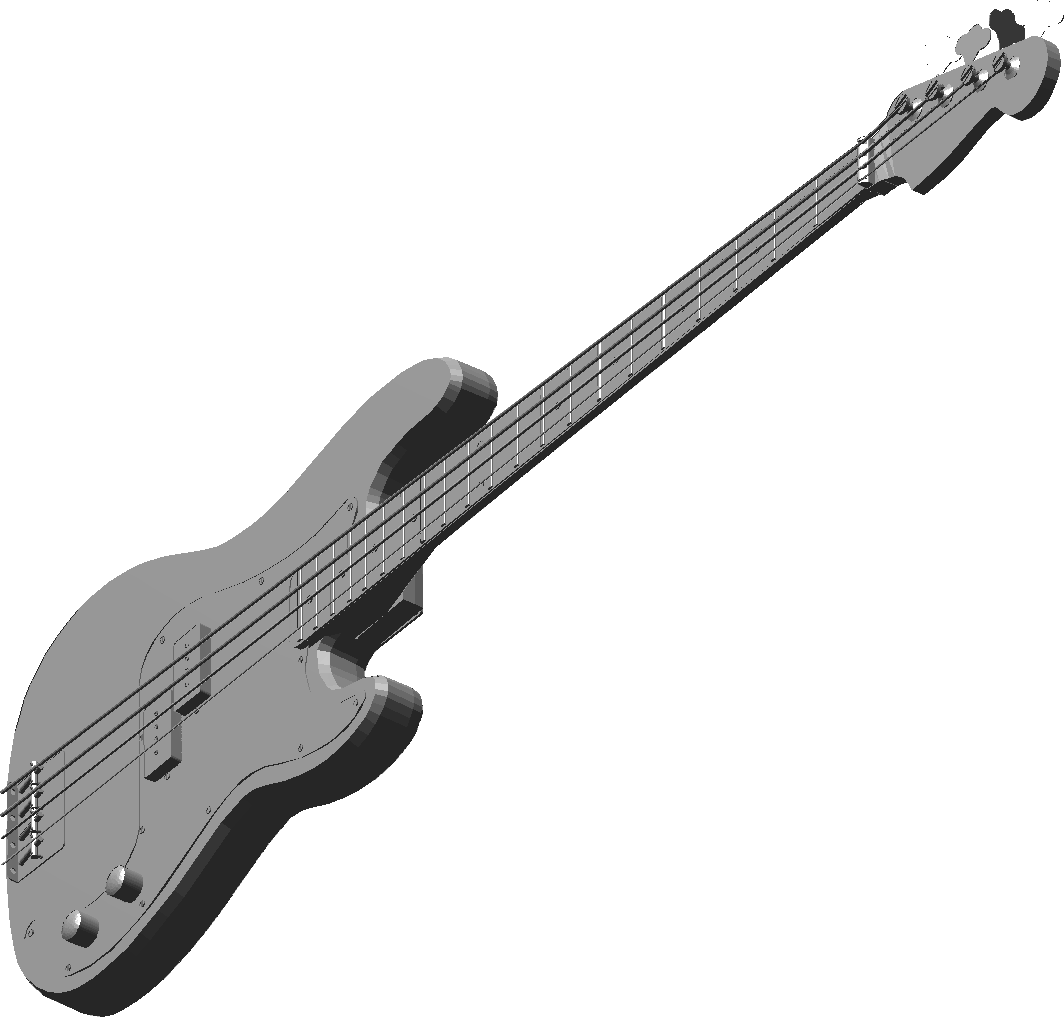
\includegraphics[width=1\linewidth]{./fig/eval/12guitar.png}  
		\caption{Guitar} 	
	\end{subfigure}
	\begin{subfigure}[t]{0.19\linewidth} \centering
		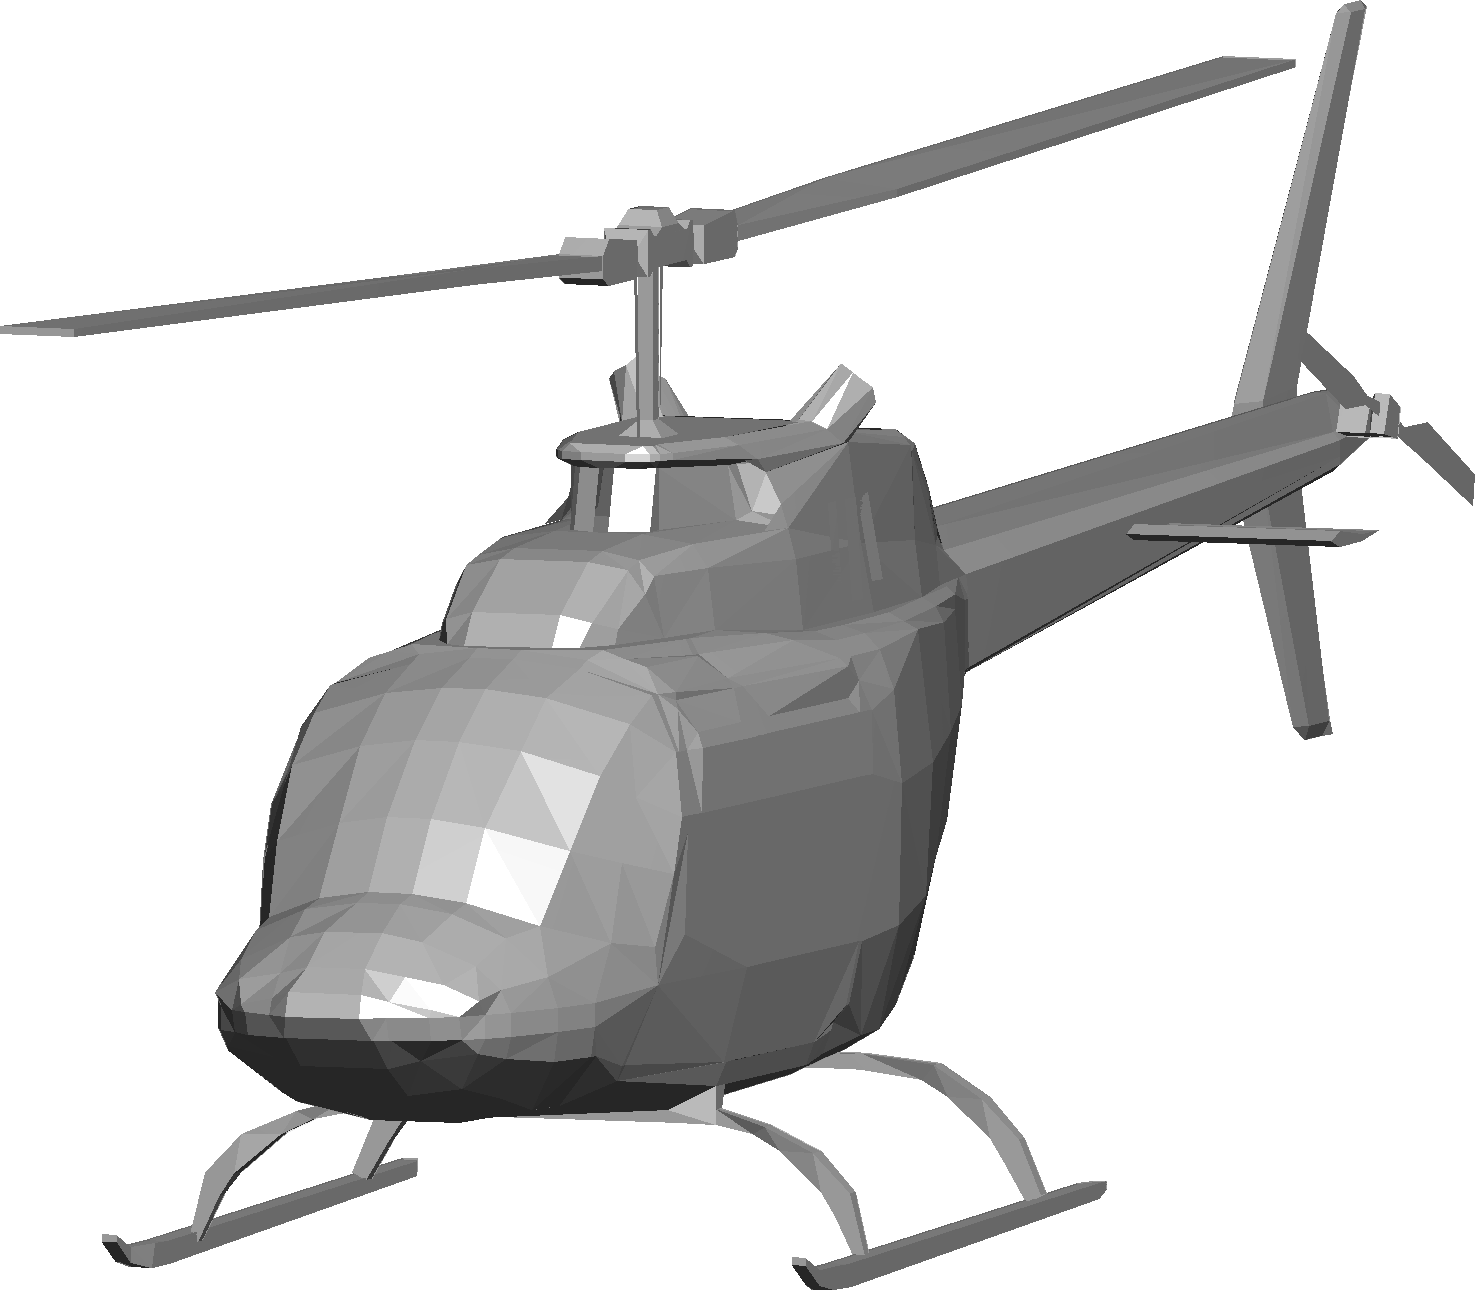
\includegraphics[width=1\linewidth]{./fig/eval/13helicopter.png}  
		\caption{Helicopter} 	
	\end{subfigure}
	\begin{subfigure}[t]{0.19\linewidth} \centering
		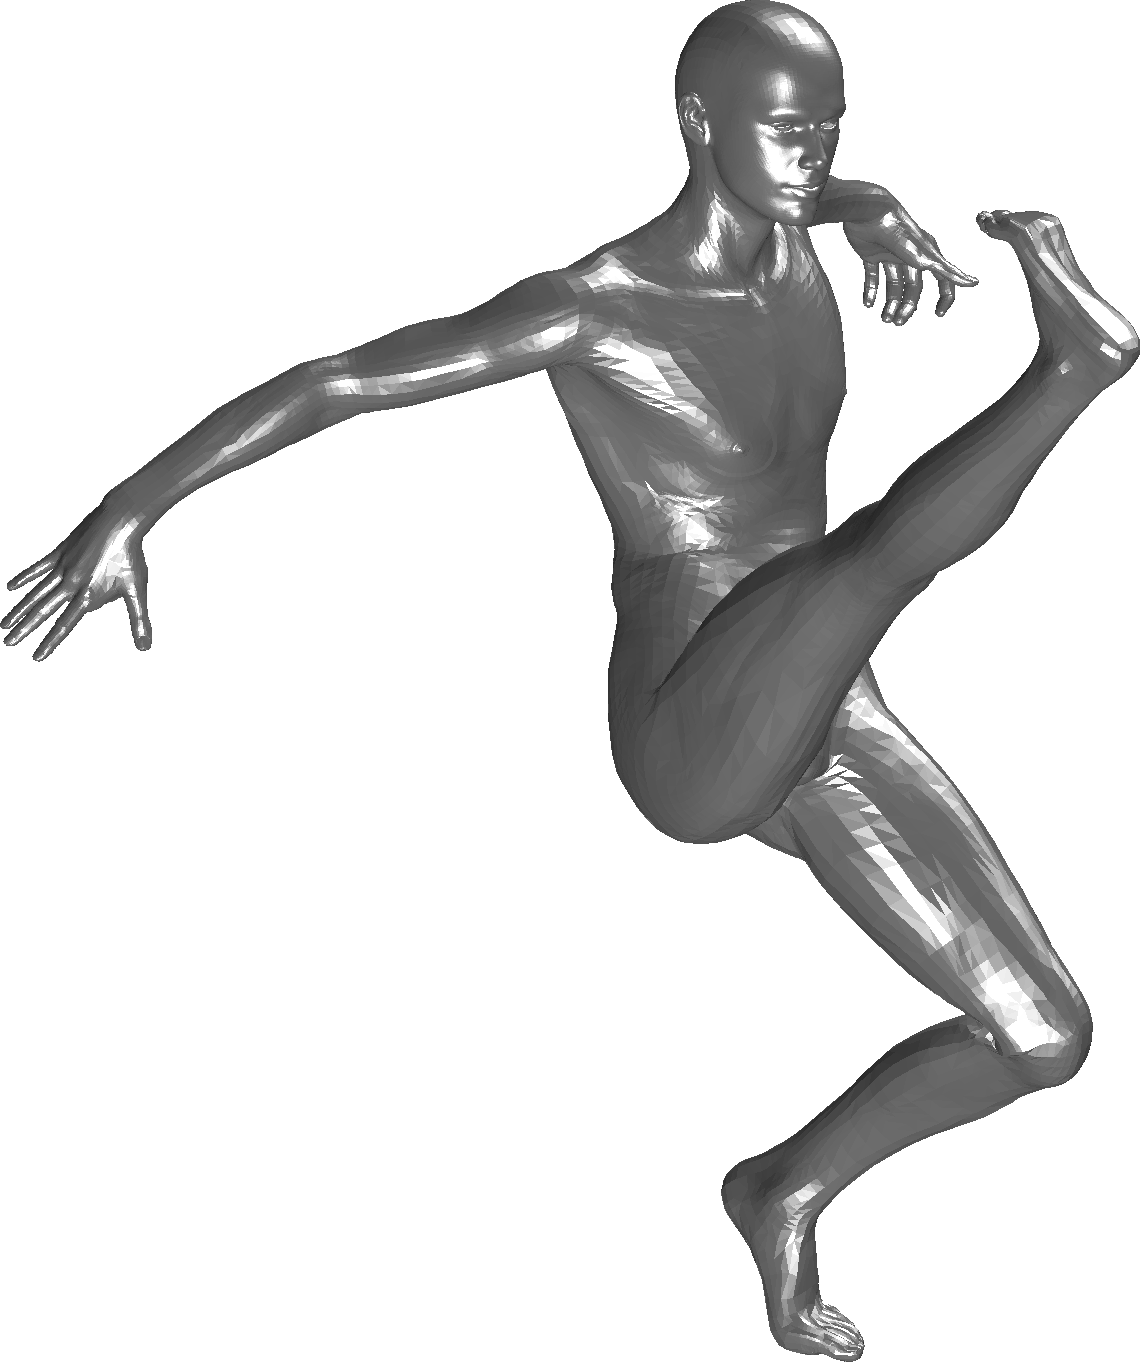
\includegraphics[width=0.8\linewidth]{./fig/eval/14man.png}  
		\caption{Kicking man} 	
	\end{subfigure} 
	\begin{subfigure}[t]{0.19\linewidth} \centering
		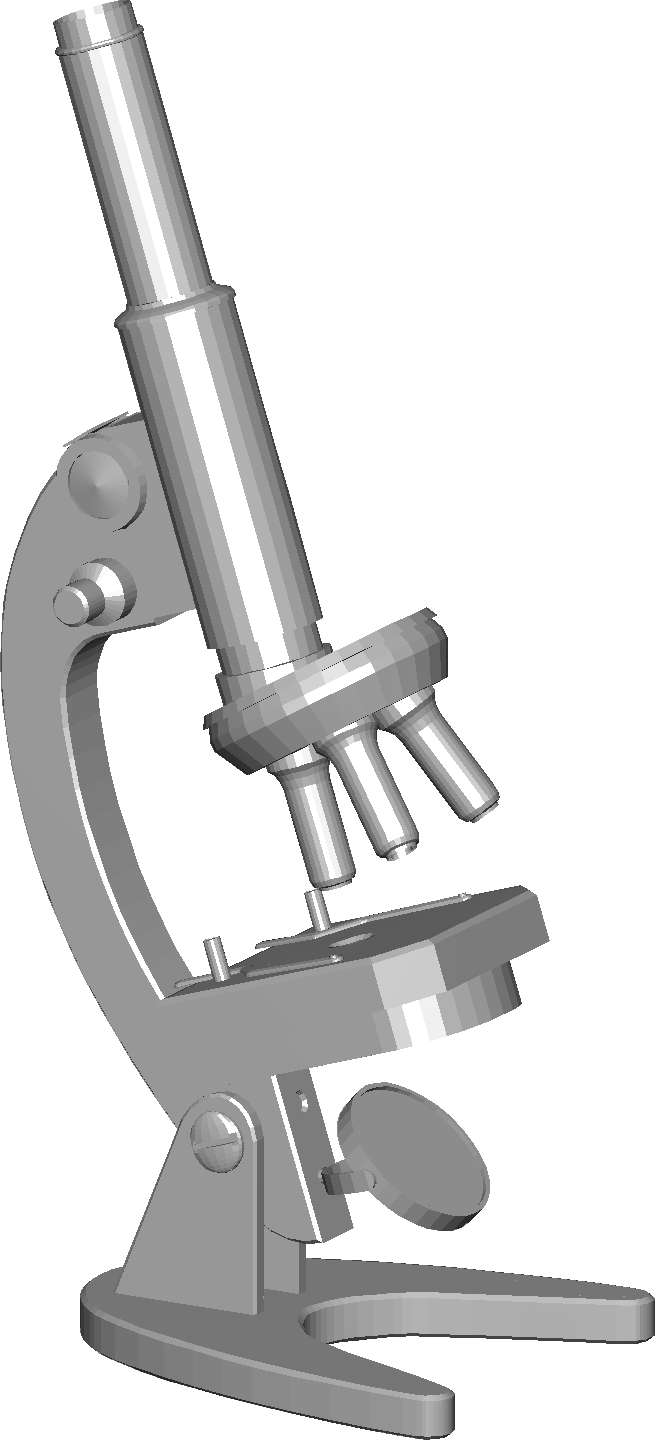
\includegraphics[width=0.5\linewidth]{./fig/eval/15microscope.png}  
		\caption{Microscope} 	
	\end{subfigure} \\ 
	\begin{subfigure}[t]{0.19\linewidth} \centering
		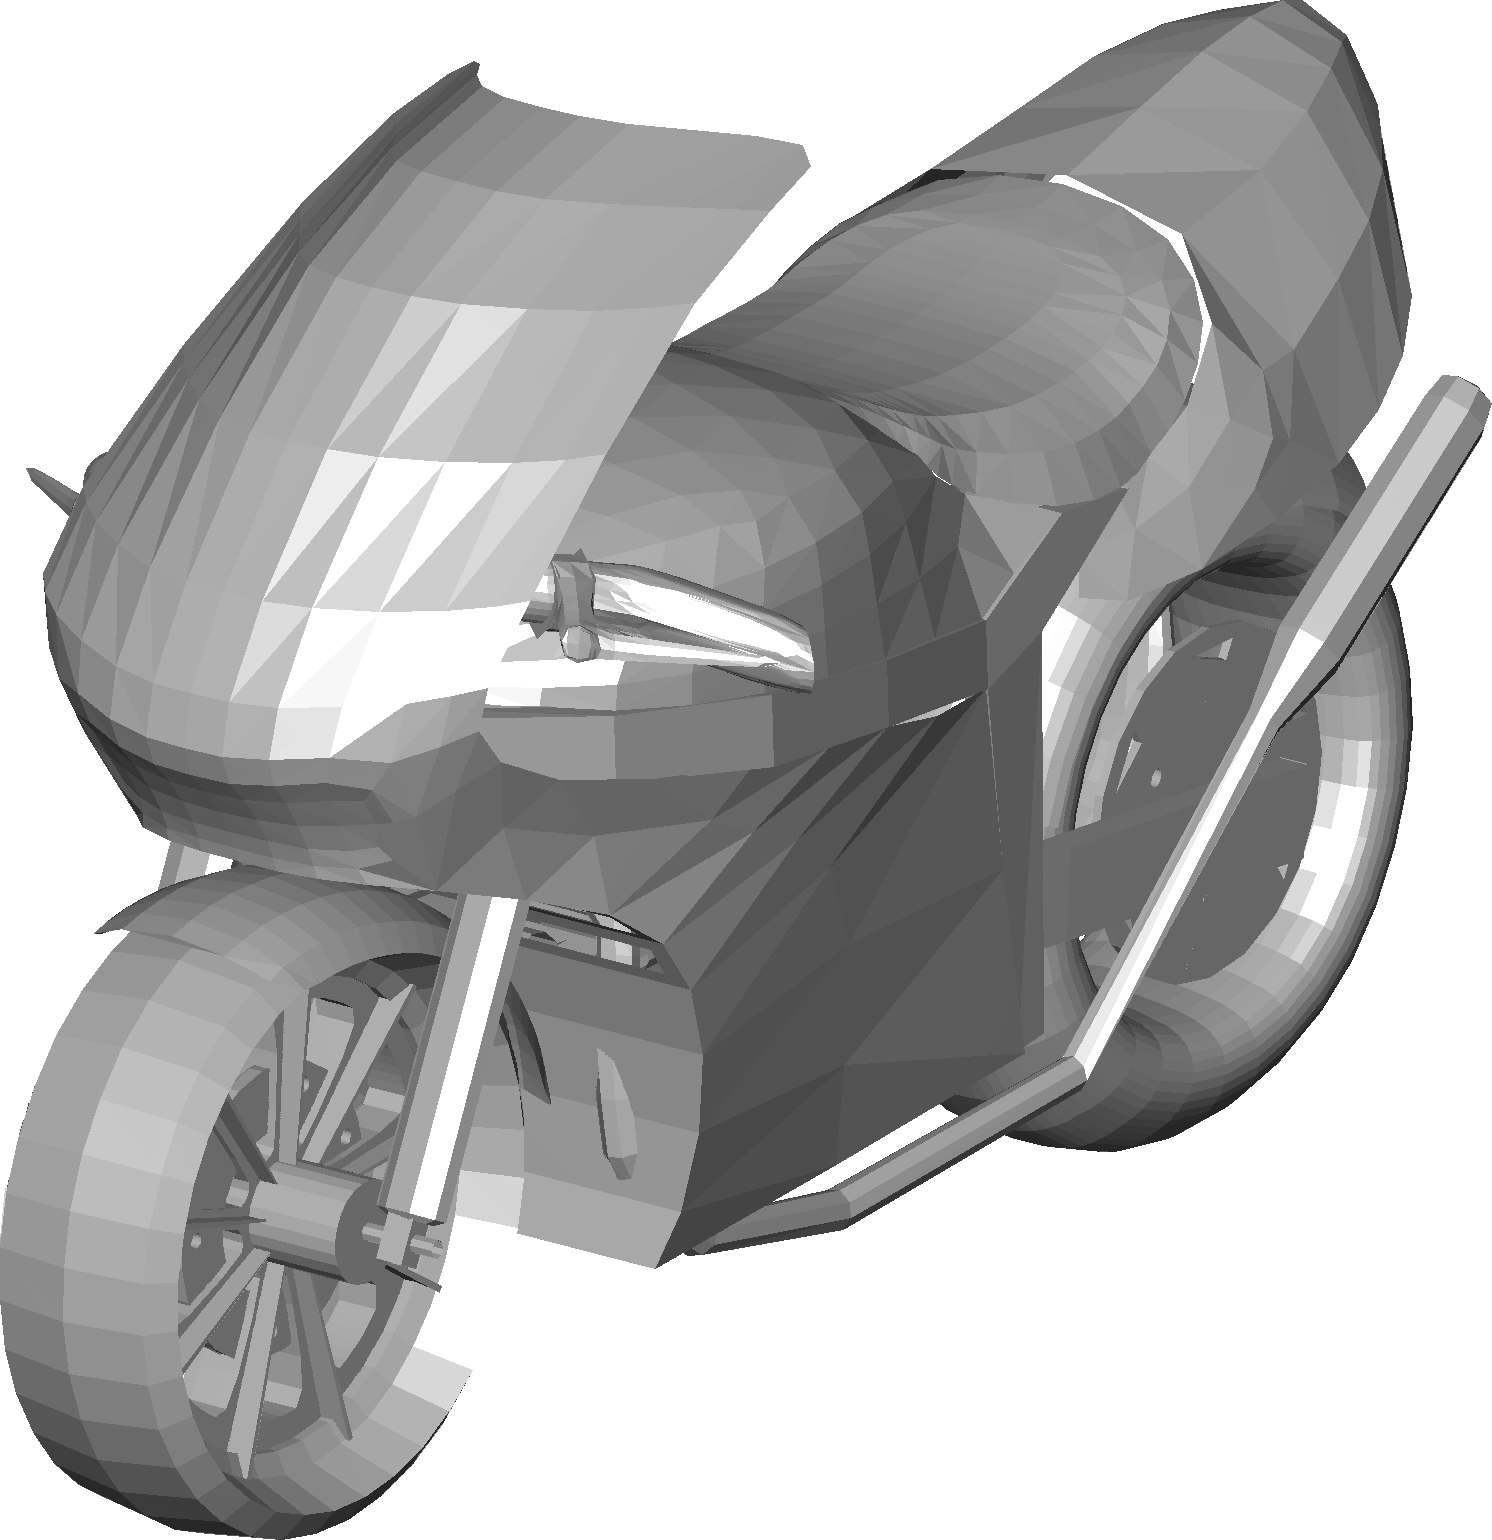
\includegraphics[width=1\linewidth]{./fig/eval/16motorbike.png}  
		\caption{Motorbike} 	
	\end{subfigure}
	\begin{subfigure}[t]{0.19\linewidth} \centering
		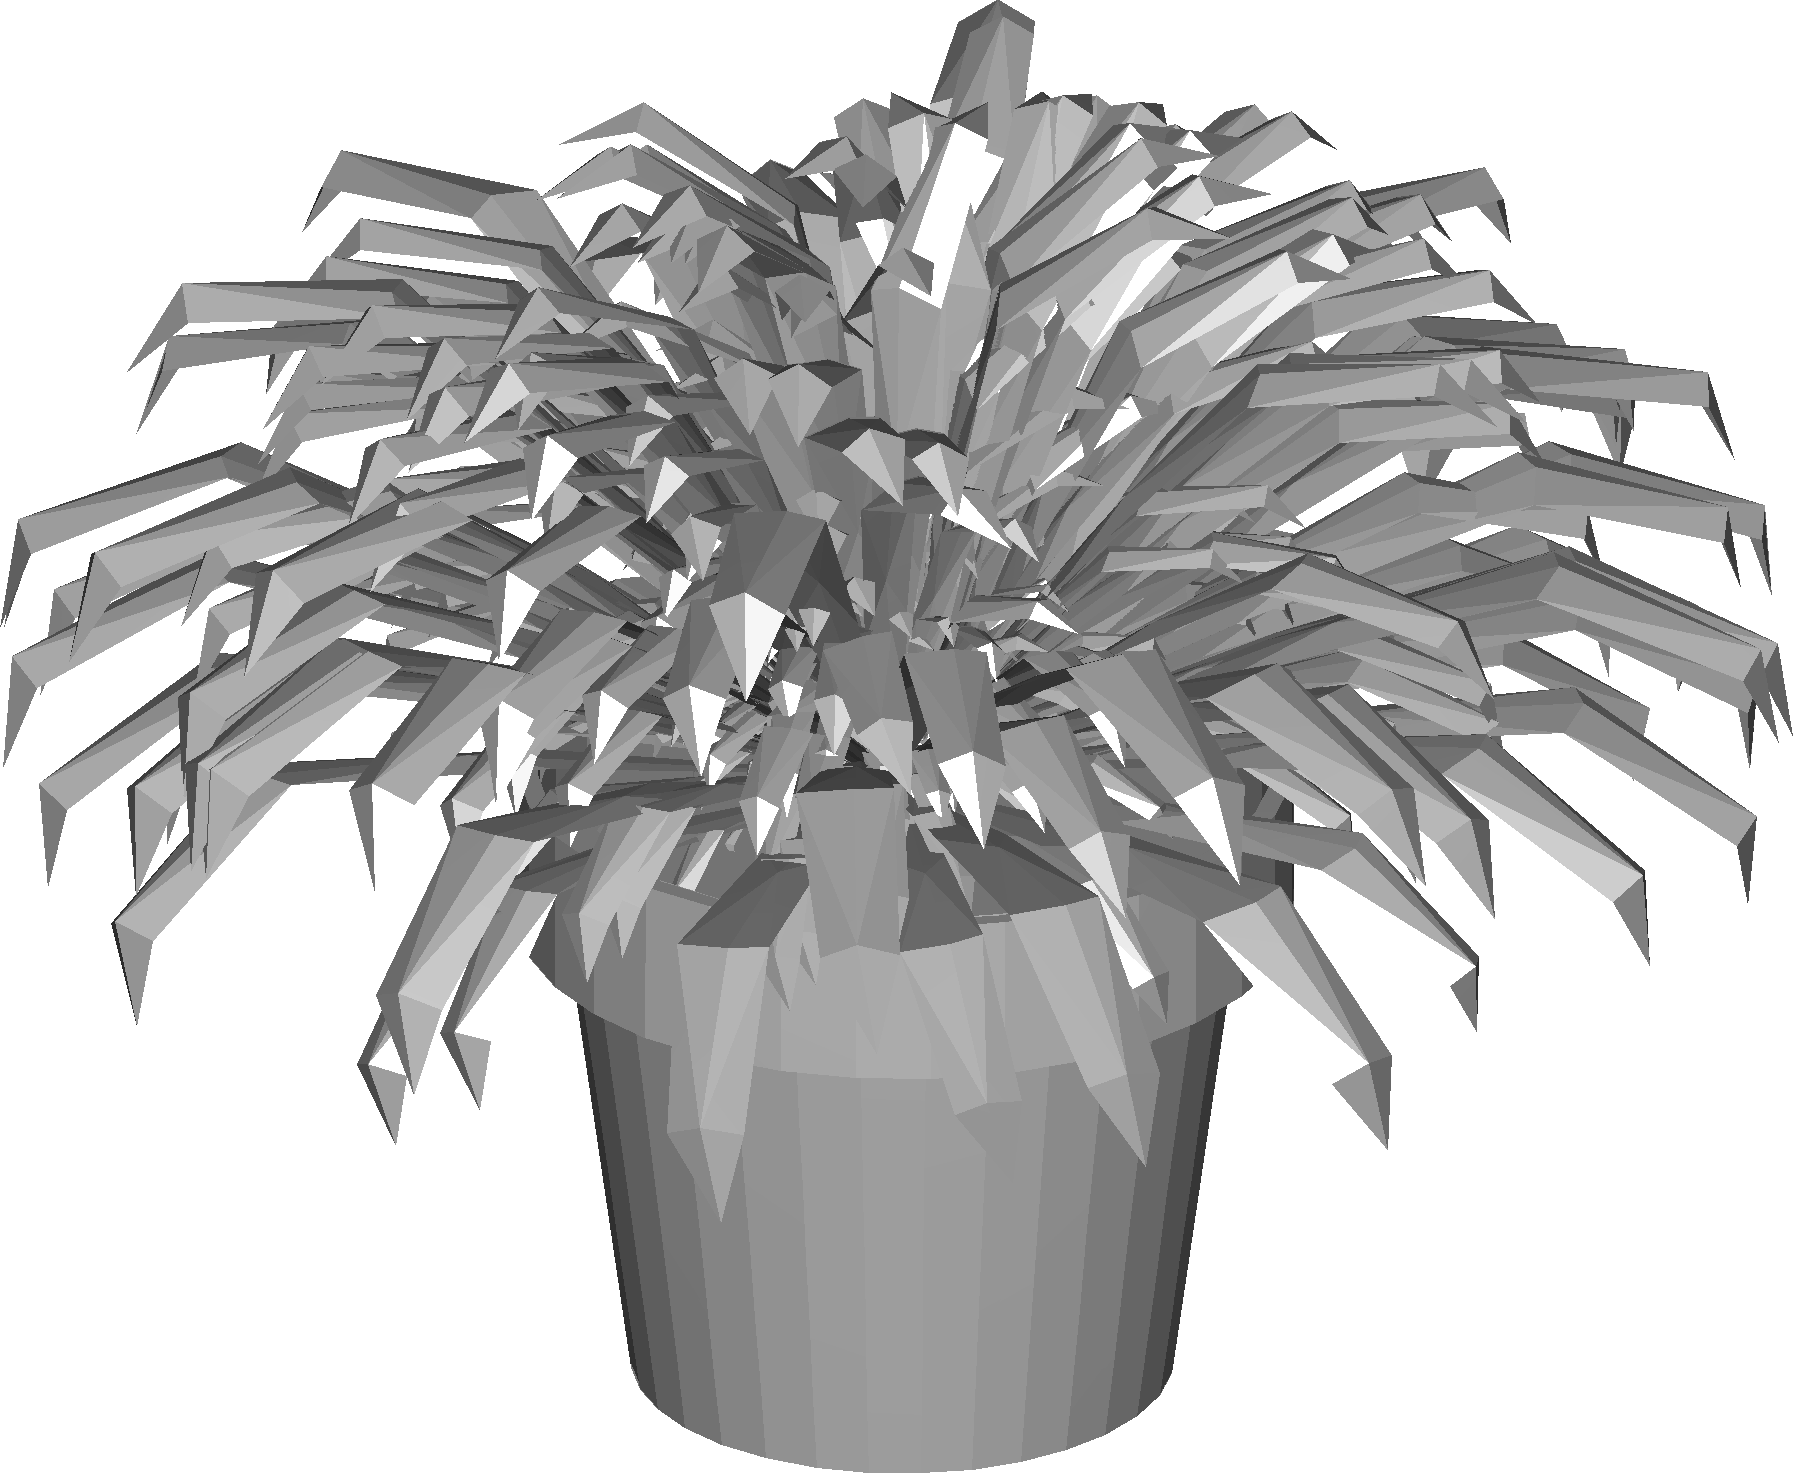
\includegraphics[width=1\linewidth]{./fig/eval/17plant.png}  
		\caption{Plant} 	
	\end{subfigure}
	\begin{subfigure}[t]{0.19\linewidth} \centering
		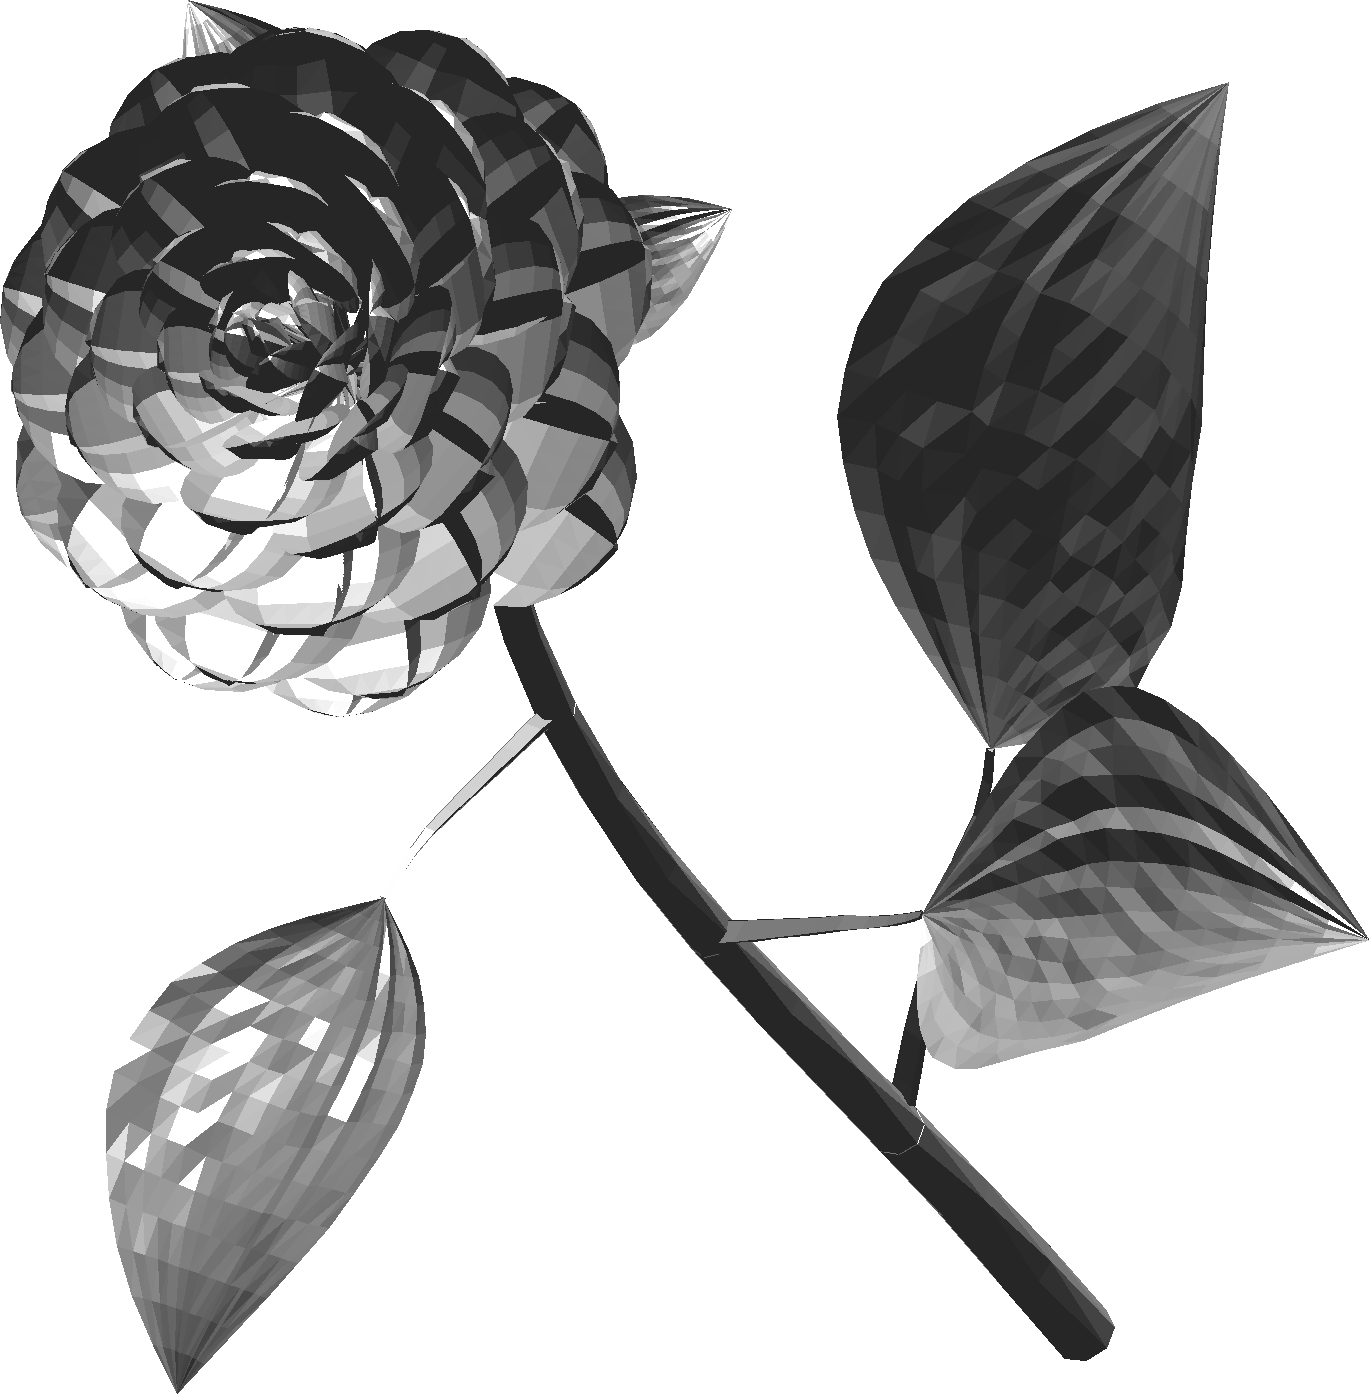
\includegraphics[width=1\linewidth]{./fig/eval/18rose.png}  
		\caption{Rose} 	
	\end{subfigure}
	\begin{subfigure}[t]{0.19\linewidth} \centering
		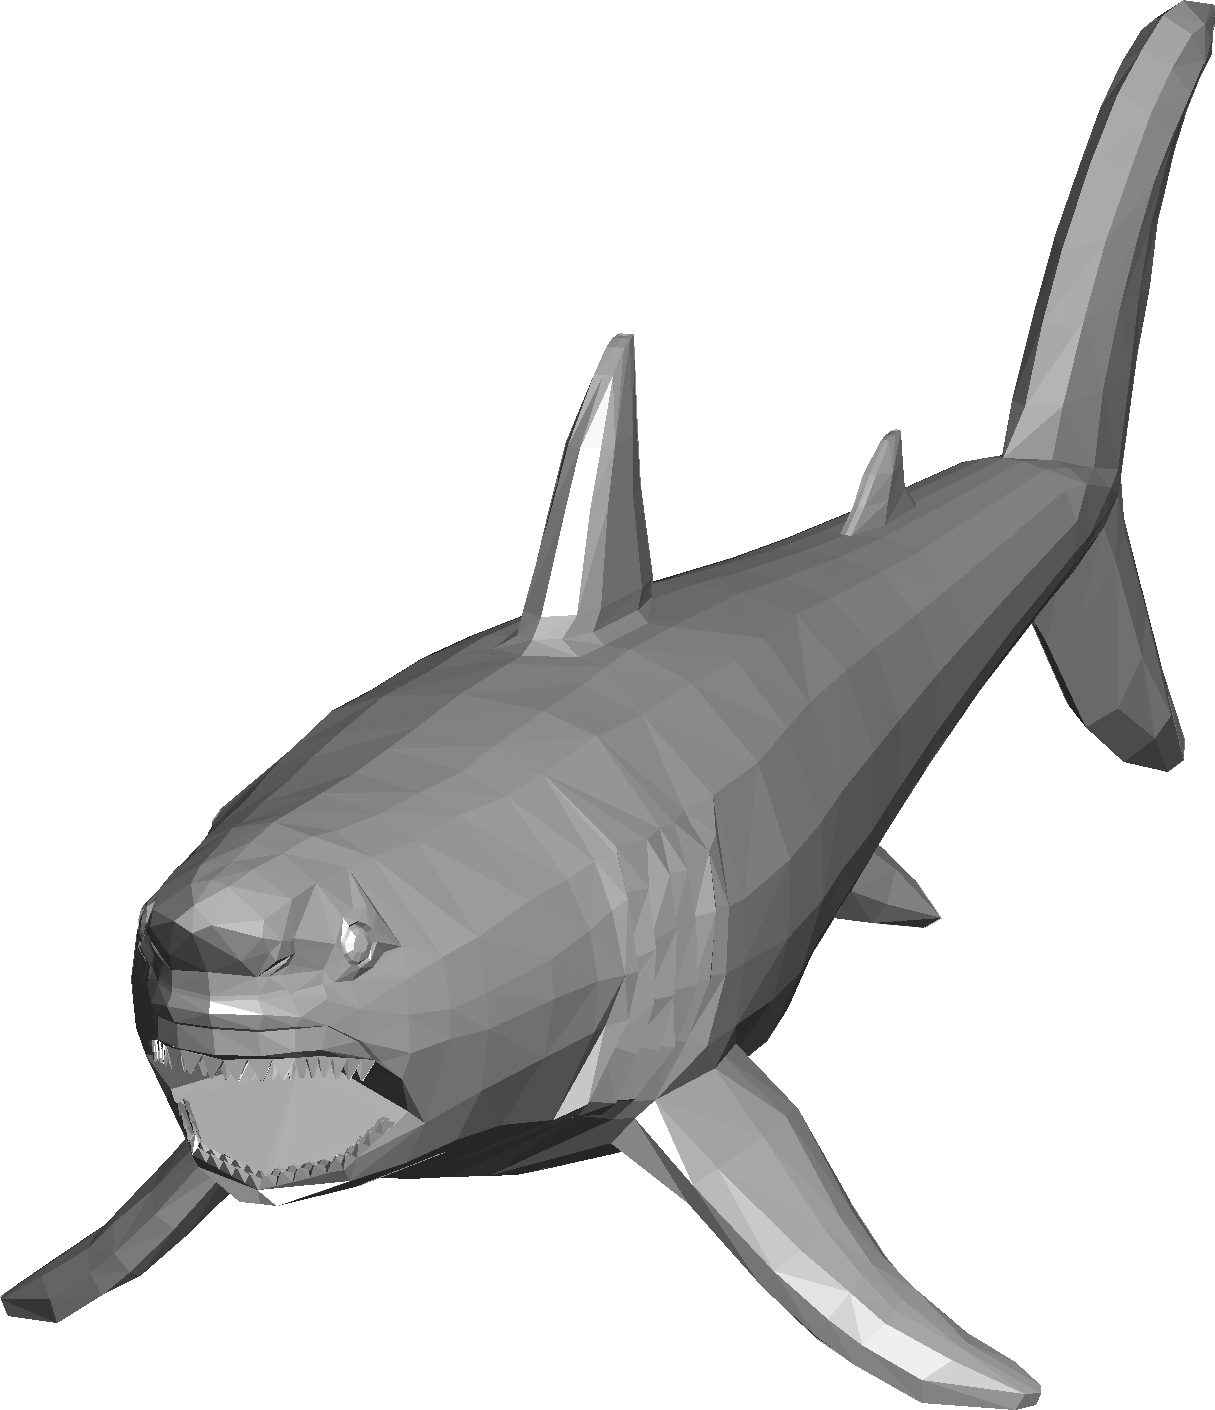
\includegraphics[width=1\linewidth]{./fig/eval/19shark.png}  
		\caption{Shark} 	
	\end{subfigure} 
	\begin{subfigure}[t]{0.19\linewidth} \centering
		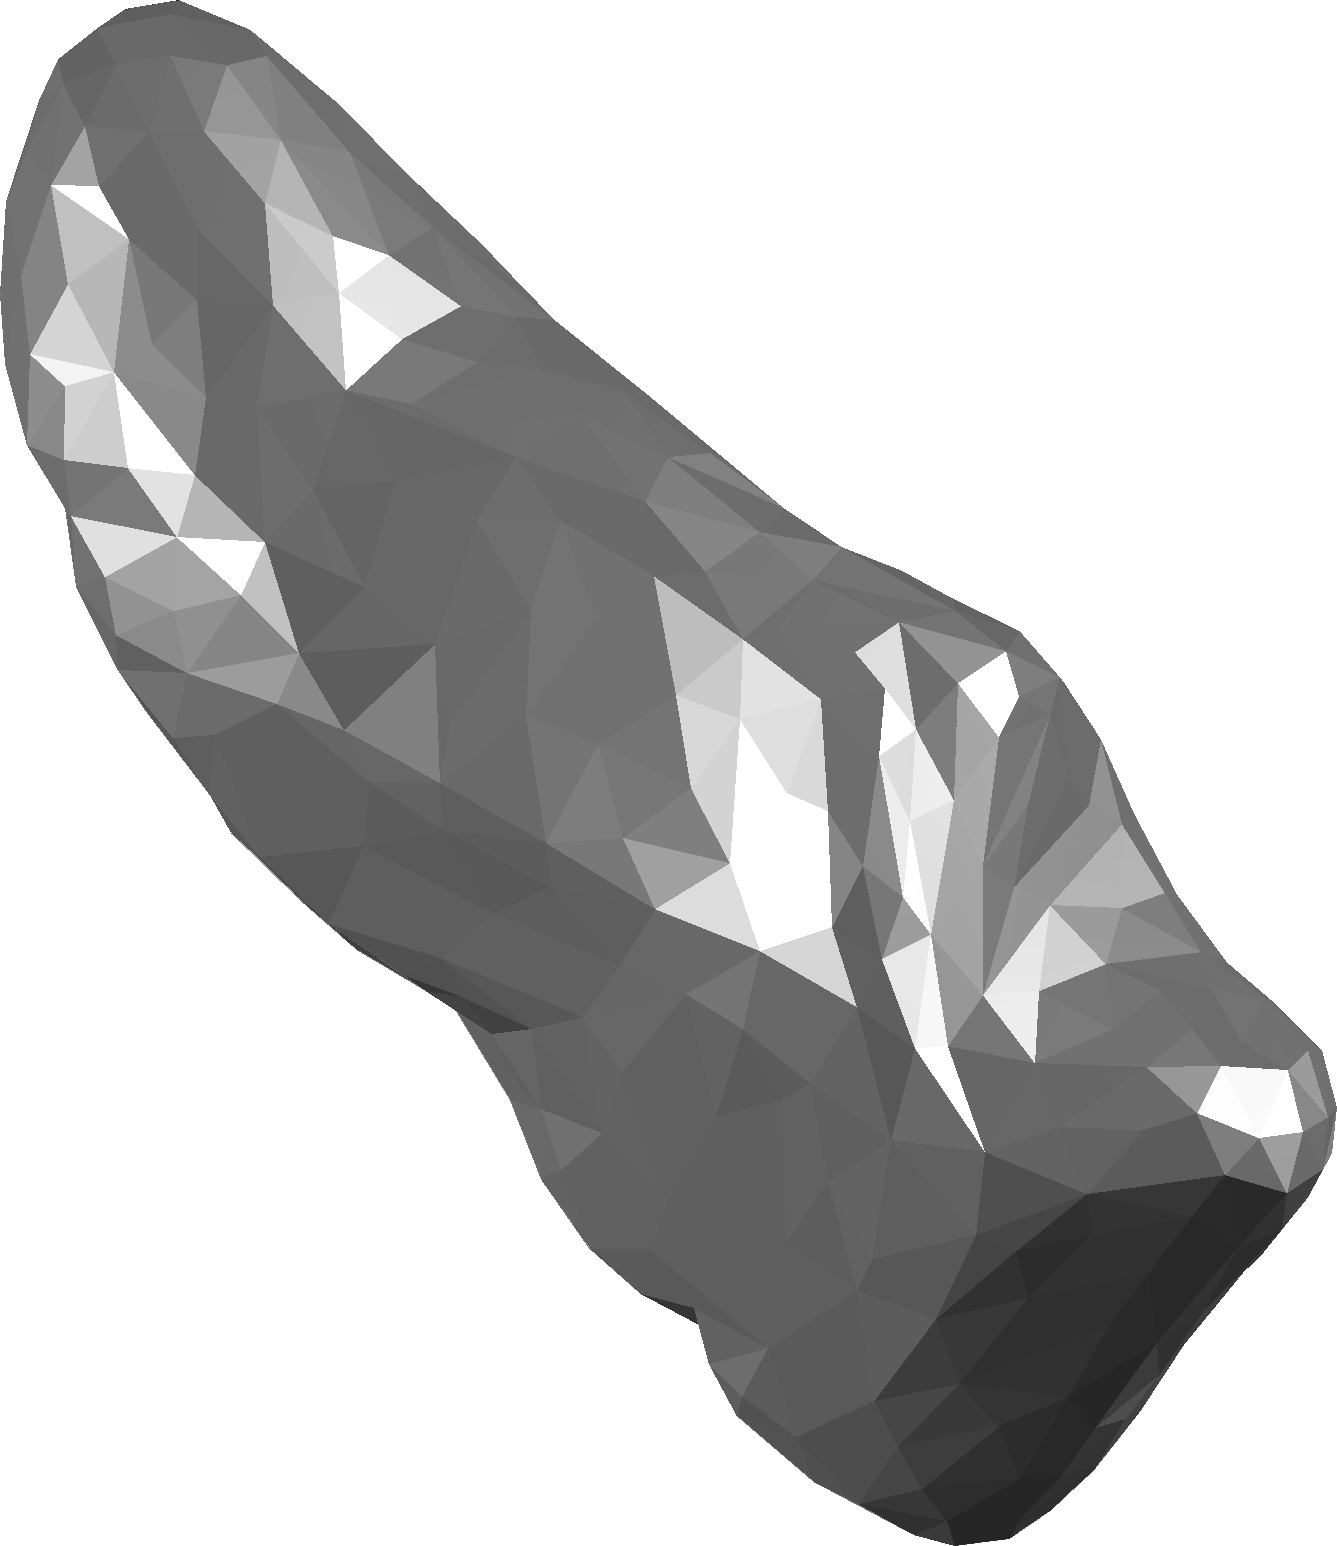
\includegraphics[width=1\linewidth]{./fig/eval/20shoe.png}  
		\caption{Shoe} 	
	\end{subfigure} \\ 
	\begin{subfigure}[t]{0.19\linewidth} \centering
		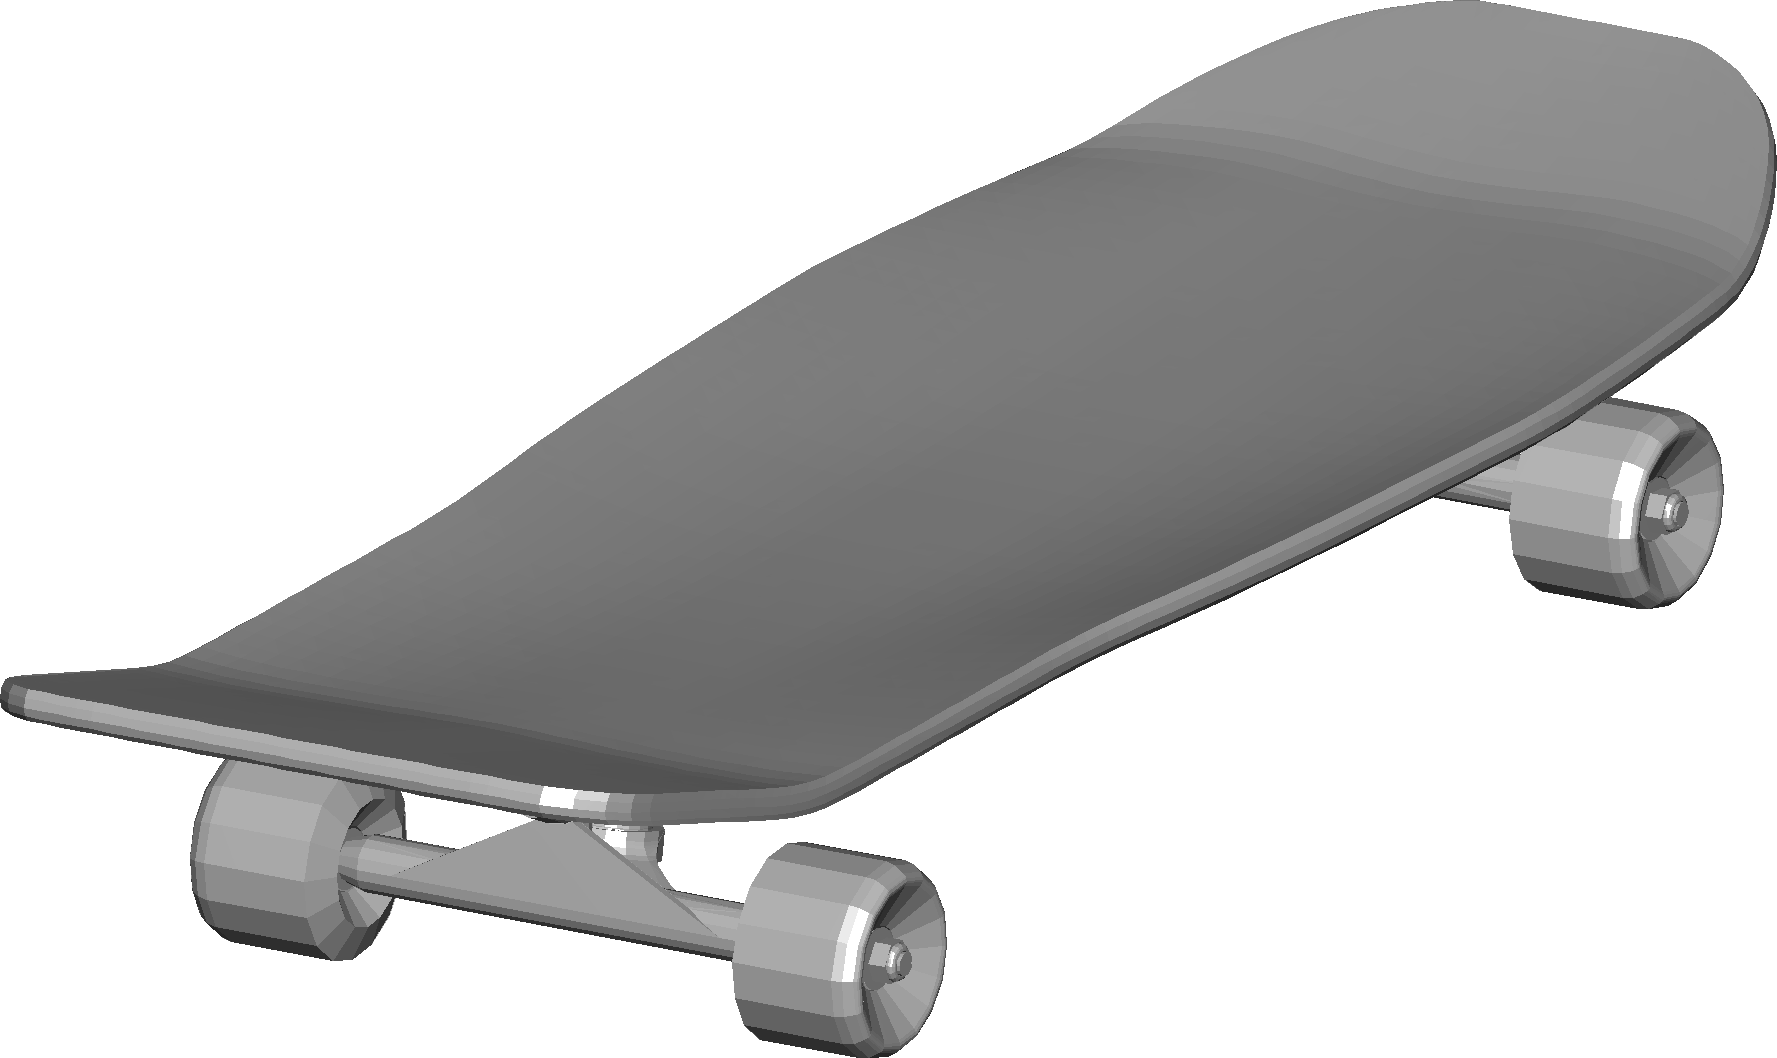
\includegraphics[width=1\linewidth]{./fig/eval/21skateboard.png}  
		\caption{Skateboard} 	
	\end{subfigure}
	\begin{subfigure}[t]{0.19\linewidth} \centering
		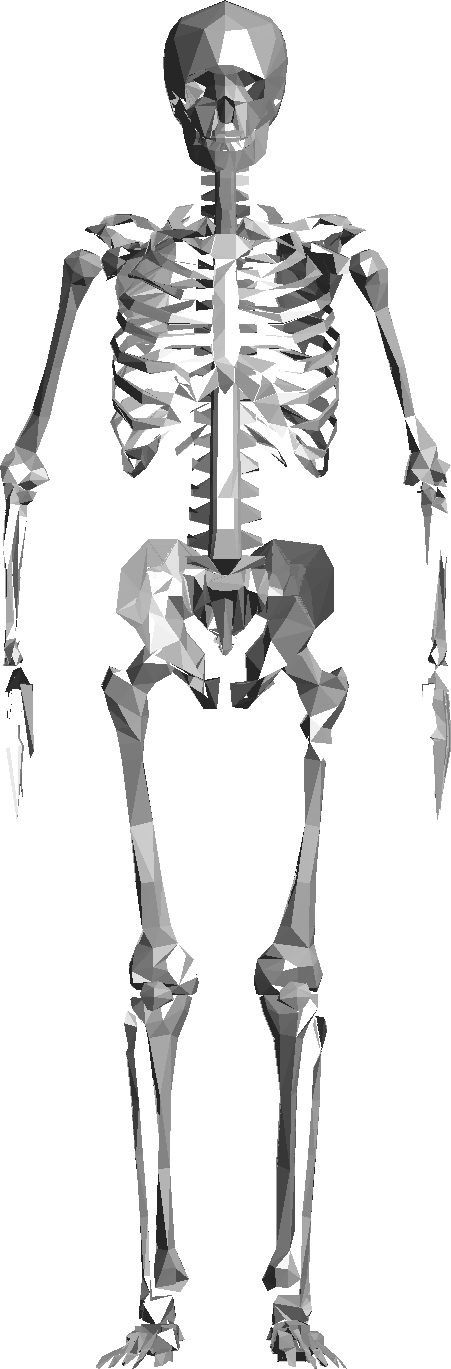
\includegraphics[width=0.3\linewidth]{./fig/eval/22skeleton.png}  
		\caption{Skeleton} 	
	\end{subfigure}
	\begin{subfigure}[t]{0.19\linewidth} \centering
		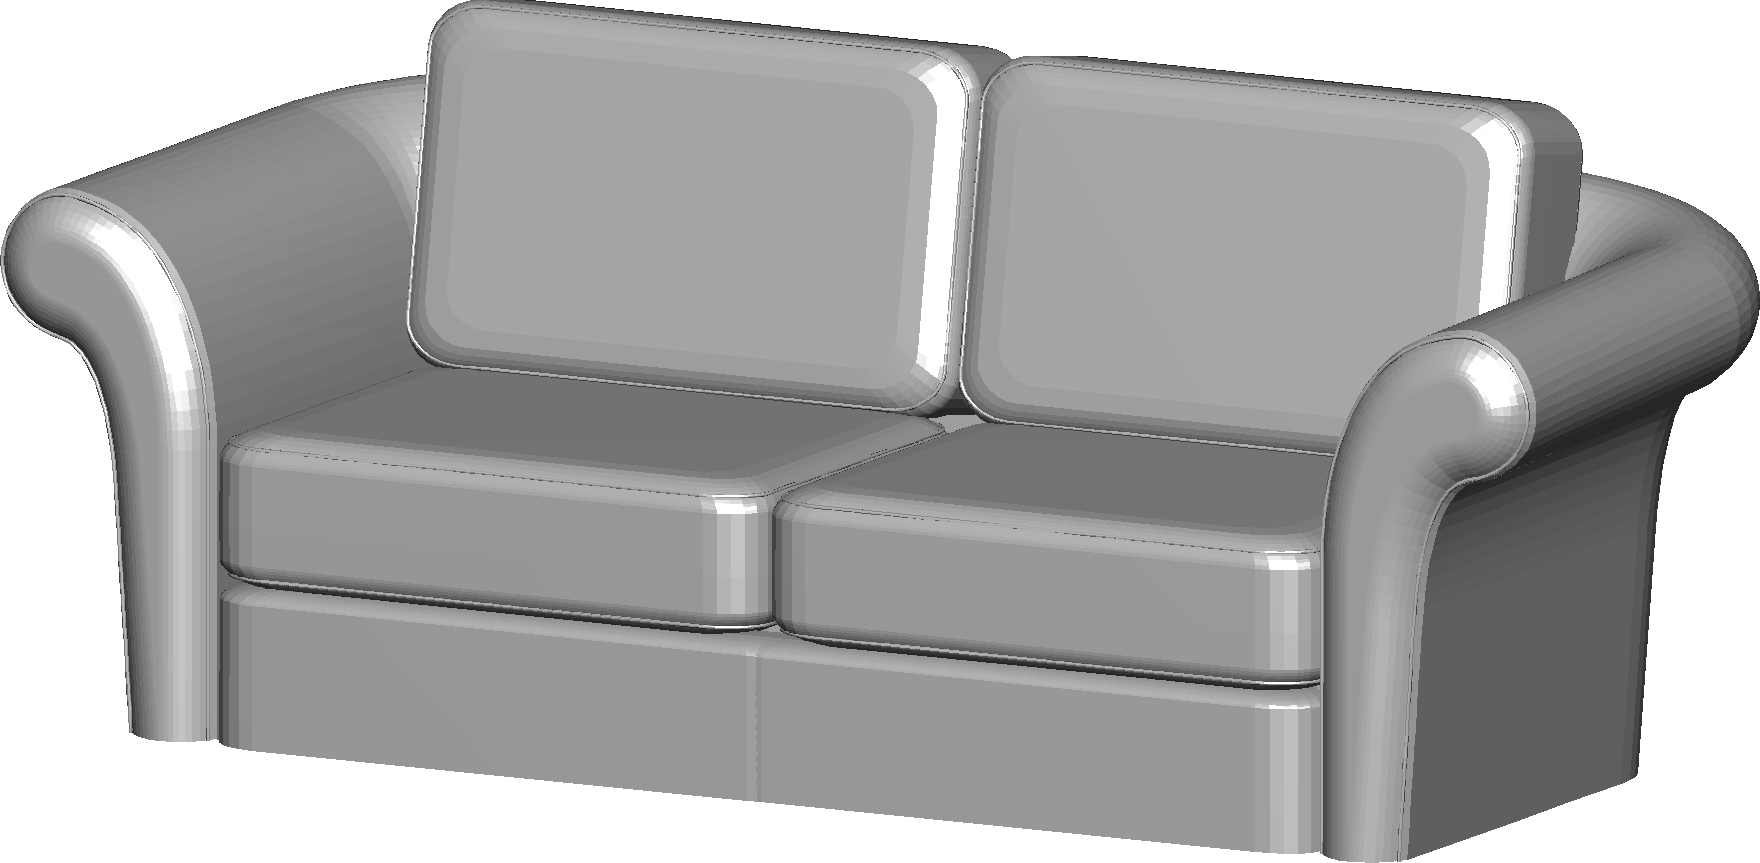
\includegraphics[width=1\linewidth]{./fig/eval/23sofa.png}  
		\caption{Sofa} 	
	\end{subfigure}
	\begin{subfigure}[t]{0.19\linewidth} \centering
		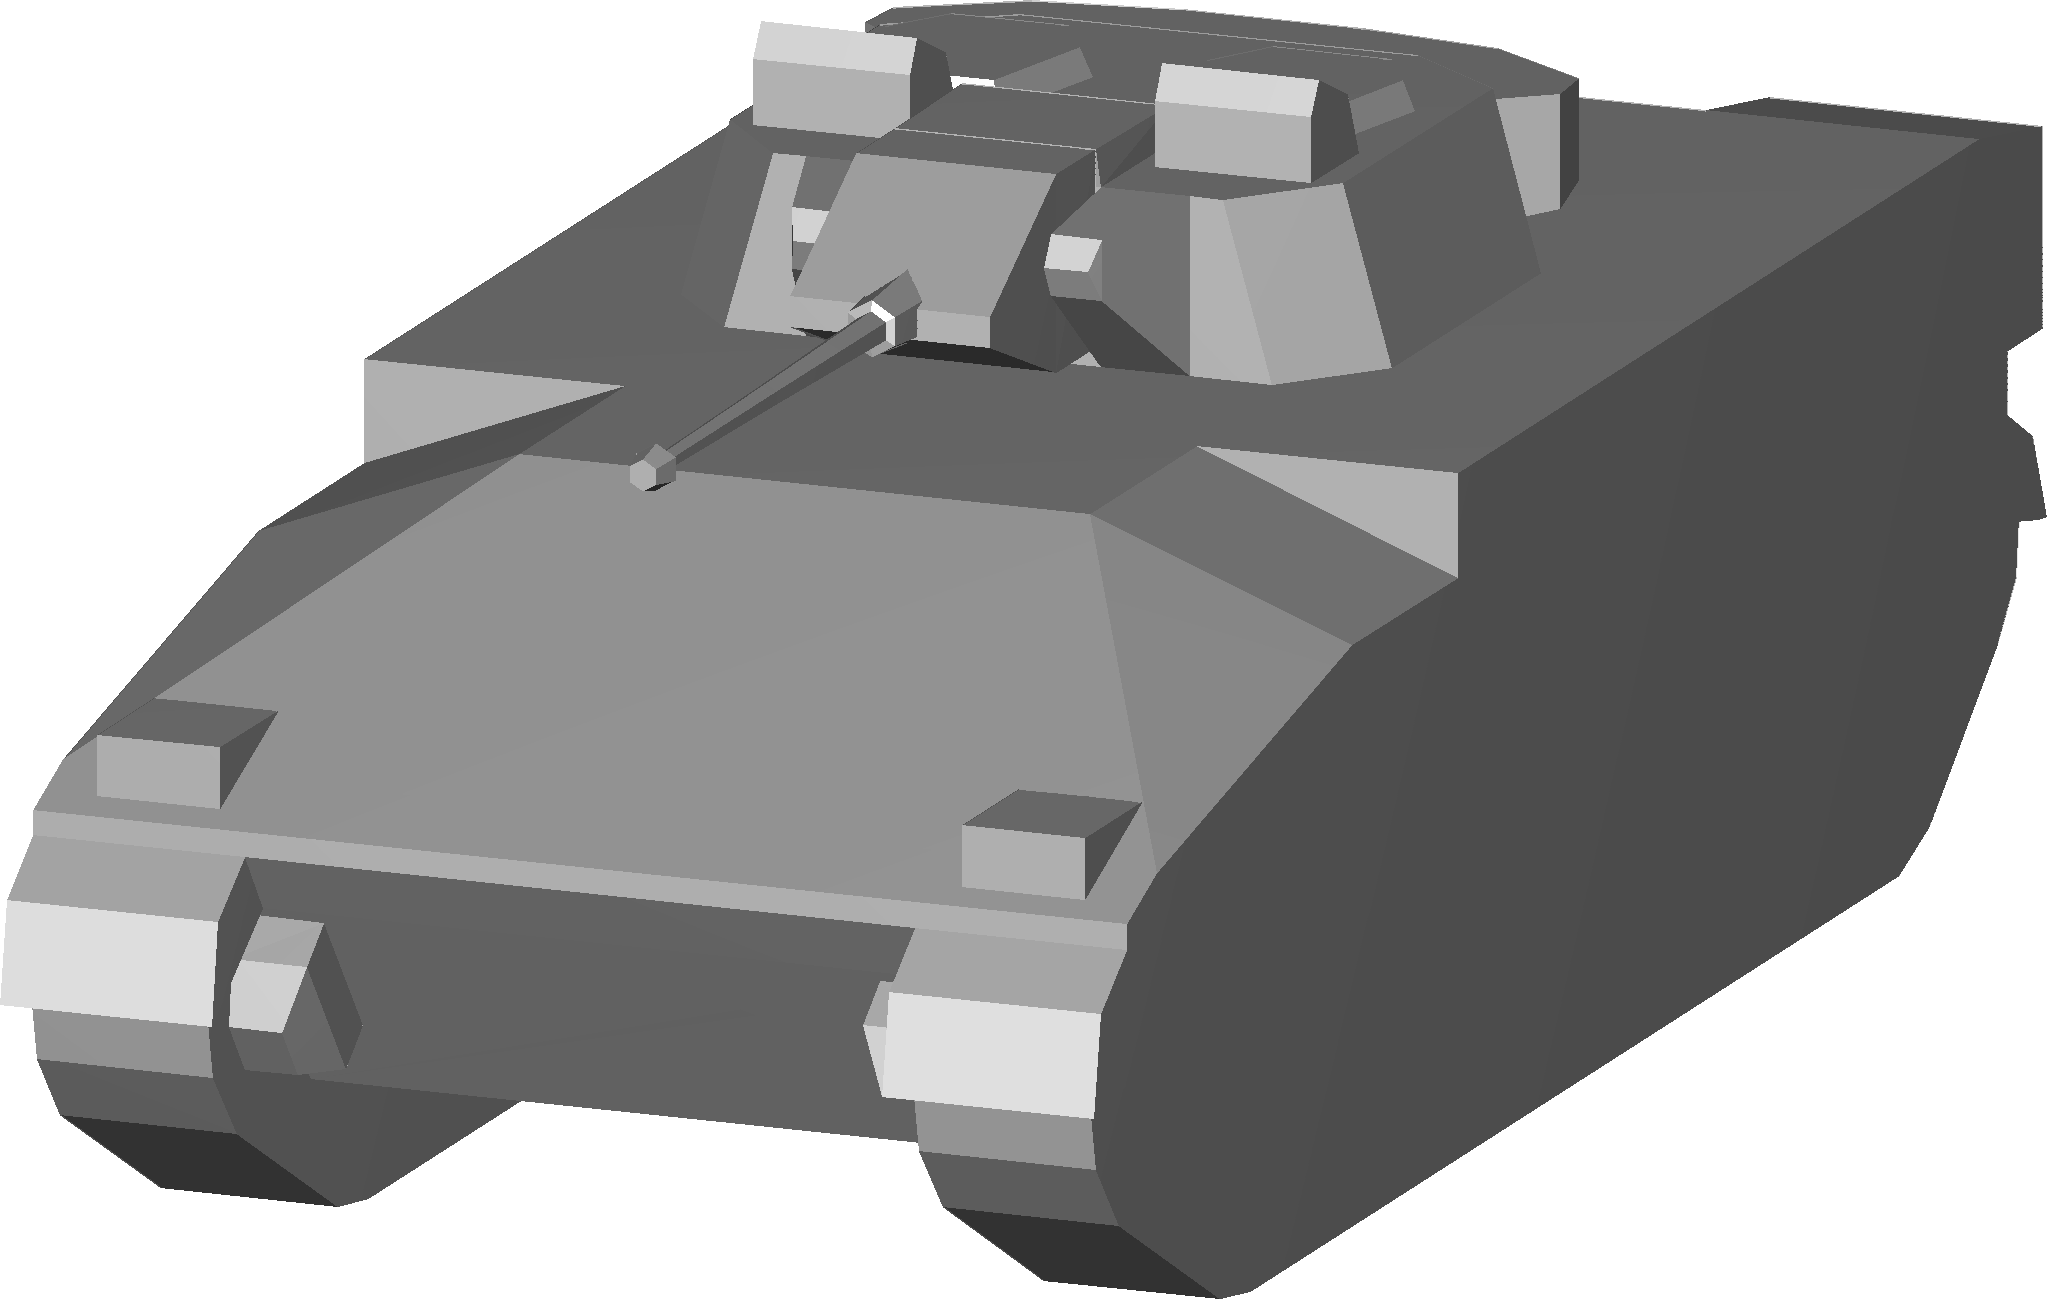
\includegraphics[width=1\linewidth]{./fig/eval/24tank.png}  
		\caption{Tank} 	
	\end{subfigure} 
	\begin{subfigure}[t]{0.19\linewidth} \centering
		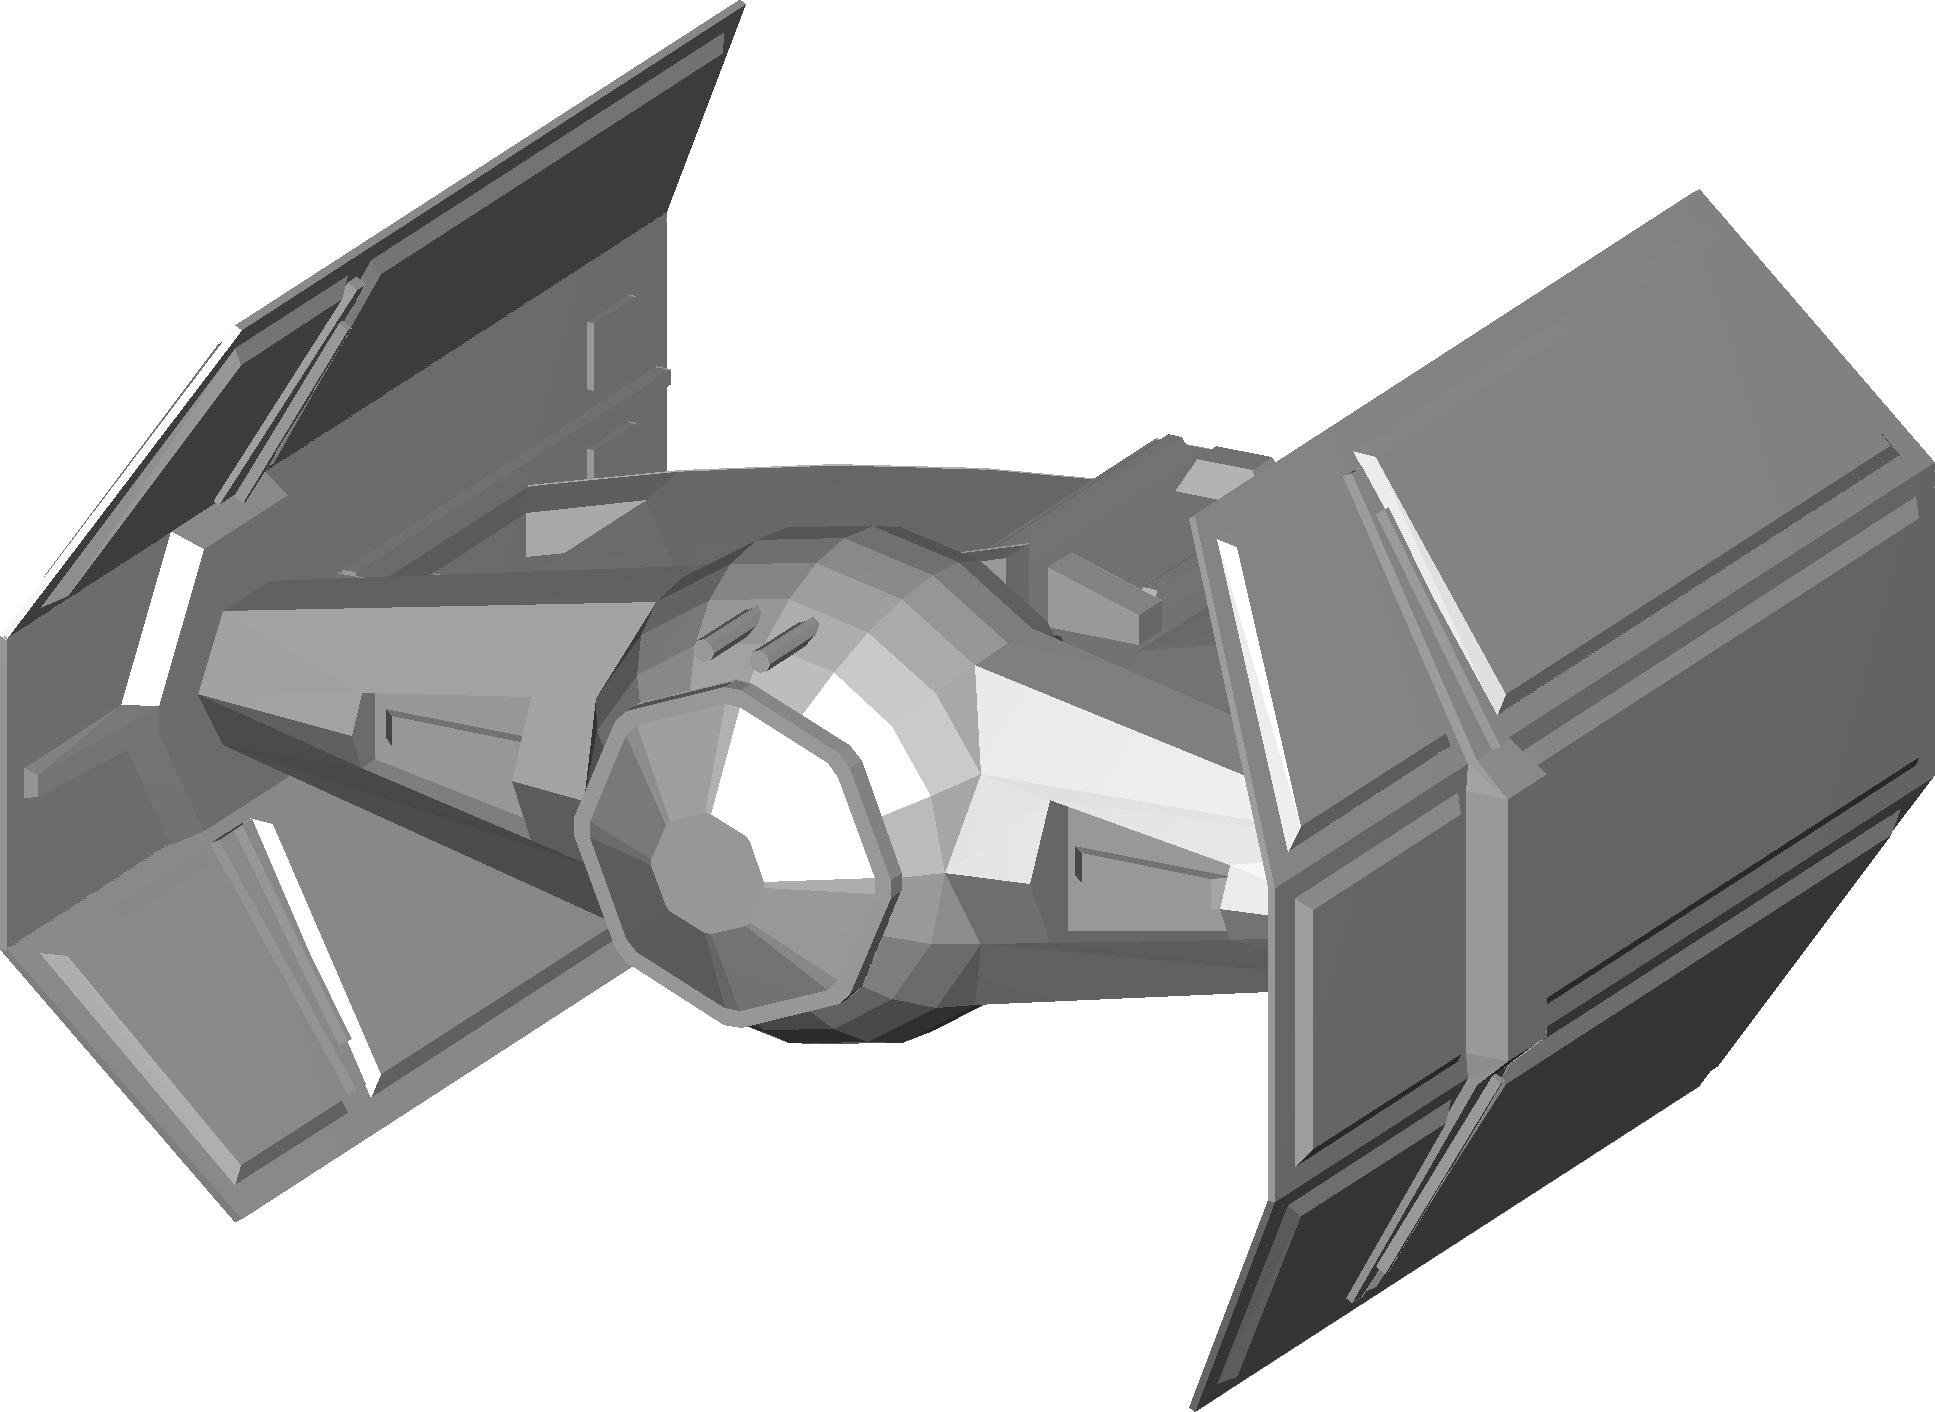
\includegraphics[width=1\linewidth]{./fig/eval/25tiefighter.png}  
		\caption{Tiefighter} 	
	\end{subfigure} 
	\caption{The sample 3D shapes in the \meshset dataset.}
	\label{fig/eval/sampleshapes}
\end{figure}


\subsection{Experimental setup}
\label{sec/eval/variation}
% done 
In the evaluation experiments, a series of transformed shapes were created from the reference shape with different magnitudes of a test parameter. Repeatability scores were computed by matching the two sets of interest points to each other, according to equation \ref{eqn/eval/rptarea}. The overall performance of one dataset was measured by averaging the $\areascore$ scores across all shapes in the evaluation dataset. 

% done 
The characteristics of the interest point detectors were evaluated under five different variations. These include (1) rotation, (2) translation, (3) scale, (4) sampling density and (5) sampling noise. 
For the \mriset and the \stereoset datasets, such variations were introduced during the process of shape acquisition. Shapes in the \meshset dataset were generated synthetically with different variations.

% done 
The variations applied to the evaluation datasets are described in table \ref{tab/eval/datavar}. Although image compression rate and lighting change were also evaluated for image-based detectors \cite{Mikolajczyk2005}, similar variations are not necessary for 3D shape data because they are unaffected by such factors. 

% done 
\begin{table}[ht]
\centering
\begin{tabular}{|cc|ccccc|}
\hline
\multirow{2}{*}{ } & \multirow{2}{*}{ } & \multicolumn{5}{c}{\textbf{Variations}} \\ \cline{3-7} 
& & \textbf{Noise} & \textbf{Density} & \textbf{Scale} & \textbf{Rotation} & \textbf{Translation} \\
\hline
\multirow{3}{*}{\textbf{Dataset}} & \meshset & \checkmark & \checkmark & \checkmark & \checkmark & \\
& \mriset & \checkmark & & & \checkmark & \checkmark \\
& \stereoset & \checkmark & \checkmark & \checkmark & \checkmark & \checkmark \\
\hline
\end{tabular}
\caption{\textbf{Properties of the evaluation datasets.}}
\label{tab/eval/datavar}
\end{table}

Performances of the candidate detectors were measured as each test parameter was varied individually, keeping all the other parameters at their default values. Sampling-related parameters (\ie noise level and sampling density) were applied to all shape instances, whilst pose parameters (\ie rotation, translation and scale) were applied to only one instance in each matching pair. Some parameters were defined in terms of $L$, which was the largest dimension of the voxelised reference shapes. In this experiment, the maximum value of $L$ was limited to $200$ by the voxelisation process. The default parameters for the reference shapes, and the number of transformed shapes created for matching, are summarised in table \ref{tab/eval/referenceparam}. 

\begin{table}[ht]
\centering
\begin{tabular}{|c|c|}
\hline
\multicolumn{2}{c}{ \textbf{Default parameters for reference shapes }} \\ 
\hline 
\textbf{Parameter} & \textbf{Value} \\
\hline
Default point cloud size & $50000$ points\\
Default noise $\sigma_{n}$ & $0.0025L$\\ 
Default rotation & $0^{\circ}$\\
Maximum $L$ & $200$ voxels\\
Default $\sigma_{\textrm{KDE}}$ in $g(\cdot,\sigma_{\textrm{KDE}})$ & $1.5$ voxels \\ 
Distance threshold $\disp$ & $0.03L$ \\
Parameter $f$ in equation (\ref{eqn/eval/loc_vec}) & $\sqrt{8}$ \\
Number of octaves in scale-space & $4$ \\
\hline
\multicolumn{2}{c}{ \textbf{ Number of transformed shapes compared }} \\
\hline 
\textbf{Parameter} & \textbf{Value} \\
\hline
Sampling noise & 13 \\
Sampling density & 17 \\
Noise & 21 \\
Scale & 21 \\
\hline
\end{tabular}
\caption{\textbf{Reference parameters.} Reference parameters used for the reference shapes and testing shapes.}
\label{tab/eval/referenceparam}
\end{table}

\subsection{Experiments on synthetic meshes}

\subsubsection{Sampling noise}

% done
\begin{figure}[ht]
	\centering
	\begin{subfigure}[t]{0.24\linewidth}\centering
		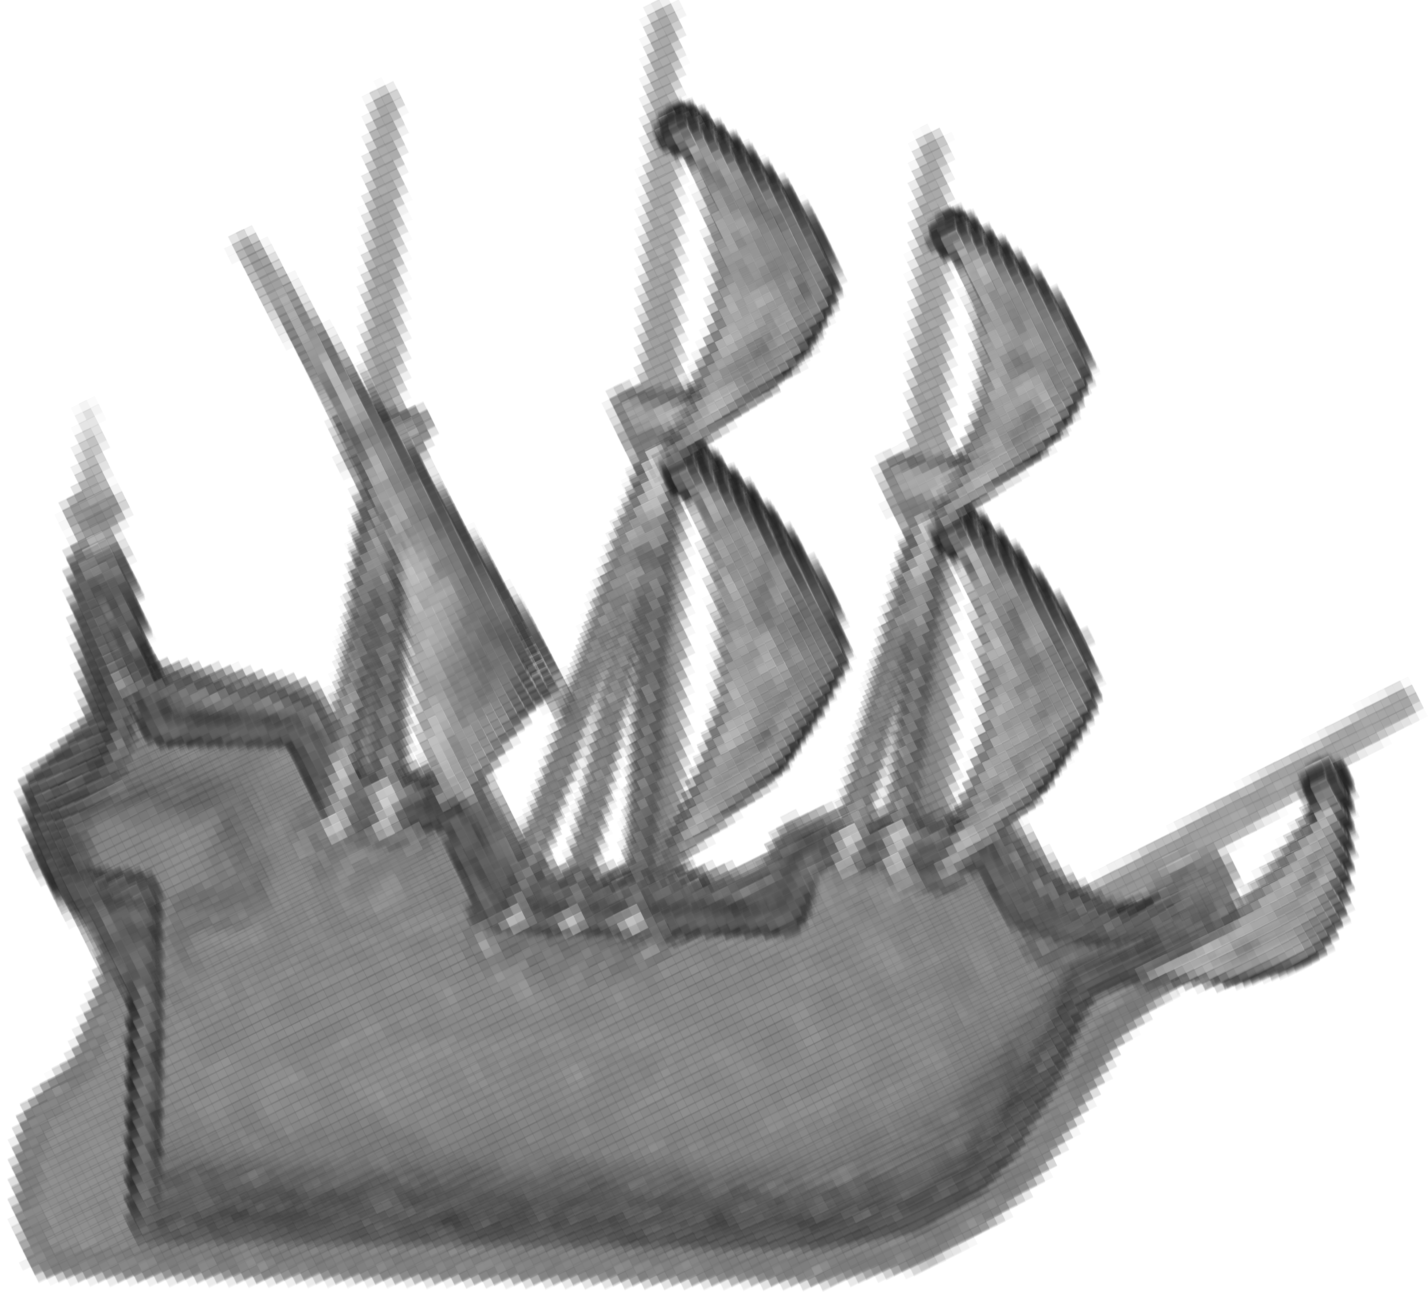
\includegraphics[width=1\linewidth]{./fig/eval/noise_none.png}
		\subcaption{$\sigma_{n} = 0$}
		\label{fig/eval/noise_none}
	\end{subfigure}
	\begin{subfigure}[t]{0.24\linewidth}\centering
		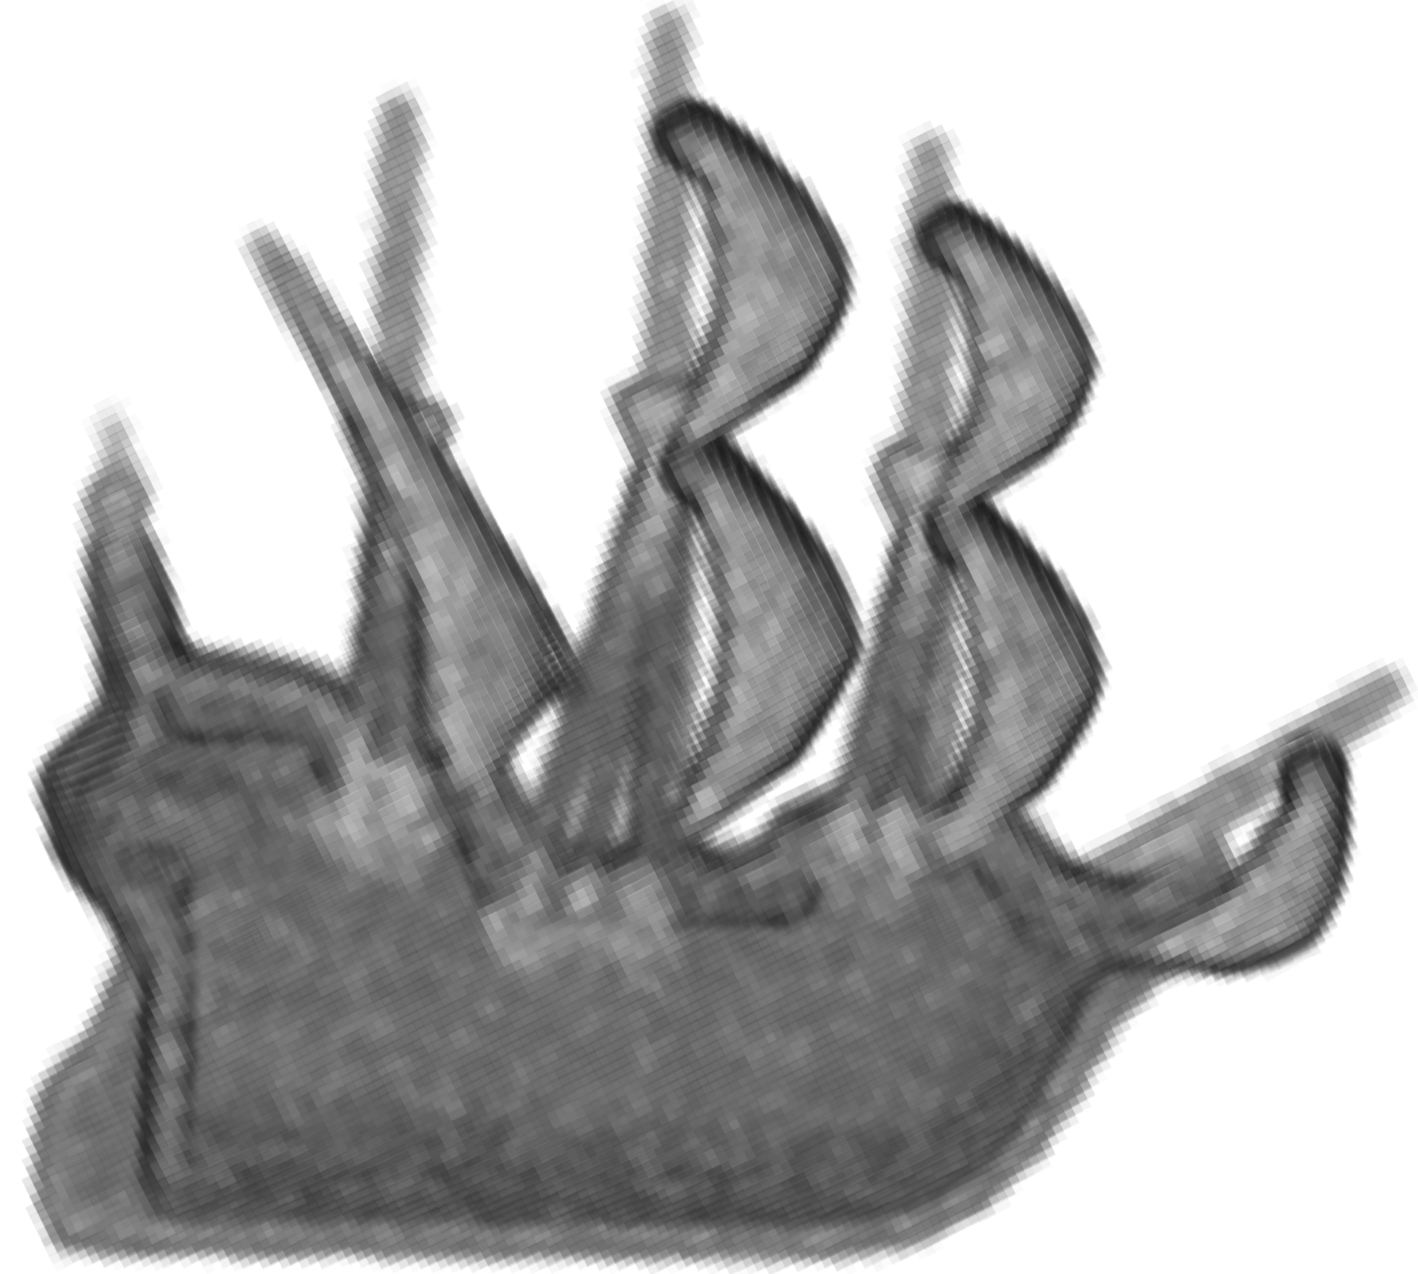
\includegraphics[width=1\linewidth]{./fig/eval/noise_low.png}
		\subcaption{$\sigma_{n} = 0.0025L$}
		\label{fig/eval/noise_low}
	\end{subfigure}
	\begin{subfigure}[t]{0.24\linewidth}\centering
		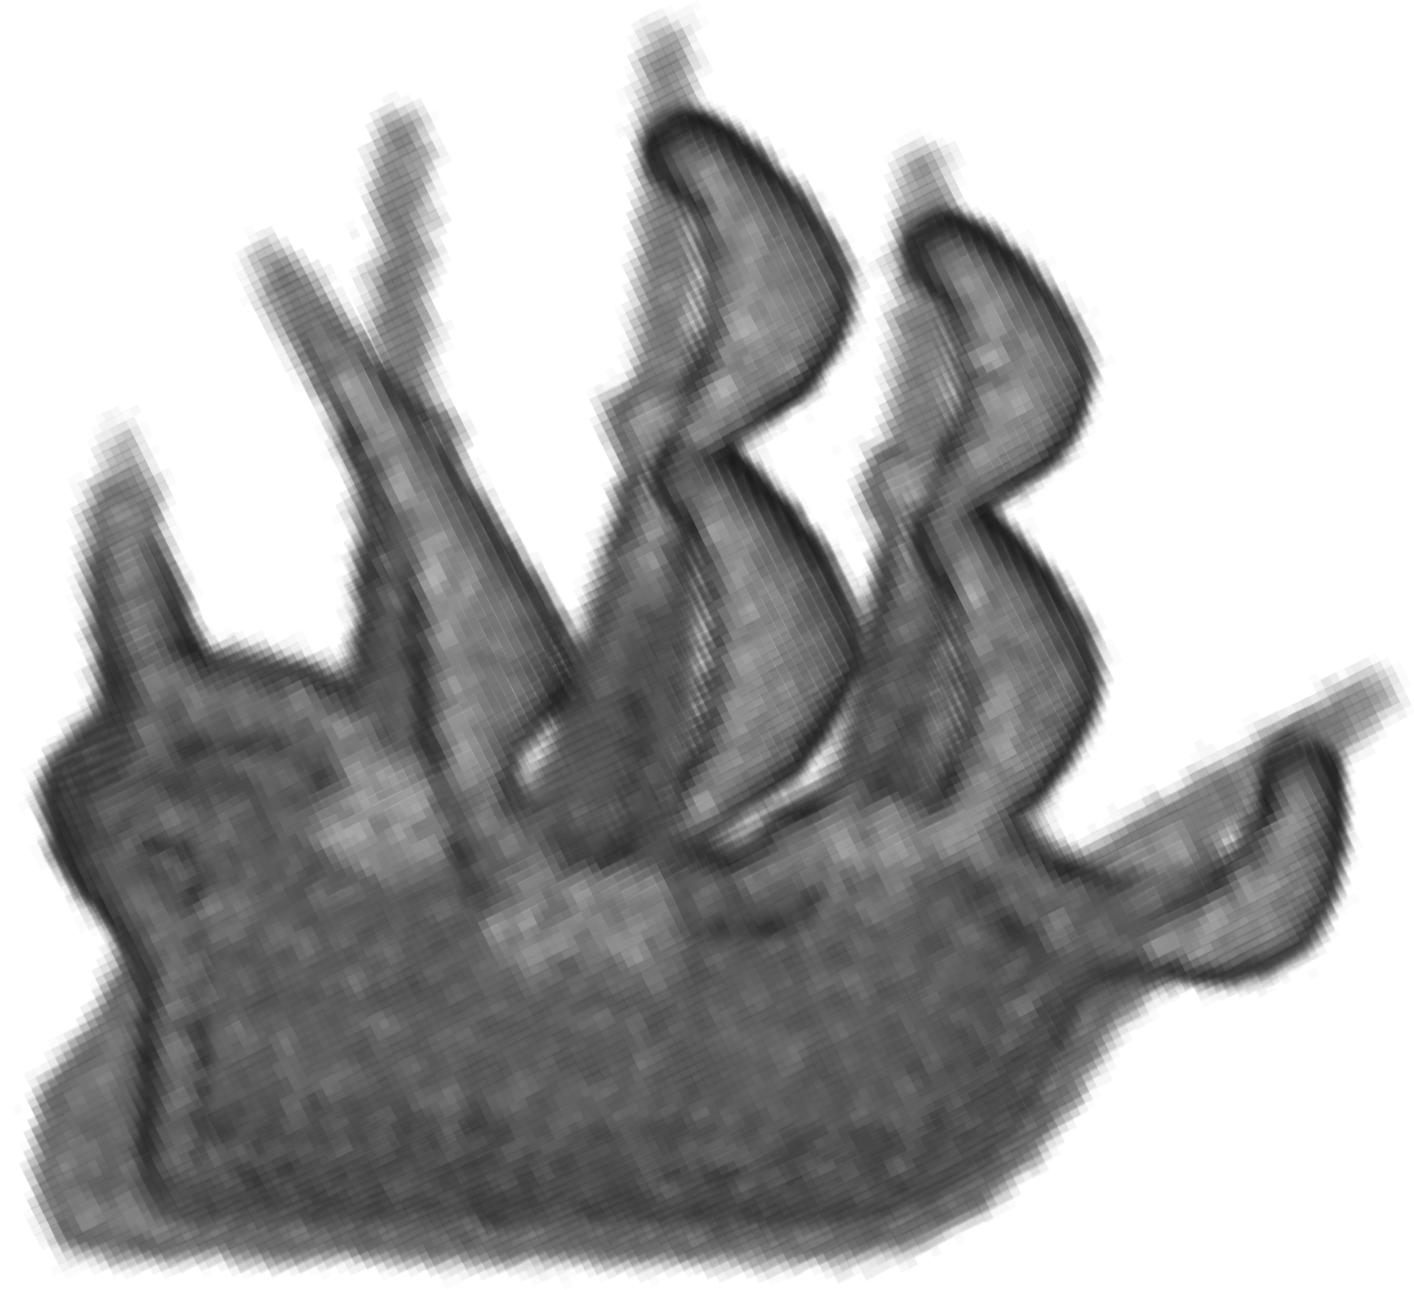
\includegraphics[width=1\linewidth]{./fig/eval/noise_mid.png}
		\subcaption{$\sigma_{n} = 0.01L$}
		\label{fig/eval/noise_mid}
	\end{subfigure}
	\begin{subfigure}[t]{0.24\linewidth}\centering
		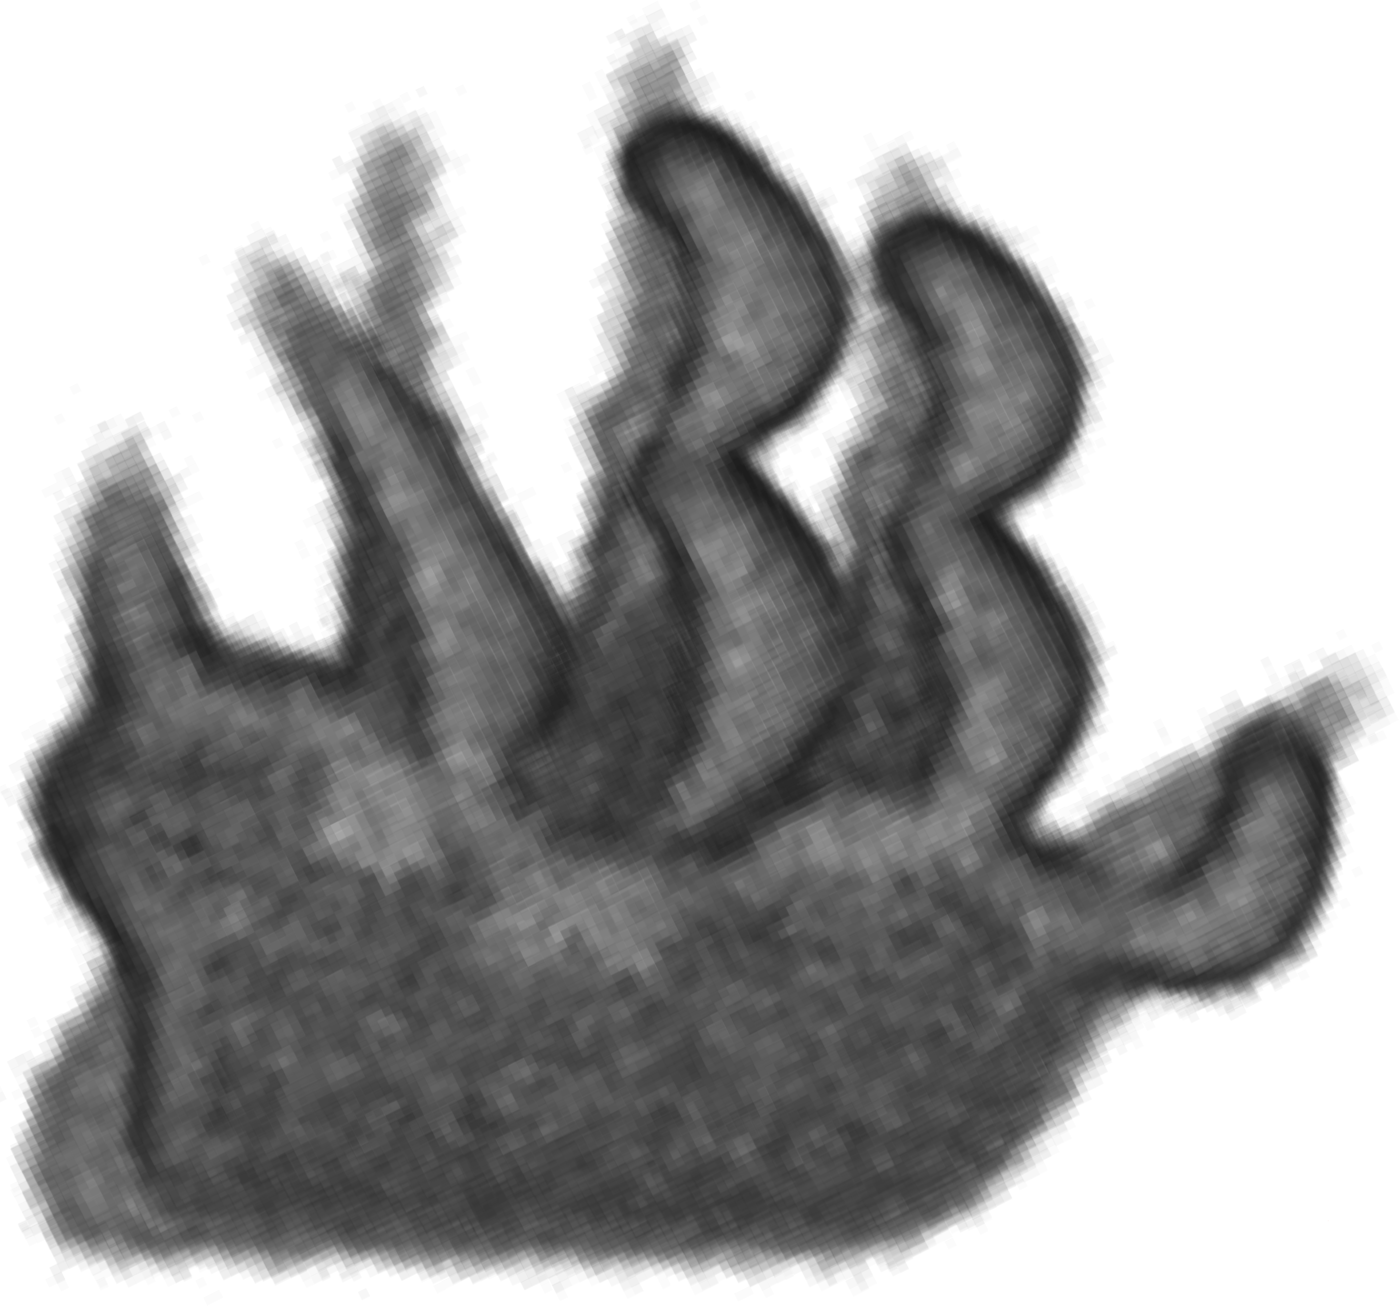
\includegraphics[width=1\linewidth]{./fig/eval/noise_high.png}
		\subcaption{$\sigma_{n} = 0.02L$}
		\label{fig/eval/noise_high}
	\end{subfigure}
	\caption{\textbf{Effect of sampling noise.} The ``galleon'' shape from the \meshset dataset with different levels of sampling noise.}
	\label{fig/eval/noisesample}
\end{figure}

% done
Sampling noise and density are crucial factors in 3D interest point detection. As most of the 3D data acquisition techniques rely on shape reconstruction from point clouds or tomograms, existing shape acquisition techniques, such as multi-view stereo and 3D ultrasound, often produce data with high signal-to-noise ratio. 

% done 
In the sampling noise test, different levels of Gaussian white noise, with standard deviations $\sigma_{n}$ from $0L$ to $0.03L$, were applied to the \meshset dataset. Figure \ref{fig/eval/noisesample} shows the effect of sampling noise to a sample shape, shape details features disappears gradually as sampling noise level increases. 
The quantitative experimental result is displayed in figure \ref{fig/eval/graph_noise}. MSER outperforms other interest points, demonstrating high robustness. While the $\areascore$ scores of other detectors declines rapidly, MSER still achieves a high $\areascore$ score. The DoH detector shows a relatively stronger tolerance than detectors like SURF, Harris and VFAST. In contrast, the SURF detector has almost no repeatable point when sampling noise becomes higher than $6.5\%L$.

\subsubsection{Sampling density}

% done
In this experiment, the $\areascore$ score of shapes with various sampling densities were measured. Point clouds were randomly sampled from the input meshes, with point cloud sizes ranging from $4000$ points to $405000$ points. The sampling density directly affected voxelisation process of the point clouds, loss of details and holes were observed in point clouds of low sampling densities. 

% done 
Figure \ref{fig/eval/graph_sample} presents the change of $\areascore$ scores versus point cloud size. The scores vary linearly in log scale, thus a diminishing return is observed with increasing sampling density. MSER achieves the best average performance but it also has the largest variance across different shapes. In addition, DoH and DoG produce satisfactory results, with high scores but smaller intra-dataset variance than that of MSER.

% done 
\begin{figure}[ht]
	\centering 
	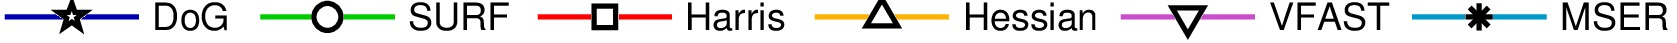
\includegraphics[width=0.70\linewidth]{./fig/eval/hlegend.jpg}
	\begin{subfigure}[t]{0.48\linewidth}
		\centering 
		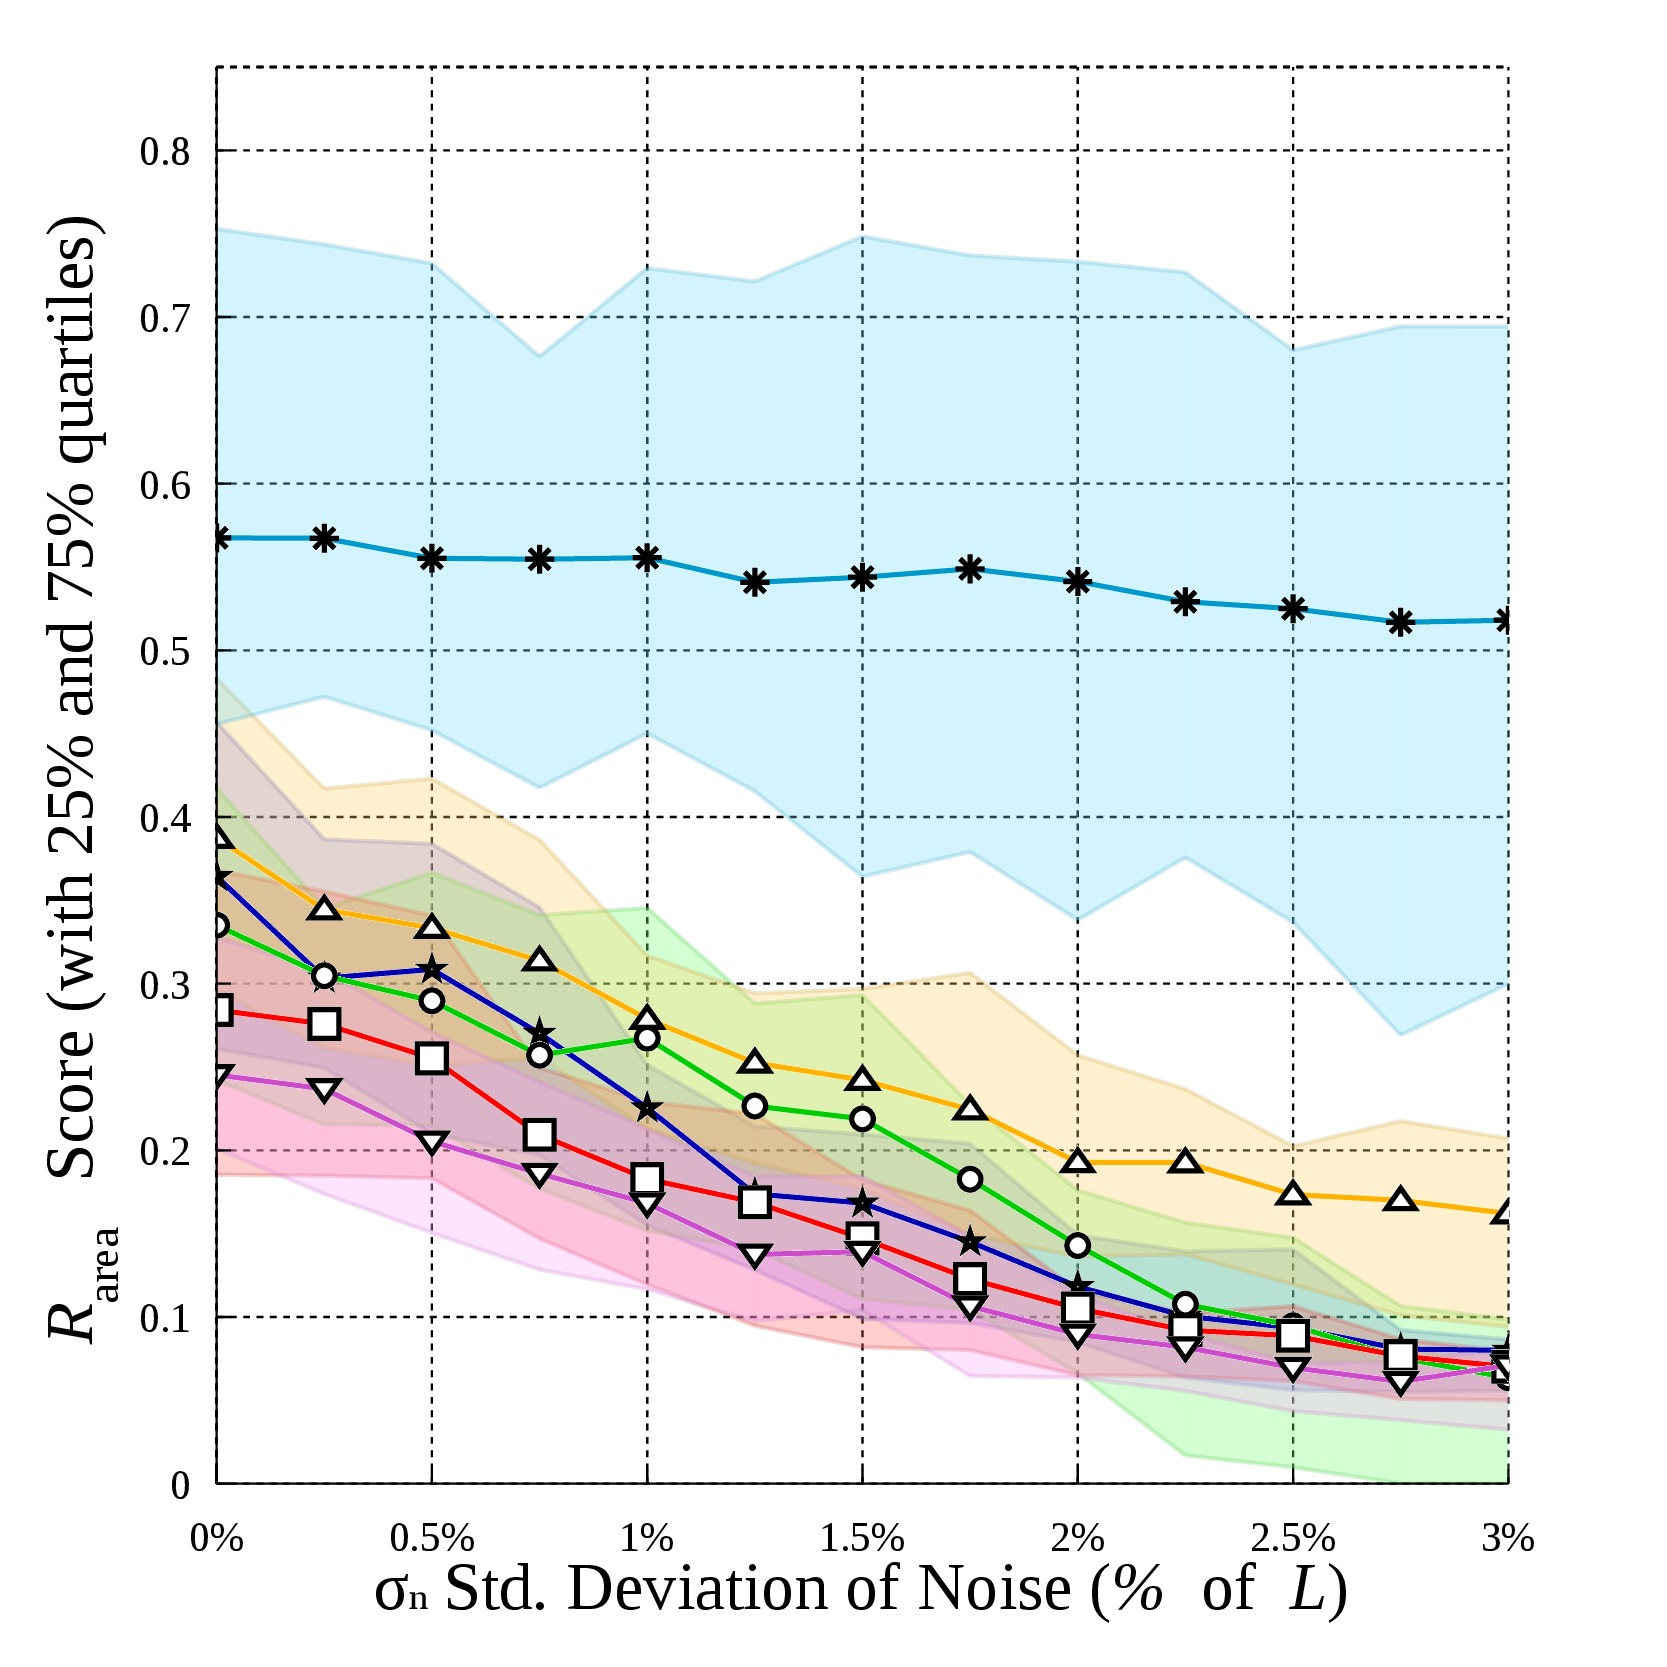
\includegraphics[width=1\linewidth]{./fig/eval/graph_noise.jpg}
		\subcaption{Sampling noise}
		\label{fig/eval/graph_noise}
	\end{subfigure}
	\begin{subfigure}[t]{0.48\linewidth}
		\centering 
		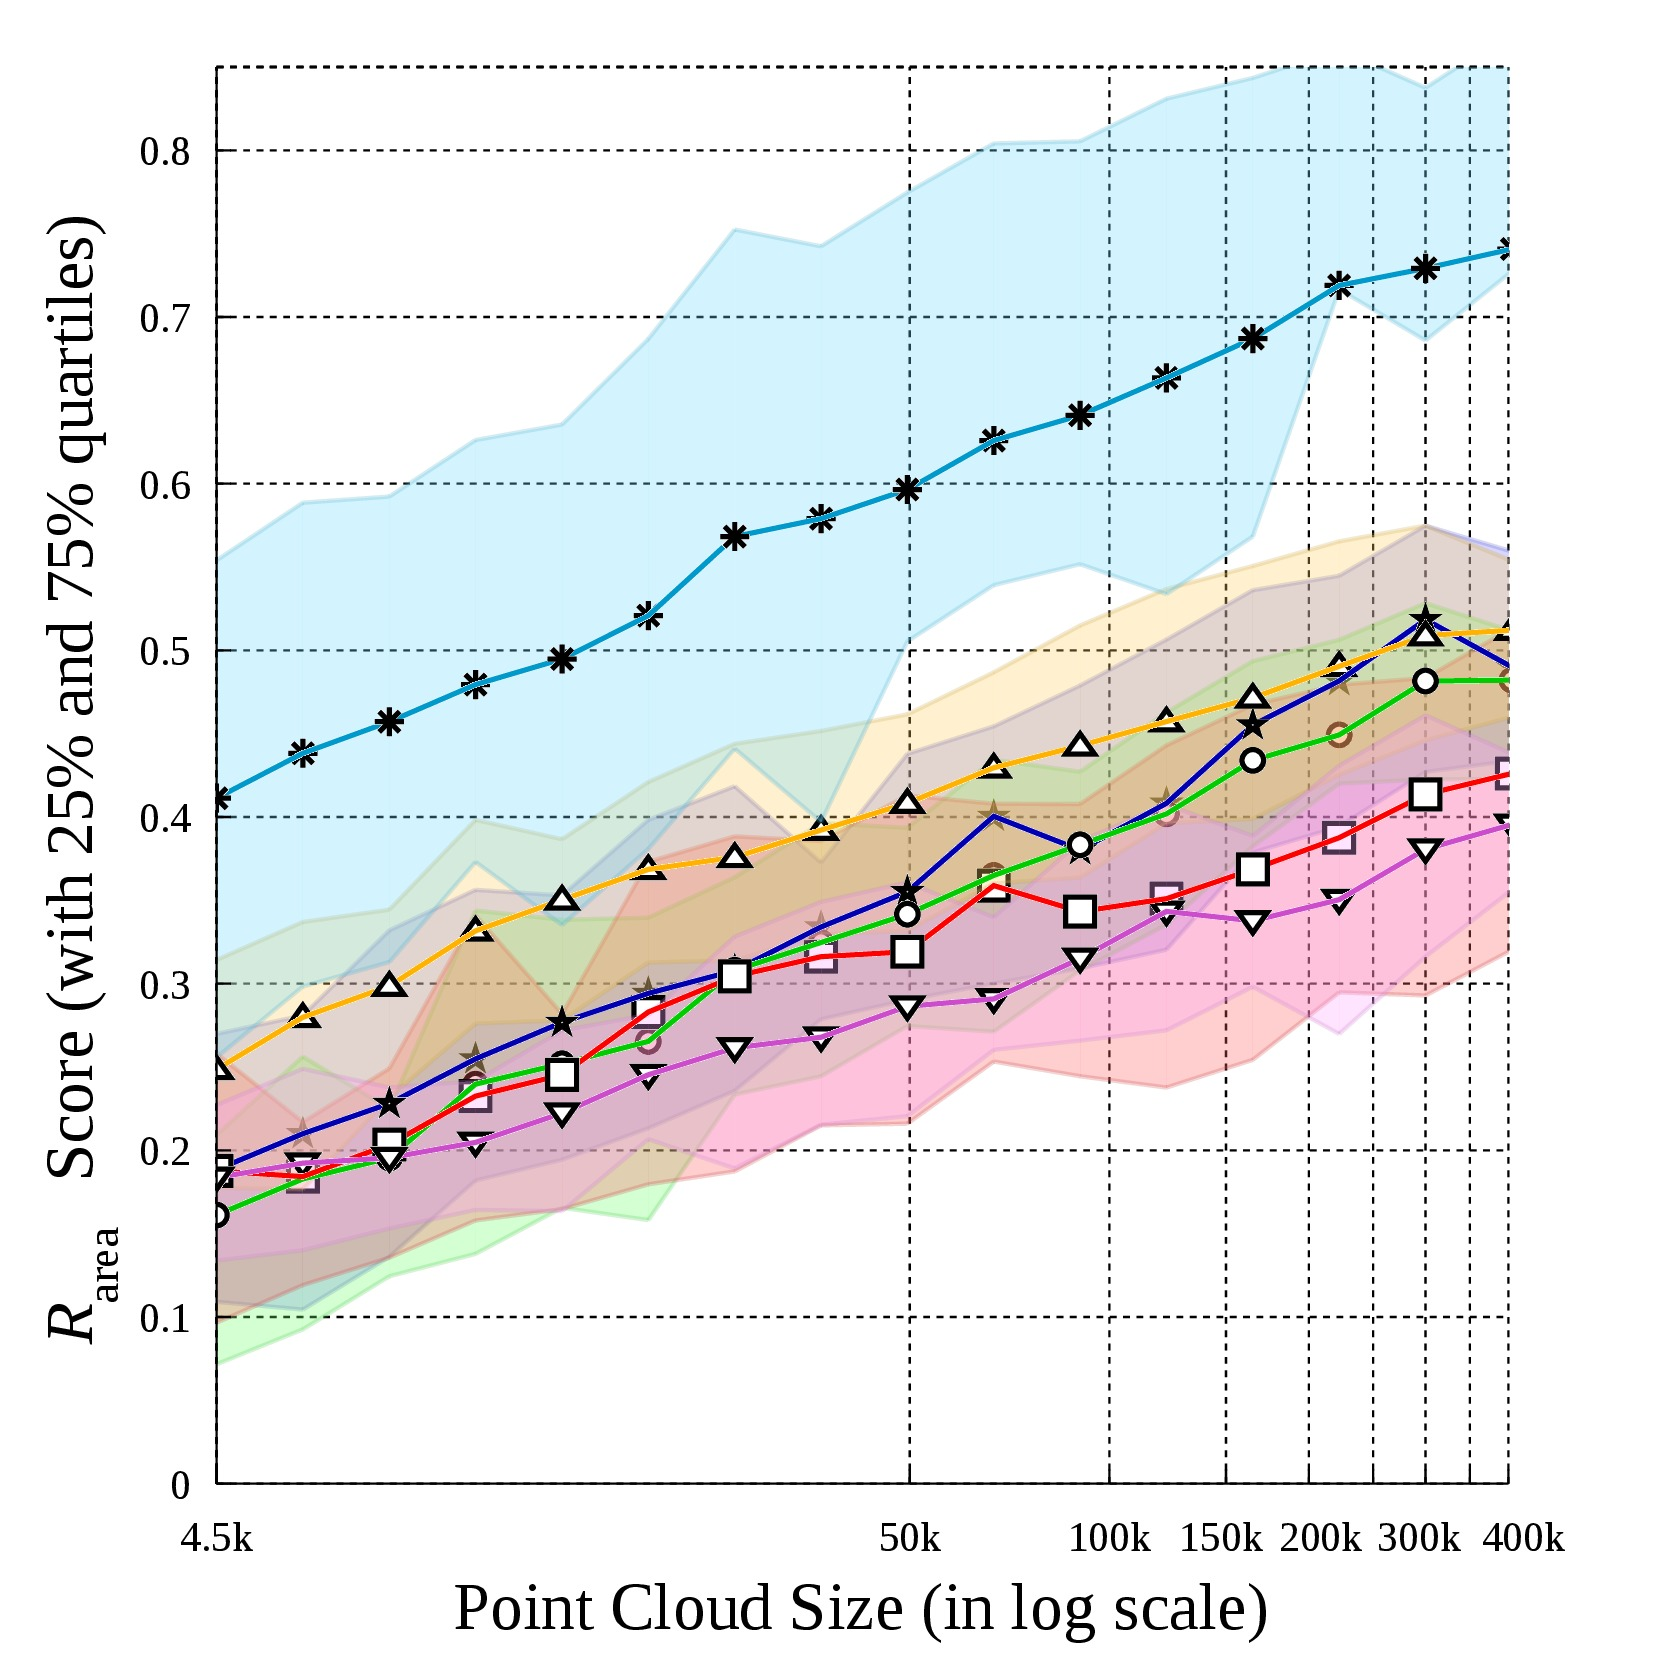
\includegraphics[width=1\linewidth]{./fig/eval/graph_sampling.jpg}
		\subcaption{Sampling density}
		\label{fig/eval/graph_sample}
	\end{subfigure}
	\caption{\textbf{$\areascore$ scores of the \meshset dataset.} Repeatability area scores under (a) sampling noise, (b) sampling density (point cloud size).}
	\label{fig/eval/graph_graph0} 
\end{figure}

\subsubsection{Rotation}

% done 
The robustness of the candidate detectors to rotational aliasing effects was evaluated in this experiment. For each step of rotation angle, an average $\areascore$ score was computed by matching the testing shapes multiple times using different rotation axes, making the evaluation results unbiased. Eight rotation axes were generated randomly for each shape, and rotations of increasing magnitude, up to $90^\circ$, were applied to them and then the reference shapes. 

% done 
The effect of rotation is shown in figure \ref{fig/eval/graph_rotation}. Most detectors show excellent tolerance to rotation, inheriting this from their image-based counterparts. 
DoG and MSER perform slightly better than others, with stable average $\areascore$ score over a wide range of rotation angles. SURF performs worse than other volumetric interest points because the use of box filters has introduced extra quantisation errors when the shapes are rotated.

\subsubsection{Scale}

% done 
In this experiment, dimensions of voxelised input data were scaled from $50\%$ to $200\%$ of their original sizes. In order to make an unbiased comparison, the transformed shapes were not directly interpolated from their voxelised reference shapes using interpolation. Rather, input point clouds were re-voxelised with varying volume dimensions $L$, whilst other parameters remained unchanged. 

% done 
Figure \ref{fig/eval/graph_scaling} illustrates the average $\areascore$ measured against different scale changes. 
From the experimental results, DoG and DoH detectors are relatively more robust to scale. SURF only works well at $100\%$ and its performance drops rapidly outside the original scale, because of the approximated scale-space used. MSER achieves the best result at its original size, but its performance drops steadily when the shape is resized.
Generally, repeatability scores of all detectors drop faster in down-sampled volumes (scale $< 100\%$) than in up-sampled volumes (scale $> 100\%$). 
This was because information content of smaller shape features was discarded when the input volumes were downsized.   
In addition, the scale-space did not cover any feature with a size smaller than the first octave, therefore fine details were undetected.  
Meanwhile, the performance of most detectors decreases slowly as scale increases, when some features have become too large to be detected. 
\begin{figure}[ht]
	\centering 
	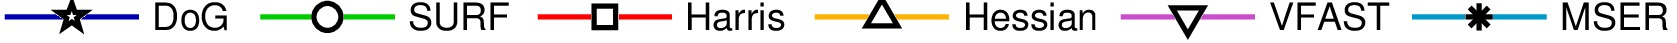
\includegraphics[width=0.70\linewidth]{./fig/eval/hlegend.jpg}
	\begin{subfigure}[t]{0.48\linewidth}
		\centering 
		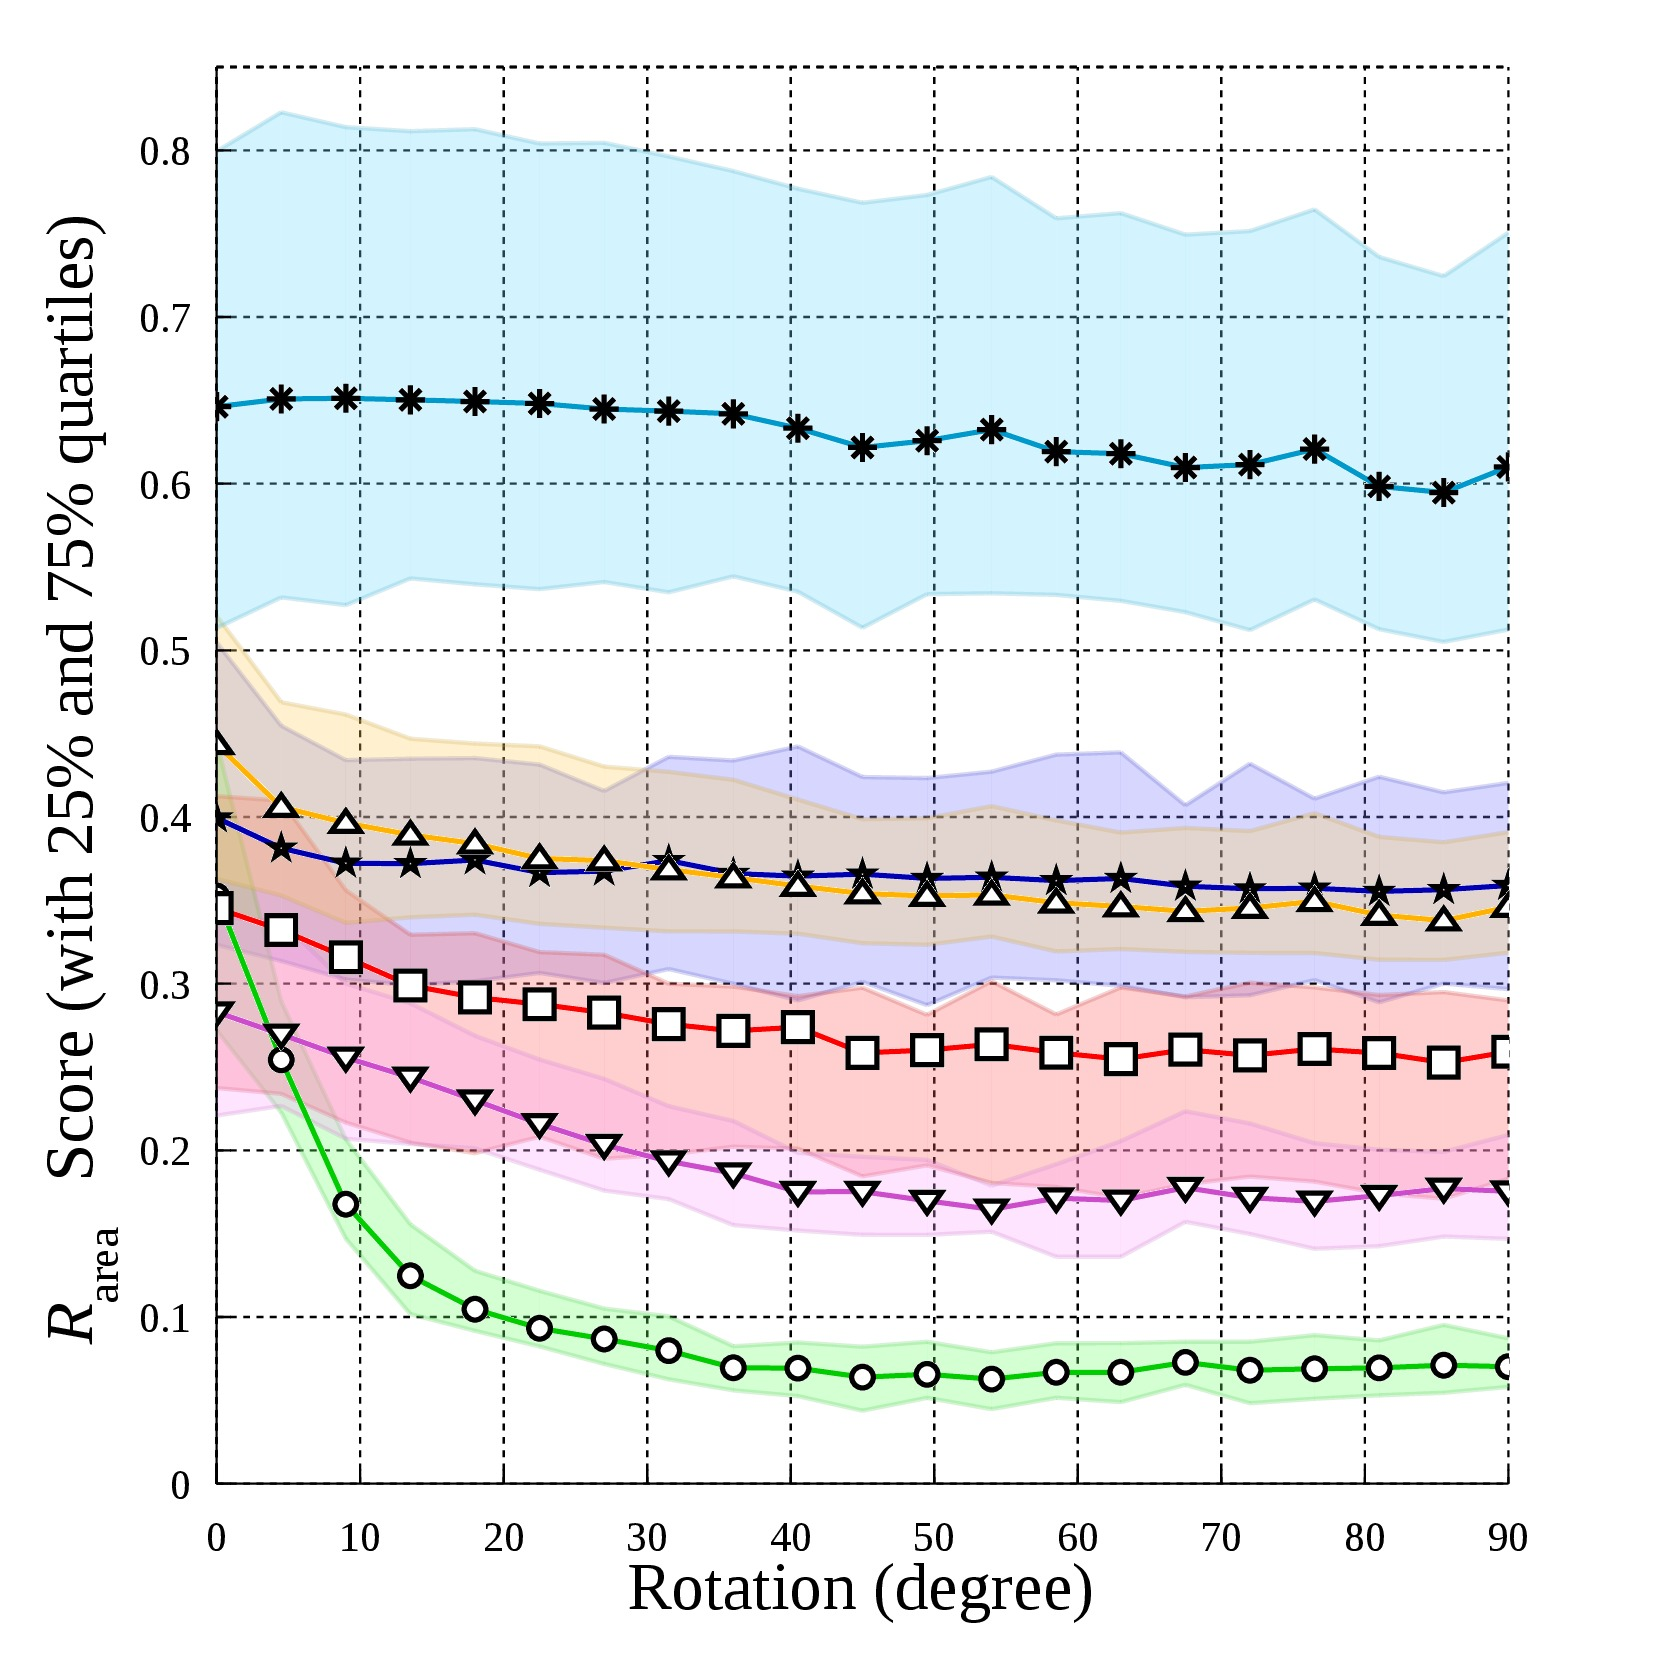
\includegraphics[width=1\linewidth]{./fig/eval/graph_rotation.jpg}
		\subcaption{Rotation}
		\label{fig/eval/graph_rotation}
	\end{subfigure}
	\begin{subfigure}[t]{0.48\linewidth}
		\centering 
		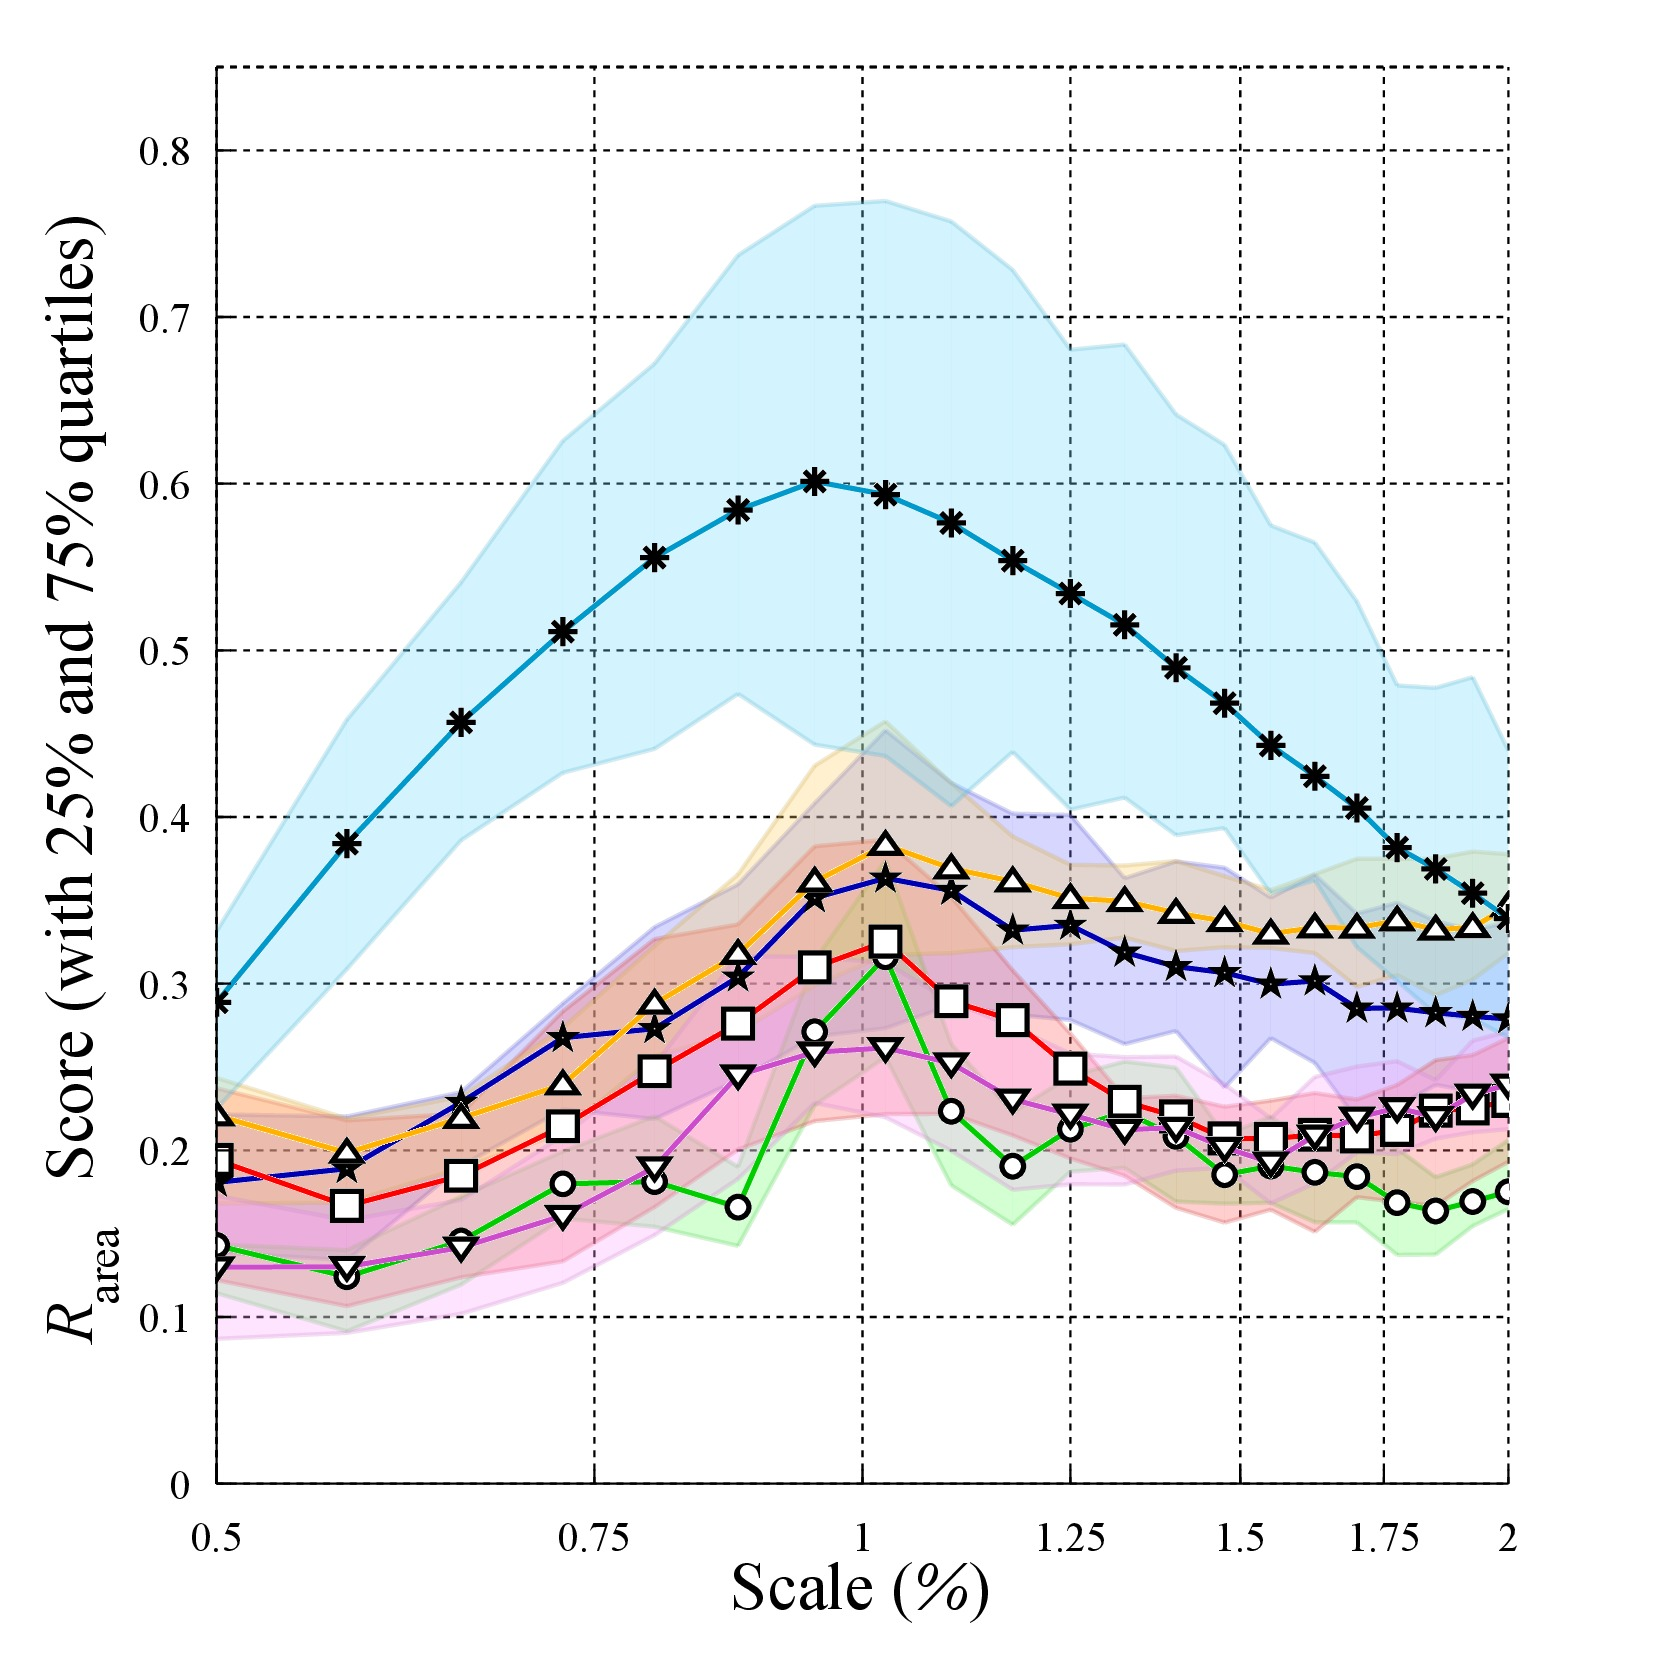
\includegraphics[width=1\linewidth]{./fig/eval/graph_scaling.jpg}
		\subcaption{Scale}
		\label{fig/eval/graph_scaling}
	\end{subfigure}
	\caption{\textbf{$\areascore$ scores of the \meshset dataset.} Repeatability area scores under varying (a) rotation, (b) scale.}
	\label{fig/eval/graph_graph1} 
\end{figure}

\subsubsection{Number of corresponding interest points}

Table \ref{tab/eval/numcorr} presents quantitative results for the number of interest points and correspondences at three noise levels ($0.0025L$, $0.01L$ and $0.02L$), \cf figure \ref{fig/eval/noisesample}.
The MSER detector obtains the highest percentage of correspondences, yet it produces a smaller set of interest points. By contrast, DoH, SURF and Harris give larger sets of interest points with good correspondence ratios. The displacement threshold used in this experiment ($\disp = 0.015L$) was about half the typical value, allowing only the highly accurate correspondences to be counted towards the values in the table. 

\begin{table}[ht]
	\centering
	\begin{tabular}{|cc|ccc|}
\hline
& & \multicolumn{3}{c}{\textbf{Sampling noise level}}  \\
& &  {\textbf{Low}}  & {\textbf{Medium}}  & {\textbf{High}}  \\
& & ($0.0025L$) & ($0.01L$) & ($0.02L$) \\
\hline
\hline
\multirow{3}{*}{DoG}  & Avg. \# Pts. &   122.0 & 118.2 & 73.1 \\
& Avg. \# Corr. &  48.8 & 35.1 &  9.3 \\
& (Corr. \%) & (\textit{39.8\%}) & (\textit{29.7\%}) & (\textit{12.7\%}) \\
\hline
\multirow{3}{*}{SURF} & Avg. \# Pts. & 154.7 & 70.4  & 28.7 \\
& Avg. \# Corr. &  54.7 & 18.4  & 3.84 \\
& (Corr. \%) &  (\textit{35.3\%}) & (\textit{26.2\%})  & (\textit{13.4\%}) \\
\hline
\multirow{3}{*}{Harris} & Avg. \# Pts. & 303.3 & 142.2 &  123.8 \\
& Avg. \# Corr. & 78.6  & 33.2  &    13.4  \\
& (Corr. \%) & (\textit{25.9\%}) & (\textit{23.3\%}) & (\textit{10.83\%}) \\
\hline
\multirow{3}{*}{DoH}& Avg. \# Pts. &  {\textbf{\color{blue}330.8}} & {\textbf{\color{blue}272.0}} &   {\textbf{\color{blue}201.2}} \\
& Avg. \# Corr. & {\textbf{\color{blue}117.1}} & {\textbf{\color{blue}72.2}}  &   {\textbf{\color{blue}30.2}} \\
& (Corr. \%) & (\textit{35.4\%}) & (\textit{26.6\%}) & (\textit{18.2\%}) \\
\hline
\multirow{3}{*}{VFAST}& Avg. \# Pts. &  115.9 &  85.5  &  74.6\\ 
& Avg. \# Corr. & 33.5  & 15.5  &    7.4 \\
& (Corr. \%) & (\textit{28.8\%}) & (\textit{18.10\%})  & (\textit{9.85\%}) \\
\hline
\multirow{3}{*}{MSER}& Avg. \# Pts.  &  99.0  & 74.4  &   52.5 \\
& Avg. \# Corr. & 59.9 & 44.7  &   28.8 \\
& (Corr. \%) & ({\textit{\textbf{\color{blue}60.5\%}}})  & ({\textit{\textbf{\color{blue}60.2\%}}})  & ({\textit{\textbf{\color{blue}54.9\%}}})\\
\hline
\end{tabular}
\caption{\textbf{Number of detected interest points.} For each row, from top to bottom: average number of interest points detected, average number of correspondence, percentage of corresponding interest point pairs.}
\label{tab/eval/numcorr}
\end{table}


\subsubsection{Saliency}

% done 
Figure \ref{fig/eval/graph_keypointnum} shows the repeatability ratio, $R_\textrm{ratio}$, with varying percentages of interest points. For each detector, interest points were detected and sorted by their corresponding saliency responses in descending order, afterwards the first $p\%$ of interest points were used to calculate $R_\mathrm{ratio}$. However, since no saliency measure has been defined in the MSER detector, the number of detected interest points could not be controlled directly; MSER was therefore not included in figure \ref{fig/eval/graph_keypointnum}. Similar to the previous test on correspondences, $R_\textrm{ratio}$ was computed using a smaller displacement threshold ($\disp = 0.015L$) in this experiment.   

% done 
The performances of DoG and Harris detectors tend to be stable, though Harris performs notably worse than DoG, with increasing numbers of interest points, \ie decreasing saliency threshold. The results imply that a saliency threshold is not necessary for these detectors. In other words, the saliencies of DoG and Harris do not reflect their potential repeatabilities. The performance of DoH, which are initially the best, decrease very slowly and converge with DoG and SURF, indicating that the lower saliency points are less reliable. A saliency threshold for DoH would benefit applications requiring more accurate point localisation. By contrast, the repeatability scores of SURF and VFAST increase steadily before levelling off, suggesting that some of the high saliency points are unreliable. Having an unstable saliency measure, this would pose more of a problem in terms of interest point selection. 

\begin{figure}[ht]
	\centering
	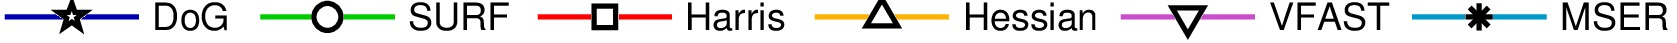
\includegraphics[width=0.70\linewidth]{./fig/eval/hlegend.jpg} \\ 
	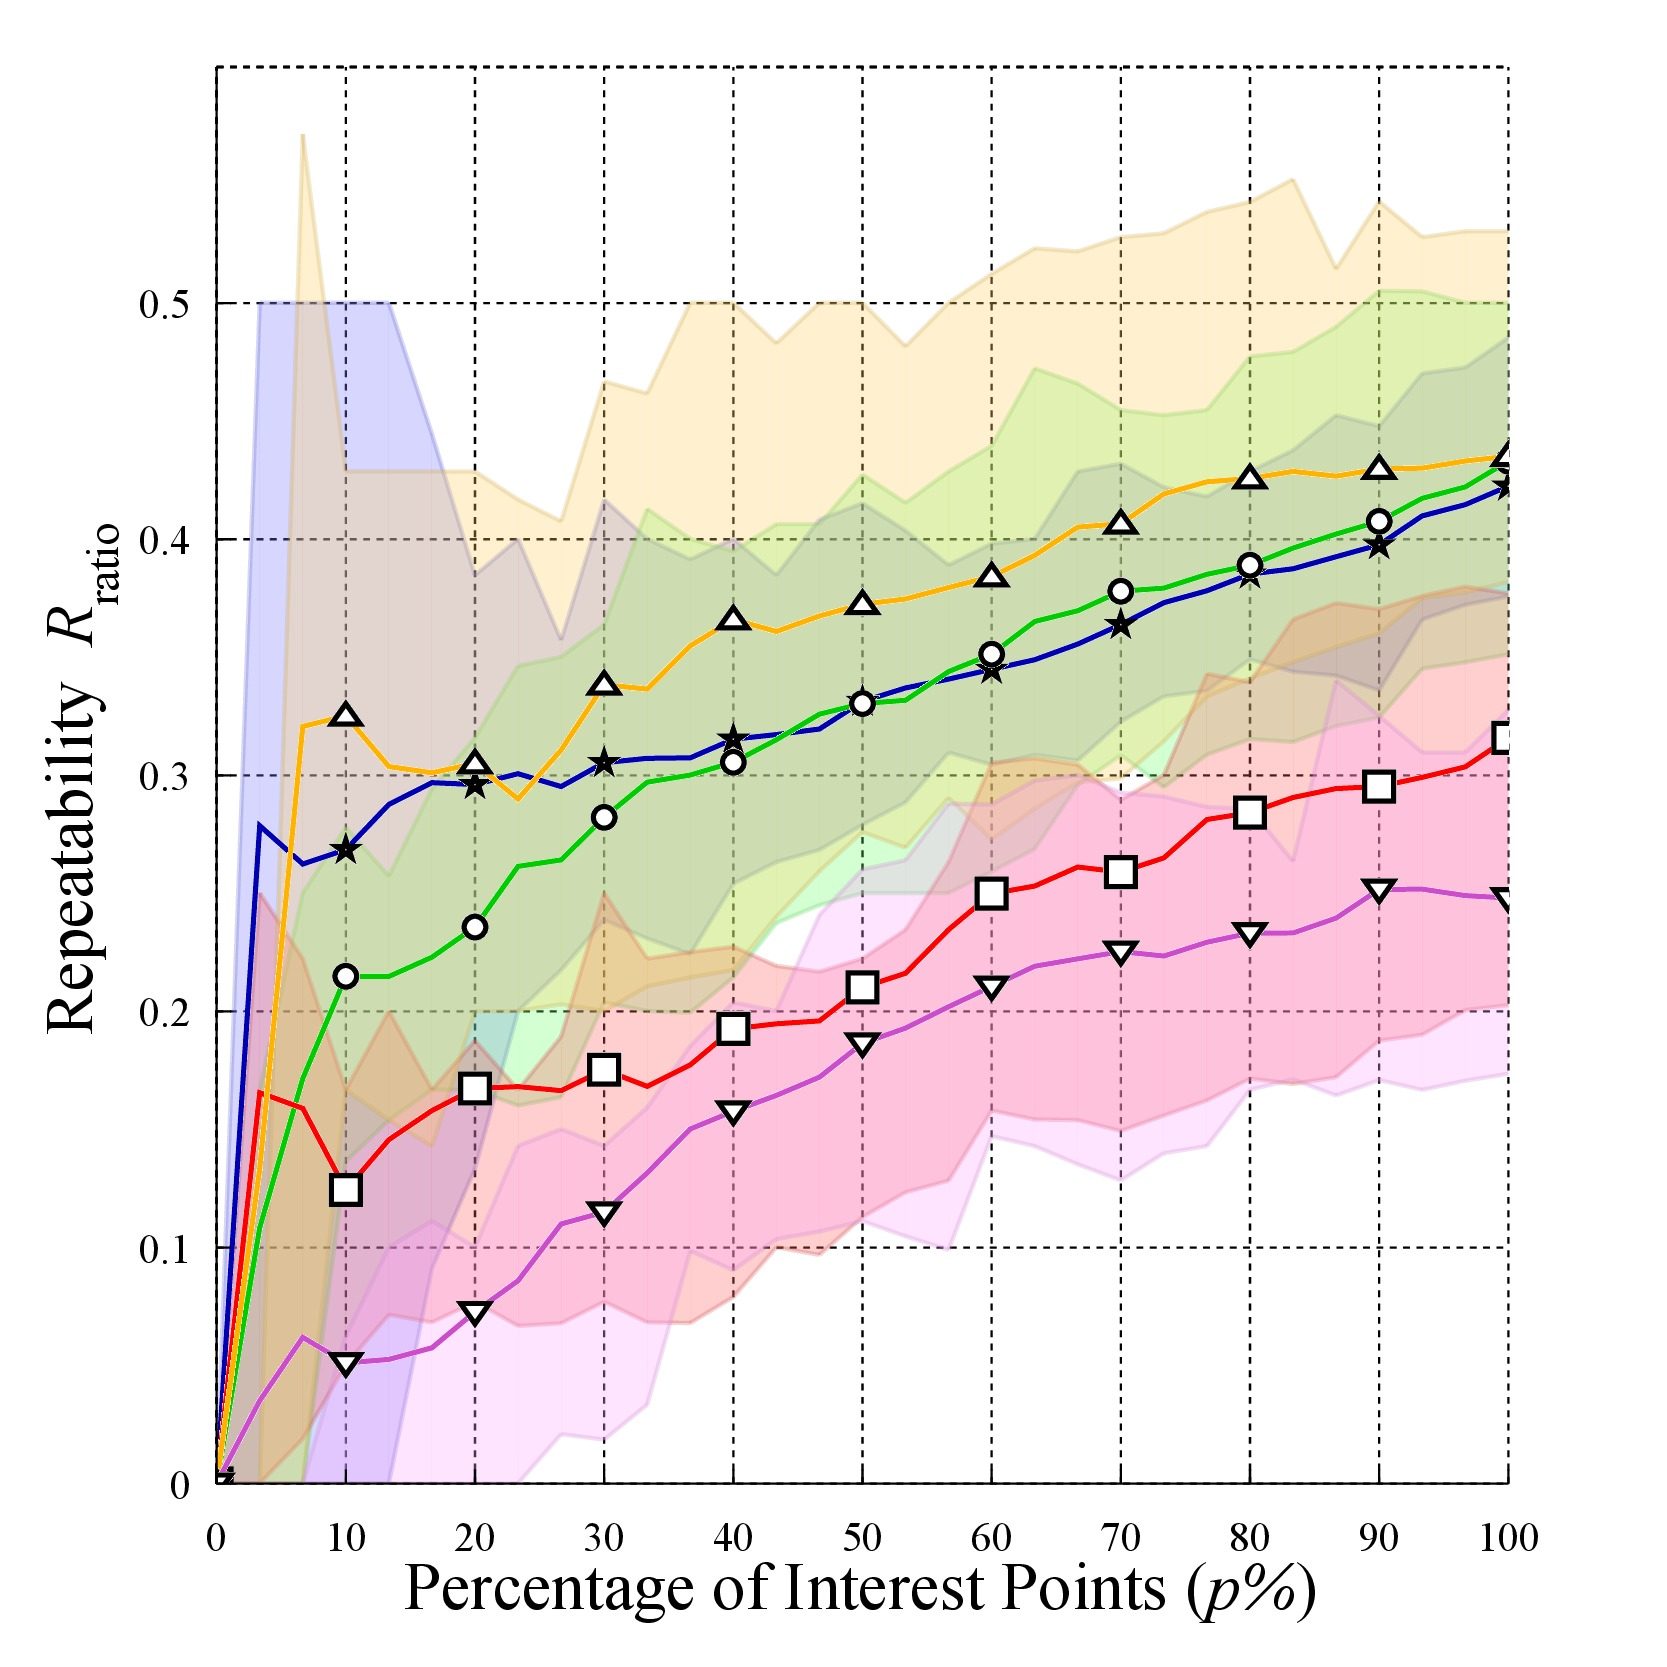
\includegraphics[width=0.48\linewidth]{./fig/eval/graph_keypointnum.jpg}
	\caption{\textbf{$\areascore$ scores of the \meshset dataset.} Repeatability area score under varying percentage of interest points.}
	\label{fig/eval/graph_keypointnum}	
\end{figure}

\subsection{Experiments on MRI and stereo data}

% done 
Interest points detectors were also evaluated on the \mriset and the \stereoset datasets. As a reference for cross validation, average scores obtained from the \meshset dataset are plotted against displacement threshold $\disp$ in figure \ref{fig/eval/graph_syn}. 

% done 
\subsubsection{MRI dataset} This dataset contains two MRI scans of a human brain, each MRI has the longest dimension $L$ of $218$ voxels.
Figure \ref{fig/eval/mri} shows the MSER interest points detected in the data. It is worth noting that some points detected on the MRIs are matched easily, such as those on the nose-tips, eye sockets and foreheads, but that there are fewer detections within the brain area, which consists of voxels with smaller, irregular intensity variations.

% done 
The $\areascore$ scores are measured from the \mriset dataset with varying $\disp$ in figure \ref{fig/eval/graph_mri}. The evaluation results are comparable to that of synthetic mesh data. MSER, DoG and DoH attain slightly better performances in synthetic meshes, while the Harris detector is good at detecting complicated internal structures in the MRI scans. 

\begin{figure}[ht]
	\centering 
	\begin{subfigure}[t]{0.35\linewidth} \centering 
		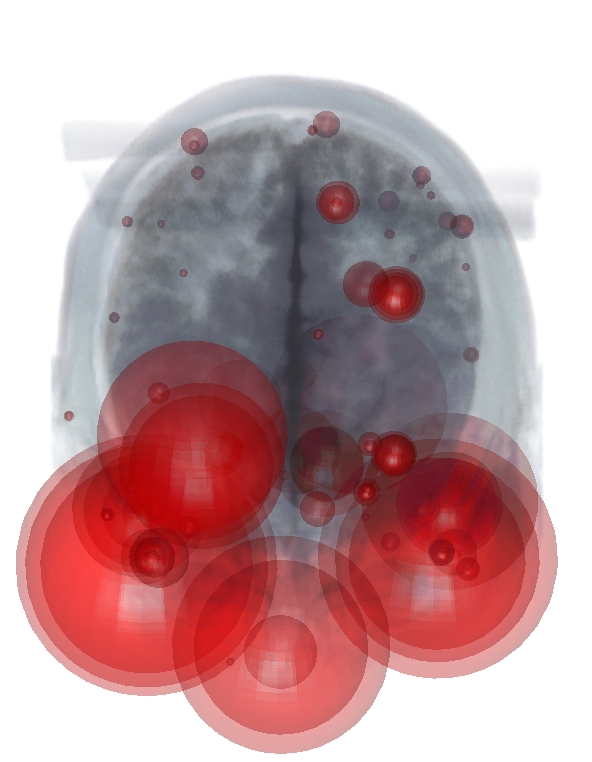
\includegraphics[width=0.8\linewidth]{./fig/eval/mri.png}
		\subcaption{MRI scan 1}
		\label{fig/eval/mri1}
	\end{subfigure}
	\begin{subfigure}[t]{0.35\linewidth} \centering 
		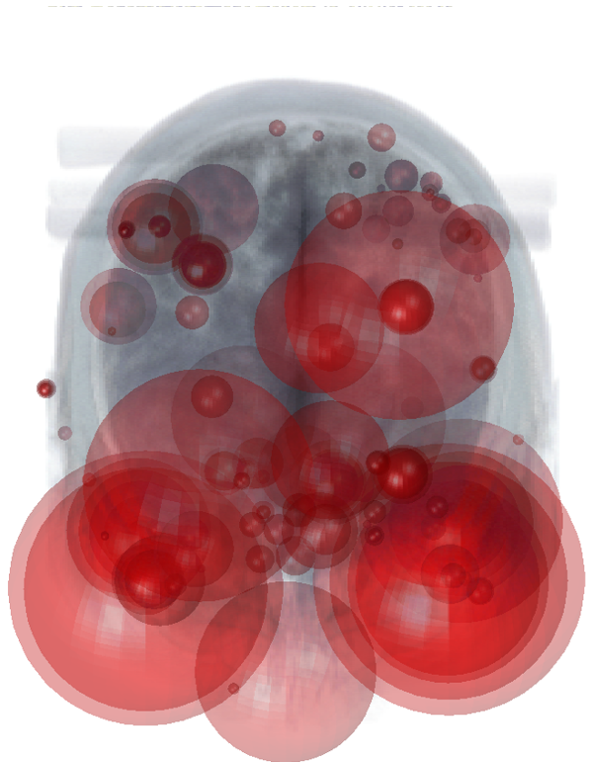
\includegraphics[width=0.8\linewidth]{./fig/eval/mri2.png}
		\subcaption{MRI Scan 2}
		\label{fig/eval/mri2}
	\end{subfigure}
	\caption{\textbf{Experiment on MRI data.} Two MRI scans of a human brain, with detected MSER features.}
	\label{fig/eval/mri}
\end{figure}

\subsubsection{Stereo dataset} 

\begin{figure}
	\centering
	\begin{subfigure}[t]{0.23\linewidth} \centering
		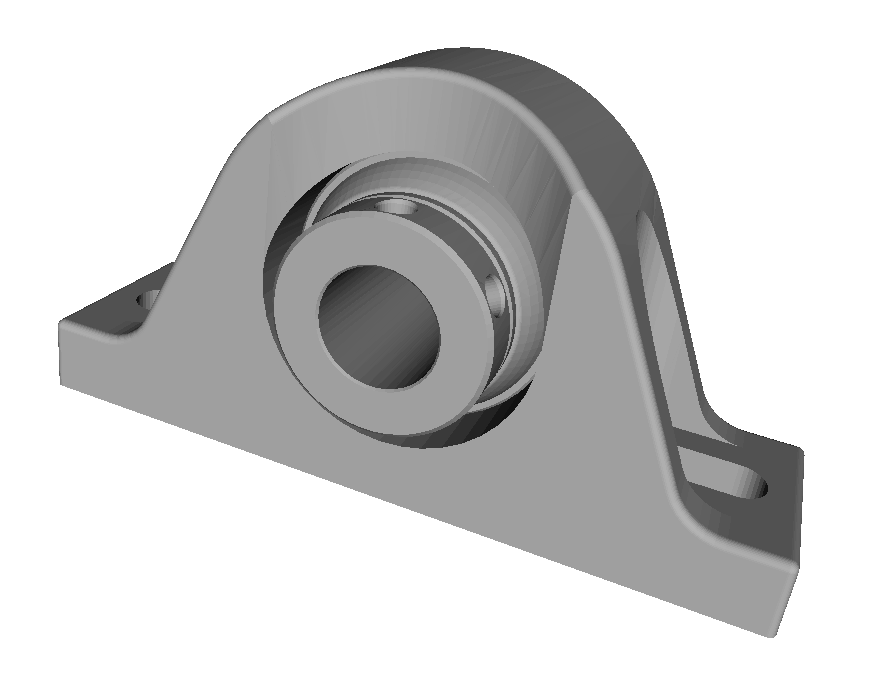
\includegraphics[width=1\linewidth]{./fig/eval/toshiba_bearing1.png}
		\subcaption{Bearing}
	\end{subfigure}
	\begin{subfigure}[t]{0.23\linewidth} \centering
		\includegraphics[width=0.8\linewidth]{./fig/eval/toshiba_bracket1.png}
		\subcaption{Bracket}
	\end{subfigure}
	\begin{subfigure}[t]{0.23\linewidth} \centering
		\includegraphics[width=1\linewidth]{./fig/eval/toshiba_flange1.png}
		\subcaption{Flange}
	\end{subfigure}
	\begin{subfigure}[t]{0.23\linewidth} \centering
		\includegraphics[width=1\linewidth]{./fig/eval/toshiba_knob1.png}
		\subcaption{Knob}
	\end{subfigure}
	\begin{subfigure}[t]{0.23\linewidth} \centering
		\includegraphics[width=1\linewidth]{./fig/eval/toshiba_mini1.png}
		\subcaption{Car}
	\end{subfigure}
	\begin{subfigure}[t]{0.23\linewidth} \centering
		\includegraphics[width=1\linewidth]{./fig/eval/toshiba_pipe1.png}
		\subcaption{Pipe}
	\end{subfigure}
	\begin{subfigure}[t]{0.23\linewidth} \centering
		\includegraphics[width=1\linewidth]{./fig/eval/toshiba_piston1.png}
		\subcaption{Piston 1}
	\end{subfigure}
	\begin{subfigure}[t]{0.23\linewidth} \centering
		\includegraphics[width=1\linewidth]{./fig/eval/toshiba_piston2.png}
		\subcaption{Piston 2}
	\end{subfigure}
	\caption{\textbf{Rendered CAD models of the \stereoset dataset.}} 
	\label{fig/eval/mvscad}
\end{figure}

% done 
Sixteen point clouds were captured using a multi-view stereo technique \cite{Vogiatzis2011} from realistic, 3D-printed CAD models. The point clouds were converted into volumes with maximum length $L$ of $132$ voxels. Figure \ref{fig/eval/mvscad} shows the CAD models from the \stereoset dataset; figure \ref{fig/eval/mvs} visualises different types of interest points detected on their corresponding voxelised shapes.

% done 
The $\areascore$ scores obtained from the \stereoset dataset, shown in figure \ref{fig/eval/graph_mvs}, are lower compared with the \meshset and the \mriset datasets, especially at a small matching threshold $\disp$. Nonetheless, in terms of overall rankings and relative scores of the detectors, synthetic and real data show similar behaviours. The decrease in performance for stereo data are due to its: (a) low sampling frequency and high noise, (b) uneven object surfaces, which are infeasible for blob detection algorithms, such as MSER, SURF and DoH, and (c) small errors in the estimated ground truth poses from ICP alignment.
The differences in $\areascore$ scores are due to occlusions, viewpoint changes and uneven sampling density of the \stereoset dataset. 

% done 
Some testing instances, \eg ``car'' in figure \ref{fig/eval/mvs}, have much sparser point clouds due lack of texture on the surface, but the distribution of detected features is no less dense across any of the detectors, suggesting that the experimental results of the synthetic datasets are representative of sparse point clouds as well as dense ones.

\begin{figure}[ht]
	\centering
	\includegraphics[width=0.80\linewidth]{./fig/eval/hlegend.jpg}\\
	\begin{subfigure}[t]{0.49\linewidth}
		\centering 
		\includegraphics[width=0.95\linewidth]{./fig/eval/graph_oneshape.jpg}
		\subcaption{$\areascore$ score: \meshset}		
		\label{fig/eval/graph_syn}
	\end{subfigure}
	\begin{subfigure}[t]{0.49\linewidth}
		\centering 
		\includegraphics[width=0.95\linewidth]{./fig/eval/graph_mri.jpg}
		\subcaption{$\areascore$ score: \mriset}		
		\label{fig/eval/graph_mri}
	\end{subfigure}
	\begin{subfigure}[t]{0.49\linewidth}
		\centering 
		\includegraphics[width=0.95\linewidth]{./fig/eval/graph_stereo.jpg}
		\subcaption{$\areascore$ score: \stereoset}		
		\label{fig/eval/graph_mvs}
	\end{subfigure}
	\caption{\textbf{$\areascore$ scores versus displacement threshold $d$.} Left to right: (a) the \meshset dataset, (b) the \mriset dataset and (c) the \stereoset dataset.}
\label{fig/eval/graph2}
\end{figure}

\subsection{Run-time performance}

% done
Computation efficiency is also a crucial factor for choosing a suitable interest point detector for different computer vision applications. Since the storage size of volumetric data is usually much larger than 2D images, time and memory complexities of the interest point detectors increase accordingly. Operations which are considered efficient for 2D images can become much slower for 3D volumetric data. For non-volumetric input data such as point clouds, extra computation time is required to voxelise the shape. 

% done 
Some interest point detectors can also be accelerated by parallel processing techniques, using specialised hardware such as GPUs and FPGAs \cite{Sinha2006, Cornelis2008, Teixeira2008, Bhatia2007, Dohi2011, Kristensen2007}. Table \ref{tab/eval/speedtable} summarises the algorithmic complexities of the candidate detectors and the time required for them to compute interest points on the \meshset dataset. From left to right, it lists (1) the algorithmic complexities, (2) the average processing time for the \meshset dataset, (3) potential parallel implementations and (4) existing machine learning-based acceleration. 
In order to facilitate a fair evaluation framework, all candidate detectors were implemented in MATLAB, without any hardware acceleration. The experiments were performed on the same hardware platform (Intel Core i7, $12$GB RAM). 

\begin{table}
\centering
\begin{tabular}{|c|cccc|}
\hline
\textbf{Interest} & \textbf{Complexity} & \textbf{Speed} & \textbf{Parallelisable} & \textbf{Machine} \\
\textbf{Point} & & \textbf{(\bm{$\mu$}s / voxel)} & & \textbf{learning} 	\\ 	
\hline
DoG 		& $O(SN)$ 			& $1.325 $ 			& \checkmark \cite{Sinha2006} & \\
SURF 		& $O(SN)$ 			& $1.035 $ 			& \checkmark \cite{Cornelis2008} & \\
Harris 		& $O(SN)$ 			& $1.112 $ 			& \checkmark \cite{Teixeira2008} & \\
DoH			& $O(SN)$ 			& $1.325 $ 			& \checkmark \cite{Bhatia2007} \\
VFAST 		& $O(SN)$ 			& $1.670 $ 			& \checkmark \cite{Dohi2011} & \checkmark \cite{Rosten2010}\\
MSER 		& $O(N\log(\log(N)))$ 	& $2.070 $ 			& \checkmark \cite{Kristensen2007} &\\
\hline
\end{tabular}
\caption{\textbf{Run-time performances of the candidate detectors.} $N$ denotes the number of voxels and $S$ is the number of octaves in the scale-space.}
\label{tab/eval/speedtable}
\end{table}

% done 
Theoretically, all detectors have a similar time complexity, except for MSER, which does not implement a Gaussian scale-space. The SURF detector is the fastest among the candidate detectors, as it uses Haar wavelets to accelerate the computation of Gaussian derivatives. Harris also shows high efficiency due to its relatively simple algorithm. MSER is the slowest detector, as its search algorithm for stable regions is less efficient in 3D volumes than in 2D images. Surprisingly, VFAST detector is the second slowest detector in the experiment. Since FAST is a pixel/voxel-wise rule based algorithm, the accelerated segment test in equation \ref{eqn/eval/fastast} cannot utilise the high performance linear algebra routines used by other detectors, such as separable filtering in DoG and SURF. VFAST detector can be accelerated by learning a decision tree classifier from training data \cite{Rosten2010}, which was not implemented in this experiment.

% done
\subsection{Qualitative analysis: blobs versus corners}
The candidate 3D interest point detectors can be roughly classified into three different categories: region-based blob detection (MSER), derivative-based blob detection (DoG, DoH and SURF) and corner detection (Harris, VFAST). The quantitative evaluation results suggest that region-based blob detectors work better than derivative-based blob detectors, and blob detectors are better than corner detectors, but 3D interest points cannot be evaluated by repeatability only. The candidate detectors also have different behaviours in terms of locations and scales of the interest points. Therefore, besides repeatability, it is also important to analyse the characteristics of detectors qualitatively. Figure \ref{fig/eval/mesh} visualises interest points, detected by the six candidate detectors, on the four sample shapes from the \meshset dataset.

% done 
\subsubsection{Region-based blob detection} MSER detects contiguous regions of any shape, \ie not limited to spherical blobs, allowing it to select more robust regions from a greater selection, and hence perform better. MSER performs well in 3D shape data because the shapes of salient regions are inherently less susceptible to viewpoint changes. It can be seen in figures \ref{fig/eval/mesh/mser} and \ref{fig/eval/mvs/mser} that MSER finds features at fewer locations, but over multiple scales. The locations tend to centre on regions of high surface curvature.

% done 
\subsubsection{Derivative-based blob detection} Theoretically, DoG, DoH and SURF find, in order of preference, spherical blobs, corners and planes. From the experimental results, DoG and DoH give qualitatively similar output, as shown in figures \ref{fig/eval/mesh/dog}, \ref{fig/eval/mvs/dog}, \ref{fig/eval/mesh/hessian} and \ref{fig/eval/mvs/hessian}, finding features such as limb extremities in the \meshset dataset, or sharp corners in the \stereoset dataset, as well as inside shape such as the hull of ``galleon'' and the hole in ``knob''. By contrast, SURF, despite being an approximation of the DoH detector, produces features off the surface (both inside and outside), often over regions of low surface curvature, as shown in figure \ref{fig/eval/testshapes/surf}. Instead of highly repeatable features, derivative-based approaches produce more diverse features than region-based detectors. Finally, their repeatability scores degrade more rapidly than MSER for noisy input data in figure \ref{fig/eval/graph_noise}, mainly due to higher rates of false positive detections. 


\subsubsection{Corner detection} Harris and VFAST both aim to find areas of high curvature. However, their outputs (figures \ref{fig/eval/testshapes/harris} and \ref{fig/eval/testshapes/fast}) varied qualitatively, with the former tending to find fewer features and more sharp corners than the latter, which finds an even distribution of features over both scale and location. In general, corner detection approaches are relatively less robust to noise and transformations than blob detection techniques. Whilst blobs remain stable in noisy or transformed volumetric data, small scale features like corners are more easily affected by quantisation errors or sampling noise. 
The performance of blob detectors dropped faster than that of edge detectors at low (figure \ref{fig/eval/graph_sample}) and uneven (figures \ref{fig/eval/graph_syn} and \ref{fig/eval/graph_mvs}) sampling densities. Holes form on shape surfaces in these situations, creating false positives for both corner and blob detectors, however, the detection of true positives appear to be more robust for corner detectors in these cases. 
% Comparing the \meshset dataset and the \stereoset dataset, blob detectors have a greater drop in $\areascore$ score than corner detectors. It is because holes are formed on shape surfaces at a low or uneven sampling density, \eg \stereoset dataset in figure \ref{fig/eval/mvs}, they prevent the formation of stable blobs inside the cavities of a shape as in the \meshset dataset (figure \ref{fig/eval/mesh}). On the other hand, corner features are mainly detected at edges where the sampling density is generally higher than shape surfaces, thus they are less affected. Nevertheless, the unevenly sampled surface create false positives for all detectors, an overall drop in $\areascore$ score is therefore observed in \ref{fig/eval/mvs}. 
%Holes are formed on the shapes' surfaces at a low or uneven sampling density, \eg \stereoset dataset in figure \ref{fig/eval/graph_mvs}, creating false positives for both corner and blob detectors. These holes also prevents the formation of larger blobs. However, detection of corner features, which are usually smaller in size than blobs, are less affected. 
%On the other hand, since corner-based detectors use smaller local windows than blob-based methods, they are feasible for detecting interest points when blobs cannot be detected correctly in low sampling density (\emph{c.f.} figure \ref{fig/eval/graph_mvs}).

\begin{figure}[ht]
	\centering
	\begin{subfigure}[t]{1\linewidth}\centering
		\makebox[0.15\linewidth]{}
		\makebox[0.175\linewidth]{\textbf{Bicycle}}
		\makebox[0.155\linewidth]{\textbf{Kicking man}}
		\makebox[0.175\linewidth]{\textbf{Galleon}}
		\makebox[0.175\linewidth]{\textbf{Ant}}
	\end{subfigure}
	\begin{subfigure}[t]{1\linewidth} \centering 
		\phantomcaption 
		\label{fig/eval/mesh/input}	
		\makebox[0.15\linewidth]{\raisebox{0.07\linewidth}{(a) Input}} 
		\includegraphics[width=0.175\linewidth]{./fig/eval/cycle_input.jpg} 
		\includegraphics[width=0.155\linewidth]{./fig/eval/guy_input.jpg} 
		\includegraphics[width=0.175\linewidth]{./fig/eval/ship_input.jpg}
		\includegraphics[width=0.175\linewidth]{./fig/eval/ant_input.jpg} 
	\end{subfigure}
	\begin{subfigure}[t]{1\linewidth} \centering 
		\phantomcaption 
		\label{fig/eval/mesh/dog}	
		\makebox[0.15\linewidth]{\raisebox{0.07\linewidth}{(b) DoG}} 
		\includegraphics[width=0.175\linewidth]{./fig/eval/cycle_dog.jpg} 
		\includegraphics[width=0.155\linewidth]{./fig/eval/guy_dog.jpg} 
		\includegraphics[width=0.175\linewidth]{./fig/eval/ship_dog.jpg}
		\includegraphics[width=0.175\linewidth]{./fig/eval/ant_dog.jpg} 
	\end{subfigure}
	\begin{subfigure}[t]{1\linewidth} \centering 
		\phantomcaption 
		\label{fig/eval/mesh/surf}	
		\makebox[0.15\linewidth]{\raisebox{0.07\linewidth}{(c) SURF}} 
		\includegraphics[width=0.175\linewidth]{./fig/eval/cycle_surf.jpg} 
		\includegraphics[width=0.155\linewidth]{./fig/eval/guy_surf.jpg} 
		\includegraphics[width=0.175\linewidth]{./fig/eval/ship_surf.jpg}
		\includegraphics[width=0.175\linewidth]{./fig/eval/ant_surf.jpg} 
	\end{subfigure}
	\begin{subfigure}[t]{1\linewidth} \centering 
		\phantomcaption 
		\label{fig/eval/mesh/harris}	
		\makebox[0.15\linewidth]{\raisebox{0.07\linewidth}{(d) Harris}} 
		\includegraphics[width=0.175\linewidth]{./fig/eval/cycle_harris.jpg} 
		\includegraphics[width=0.155\linewidth]{./fig/eval/guy_harris.jpg} 
		\includegraphics[width=0.175\linewidth]{./fig/eval/ship_harris.jpg}
		\includegraphics[width=0.175\linewidth]{./fig/eval/ant_harris.jpg} 
	\end{subfigure}
	\begin{subfigure}[t]{1\linewidth} \centering 
		\phantomcaption 
		\label{fig/eval/mesh/hessian}	
		\makebox[0.15\linewidth]{\raisebox{0.07\linewidth}{(e) DoH}} 
		\includegraphics[width=0.175\linewidth]{./fig/eval/cycle_hessian.jpg} 
		\includegraphics[width=0.155\linewidth]{./fig/eval/guy_hessian.jpg} 
		\includegraphics[width=0.175\linewidth]{./fig/eval/ship_hessian.jpg}
		\includegraphics[width=0.175\linewidth]{./fig/eval/ant_hessian.jpg} 
	\end{subfigure}
	\begin{subfigure}[t]{1\linewidth} \centering 
		\phantomcaption 
		\label{fig/eval/mesh/fast}	
		\makebox[0.15\linewidth]{\raisebox{0.07\linewidth}{(f) VFAST}} 
		\includegraphics[width=0.175\linewidth]{./fig/eval/cycle_fast.jpg} 
		\includegraphics[width=0.155\linewidth]{./fig/eval/guy_fast.jpg} 
		\includegraphics[width=0.175\linewidth]{./fig/eval/ship_fast.jpg}
		\includegraphics[width=0.175\linewidth]{./fig/eval/ant_fast.jpg} 
	\end{subfigure}
	\begin{subfigure}[t]{1\linewidth} \centering 
		\phantomcaption 
		\label{fig/eval/mesh/mser}	
		\makebox[0.15\linewidth]{\raisebox{0.07\linewidth}{(g) MSER}} 
		\includegraphics[width=0.175\linewidth]{./fig/eval/cycle_mser.jpg} 
		\includegraphics[width=0.155\linewidth]{./fig/eval/guy_mser.jpg} 
		\includegraphics[width=0.175\linewidth]{./fig/eval/ship_mser.jpg}
		\includegraphics[width=0.175\linewidth]{./fig/eval/ant_mser.jpg} 
	\end{subfigure}
	\caption{(a) Sample point clouds obtained from the Mesh dataset, (b) DoG, (c) SURF (d) Harris, (e) DoH, (f) V-FAST and (g) MSER, visualized on the voxelized data. The color spheres represent the positions and relative scales of the detected interest points.}
	\label{fig/eval/mesh}
\end{figure}


\begin{figure}[ht]
	\centering 
	\begin{subfigure}[t]{1\linewidth} \centering
		\makebox[0.15\linewidth]{}
		\makebox[0.180\linewidth]{\textbf{Car}}
		\makebox[0.180\linewidth]{\textbf{Bearing}}
		\makebox[0.180\linewidth]{\textbf{Knob}}
		\makebox[0.180\linewidth]{\textbf{Bracket}}
	\end{subfigure}
	\begin{subfigure}[t]{1\linewidth} \centering
		\phantomcaption 
		\label{fig/eval/mvs/input}
		\makebox[0.15\linewidth]{\raisebox{0.07\linewidth}{(a) Input}}		
		\includegraphics[width=0.180\linewidth]{./fig/eval/mini_input.jpg}
		\includegraphics[width=0.180\linewidth]{./fig/eval/bearing_input.jpg} 
		\includegraphics[width=0.180\linewidth]{./fig/eval/knob_input.jpg} 
		\includegraphics[width=0.180\linewidth]{./fig/eval/bracket_input.jpg} 
	\end{subfigure}
	\begin{subfigure}[t]{1\linewidth} \centering
		\phantomcaption 
		\label{fig/eval/mvs/dog}
		\makebox[0.15\linewidth]{\raisebox{0.07\linewidth}{(b) DoG}} 
		\includegraphics[width=0.180\linewidth]{./fig/eval/mini_dog.jpg} 
		\includegraphics[width=0.180\linewidth]{./fig/eval/bearing_dog.jpg}  
		\includegraphics[width=0.180\linewidth]{./fig/eval/knob_dog.jpg} 
		\includegraphics[width=0.180\linewidth]{./fig/eval/bracket_dog.jpg} 
	\end{subfigure}
	\begin{subfigure}[t]{1\linewidth} \centering
		\phantomcaption 
		\label{fig/eval/mvs/surf}
		\makebox[0.15\linewidth]{\raisebox{0.07\linewidth}{(c) SURF}}		
		\includegraphics[width=0.180\linewidth]{./fig/eval/mini_surf.jpg} 
		\includegraphics[width=0.180\linewidth]{./fig/eval/bearing_surf.jpg}  
		\includegraphics[width=0.180\linewidth]{./fig/eval/knob_surf.jpg} 
		\includegraphics[width=0.180\linewidth]{./fig/eval/bracket_surf.jpg} 
	\end{subfigure}
	\begin{subfigure}[t]{1\linewidth} \centering
		\phantomcaption 
		\label{fig/eval/mvs/harris}
		\makebox[0.15\linewidth]{\raisebox{0.07\linewidth}{(d) Harris}}		
		\includegraphics[width=0.180\linewidth]{./fig/eval/mini_harris.jpg} 
		\includegraphics[width=0.180\linewidth]{./fig/eval/bearing_harris.jpg}  
		\includegraphics[width=0.180\linewidth]{./fig/eval/knob_harris.jpg} 
		\includegraphics[width=0.180\linewidth]{./fig/eval/bracket_harris.jpg} 
	\end{subfigure}
	\begin{subfigure}[t]{1\linewidth} \centering
		\phantomcaption 
		\label{fig/eval/mvs/hessian}
		\makebox[0.15\linewidth]{\raisebox{0.07\linewidth}{(e) Hessian}}		
		\includegraphics[width=0.180\linewidth]{./fig/eval/mini_hessian.jpg} 
		\includegraphics[width=0.180\linewidth]{./fig/eval/bearing_hessian.jpg}  
		\includegraphics[width=0.180\linewidth]{./fig/eval/knob_hessian.jpg} 
		\includegraphics[width=0.180\linewidth]{./fig/eval/bracket_hessian.jpg} 
	\end{subfigure}
	\begin{subfigure}[t]{1\linewidth} \centering
		\phantomcaption 
		\label{fig/eval/mvs/vfast}
		\makebox[0.15\linewidth]{\raisebox{0.07\linewidth}{(f) VFAST}}		
		\includegraphics[width=0.180\linewidth]{./fig/eval/mini_fast.jpg} 
		\includegraphics[width=0.180\linewidth]{./fig/eval/bearing_fast.jpg}  
		\includegraphics[width=0.180\linewidth]{./fig/eval/knob_fast.jpg} 
		\includegraphics[width=0.180\linewidth]{./fig/eval/bracket_fast.jpg} 
	\end{subfigure}
	\begin{subfigure}[t]{1\linewidth} \centering
		\phantomcaption 
		\label{fig/eval/mvs/mser}
		\makebox[0.15\linewidth]{\raisebox{0.07\linewidth}{(g) MSER}}	
		\includegraphics[width=0.180\linewidth]{./fig/eval/mini_mser.jpg} 
		\includegraphics[width=0.180\linewidth]{./fig/eval/bearing_mser.jpg}  
		\includegraphics[width=0.180\linewidth]{./fig/eval/knob_mser.jpg} 
		\includegraphics[width=0.180\linewidth]{./fig/eval/bracket_mser.jpg} 
	\end{subfigure}
	\caption{(a) Sample point clouds obtained from the stereo dataset. (b) DoG, (c) SURF (d) Harris, (e) DoH, (f) V-FAST and (g) MSER interest points visualized on the voxelized data.}
	\label{fig/eval/mvs}
\end{figure}



\section{Summary}
\label{sec/eval/conclusion}
% What's done?
This chapter presents a performance evaluation of different 3D interest point detectors.  
The purpose of this work is to provide a comprehensive guidance on the selection of interest point detector for any computer vision or machine learning task that uses 3D input data. 
A novel evaluation metric is introduced by combining two existing performance metrics, repeatability and accuracy, into a single measurement. 
Six interest point detectors, from existing 3D computer vision applications, were evaluated on three different datasets (meshes, MRI scans and 3D point clouds) under varying noise levels and transformations. 

% done
Summarising the quantitative results with respect to the proposed $\areascore$ score, MSER achieves the best overall performance, being robust to both noise and rotation. Taking the number of corresponding points into account, DoH and, to a lesser extent, DoG maintains a balanced performance between this and repeatability. Generally speaking, blob detectors (\eg DoH and DoG) perform better than corner detectors (\eg Harris and VFAST) in 3D shapes, such results agree with an evaluation of image-based detectors by Mikolajczyk \etal \cite{Mikolajczyk2005}. Consistent results are obtained from different evaluation datasets, which indicate that both the detectors and evaluation framework are applicable to multiple types of input data. In the context of run-time performance, MSER is the slowest interest point detector in terms of computation time for 3D volumetric data. Evaluation results show that fast detectors for 2D images, \eg FAST, may not obtain consistent performances for 3D data. Hardware acceleration is essential when real-time performance is needed. While parallelised, hardware-accelerated 2D interest points are widely available, volumetric implementations of such detectors are still uncommon. 

% done
The candidate interest point detectors were also evaluated qualitatively. 
They demonstrate unique characteristics with respect to their locations, sizes and number of interest points. 
The qualitative analysis suggests that the repeatability of a detector is also affected by the nature of input data, such as the number of distinct corners, edges or blobs on the 3D shapes. 

% done 
To conclude, the suitability of an interest point depends on the qualitative requirements of the target applications, such as correspondence matching, object classification or pose estimation. Hence, repeatability measure is not the sole factor in determining the performance of applications. Instead, the choice of volumetric interest points is largely application dependent. 
